\documentclass[11pt,a4paper]{article}
\usepackage[utf8]{inputenc}
\usepackage[T1]{fontenc}
\usepackage[italian]{babel}
\usepackage{lmodern}
\usepackage{microtype}
\usepackage{fvextra}
\usepackage[margin=2.3cm]{geometry}
\usepackage{amsmath,amssymb}
\usepackage{siunitx}
\sisetup{output-decimal-marker={.}, group-separator={\,}, group-minimum-digits=6, per-mode=symbol, range-phrase={--}, range-units=single}
\DeclareSIUnit\pc{pc}
\DeclareSIUnit\jansky{Jy}
\usepackage{booktabs}
\usepackage{graphicx}
\usepackage{caption}
\usepackage{placeins}
\usepackage{enumitem}
\usepackage{xcolor}
\usepackage[colorlinks=true,linkcolor=blue!50!black,urlcolor=blue!50!black,citecolor=blue!50!black]{hyperref}
\setlist{itemsep=2pt,topsep=4pt}
\emergencystretch=3em
\urlstyle{same}
\newcommand{\dmu}{\si{\pc\per\cubic\centi\metre}}
\DeclareRobustCommand{\file}[1]{\texttt{\detokenize{#1}}}
\pdfstringdefDisableCommands{\def\file#1{#1}}
\makeatletter\newcommand{\tabinput}[1]{\@@input #1 }\makeatother
\newcommand{\ipotesi}[1]{\textcolor{orange!70!black}{\textbf{[Ipotesi]}} #1}

\title{\textbf{Una pipeline di rimozione degli RFI per la ricerca di FRB in banda L}\\[4pt]
\large Analisi dell'osservazione \file{ag278m_mc_no0004_processed.fil}, i quattro step di pulizia\\
e il pilota della campagna di completezza}
\author{Progetto \file{frb-rfi-clean}}
\date{24 novembre 2026 \\ \small (prima versione: 18 novembre 2026)}

\begin{document}
\maketitle

\begin{abstract}
\noindent
Questo documento descrive il progetto \file{frb-rfi-clean}: una pipeline automatica di rimozione delle interferenze
radio (RFI) da file SIGPROC filterbank, da applicare prima della ricerca di \emph{fast radio burst} (FRB) con Heimdall
e FETCH. La prima parte (Sez.~\ref{sec:intro}--\ref{sec:discussion}) riporta gli strumenti di base (lettura e taglio
dei filterbank, iniezione di FRB sintetici, censimento degli RFI) e l'analisi iniziale di un'osservazione di
\SI{1199}{\second} acquisita a Medicina in banda L (\SIrange{1382.25}{1446.25}{\mega\hertz}, 256 canali,
\SI{16}{\micro\second}), in cui Heimdall produce 2399 candidati, nessuno classificato come FRB da FETCH, concentrati in
episodi legati a salti di guadagno e lampi di rumore, con due radar di periodo \SI{10}{\second} e RFI a \SI{50}{\hertz}.
La seconda parte (Sez.~\ref{sec:cleanpipe}--\ref{sec:next}) descrive la pipeline in quattro step:
(1) maschera dei canali, normalizzazione per canale che segue i salti di guadagno e sostituzione delle celle anomale;
(2) individuazione e sottrazione automatica delle famiglie di righe periodiche;
(3) rimozione degli impulsi a DM 0 con veto di dispersione;
(4) sottrazione del rumore di modo comune tra i canali.
Con gli step 1--3 i candidati scendono da 2399 a 338, gli eventi a DM 0 con S/N\,$\geq$\,30 da 1105 a 8 e i falsi
positivi di FETCH a zero. Il pilota di una campagna di completezza (133 FRB iniettati in \SI{300}{\second}) mostra che
la pulizia aumenta anche la sensibilità: i burst rivelati passano da 28 (dati originali) a 73 (step 1--3) e a 103 con lo
step 4, che porta il rapporto tra S/N misurato e atteso da circa 0.5 a 0.85--0.92 (1.08 su rumore bianco).
Ogni step è generale (parametri dall'header e soglie relative) e validato su dati sintetici. Una caratterizzazione
dell'ambiente RFI di Medicina in banda L (Sez.~\ref{sec:rfienv}) mostra, su due osservazioni, radar, rete elettrica,
impulsi periodici a \SI{1.987}{\hertz}, emissione a banda stretta persistente e un rumore correlato tra i canali che,
sul ripiegamento di B0329+54, rende il profilo circa 7 volte più rumoroso del limite radiometrico, mentre la SEFD
implicata è compatibile con quella nominale (\SI{483}{\jansky}). Lo stesso test mostra che lo step 4 sottrae gran parte
del segnale di impulsi più larghi del proprio sweep. Su un'osservazione indipendente della Crab con l'antenna di Noto
(Sez.~\ref{sec:crabnoto}), con i valori di default, la pipeline porta gli impulsi giganti rivelati da 28 a 43 (accettati
da FETCH da 13 a 30), ne migliora l'S/N in mediana del 17\% e dimezza i falsi candidati. I limiti e i passi successivi sono discussi nella
Sez.~\ref{sec:next}.
\end{abstract}

\tableofcontents
\clearpage

% =====================================================================================
\FloatBarrier
\section{Obiettivo e impostazione del lavoro}
\label{sec:intro}

Le osservazioni in banda L (\SI{1.4}{\giga\hertz}) dedicate alla ricerca di FRB sono contaminate da RFI.
In particolare, gli RFI impulsivi di durata dell'ordine del millisecondo producono candidati nella ricerca
a singolo impulso e possono nascondere FRB deboli ma sopra soglia. La pipeline di ricerca attuale
(\file{FRB_HF_Finder.py}: Heimdall + FETCH, Sez.~\ref{sec:pipeline}) non applica alcuna rimozione di RFI prima
di Heimdall.

L'obiettivo è una pipeline di pulizia che:
\begin{enumerate}
  \item funzioni in modo automatico su \emph{qualsiasi} filterbank SIGPROC (bande P, L o altre, qualsiasi
        campionamento, larghezza di banda e numero di bit), con tutti i parametri espressi in unità fisiche
        e convertiti a partire dall'header;
  \item lavori a blocchi, con memoria indipendente dalla dimensione del file (decine di GB);
  \item produca un filterbank pulito da passare a Heimdall al posto dell'originale;
  \item sia valutata in modo quantitativo con iniezioni di FRB sintetici: completezza in funzione di
        S/N, DM e larghezza, numero di falsi positivi prima e dopo FETCH, perdita di S/N degli impulsi veri.
\end{enumerate}

Il lavoro procede per fasi: (0) censimento degli RFI presenti nei dati, (1) banco di prova con iniezioni,
(2) pulizia modulare, (3) eventuali stadi a valle. Il presente documento copre la fase 0, gli strumenti della
fase 1 e la prima analisi dei candidati della pipeline esistente.

\paragraph{Convenzioni.} Le frequenze sono in MHz, i tempi in secondi dall'inizio del file, la misura di
dispersione (DM) in \dmu. La costante di dispersione usata è $k_{\rm DM}=\SI{4.148808e3}{\second\mega\hertz\squared\per\pc\cubic\centi\metre}$.
Le affermazioni non verificate direttamente sui dati sono marcate come \ipotesi{}.

% =====================================================================================
\FloatBarrier
\section{Dati e configurazione strumentale}
\label{sec:data}

\begin{table}[ht]
\centering
\caption{Parametri dell'header del file analizzato e quantità derivate.}
\label{tab:setup}
\begin{tabular}{lp{9.2cm}}
\toprule
File & \file{ag278m_mc_no0004_processed.fil} \\
Sorgente (header) & EP260628C \\
Canali & 256, $\Delta\nu_{\rm ch}=\SI{0.25}{\mega\hertz}$, ordine decrescente in frequenza (\texttt{foff}\,$<$\,0) \\
Centro del primo canale & \texttt{fch1} = \SI{1446.125}{\mega\hertz} \\
Banda (bordi dei canali) & \SIrange{1382.25}{1446.25}{\mega\hertz} (\SI{64}{\mega\hertz}) \\
Campionamento & $t_{\rm samp}=\SI{16}{\micro\second}$, 8 bit, \texttt{nifs}\,=\,1 \\
Durata & \SI{1198.9996}{\second} ($7.49\times10^7$ campioni) \\
Flusso di dati & \SI{16.0}{\mega\byte\per\second} ($\approx$\SI{19}{\giga\byte} per file) \\
\midrule
Ritardo dispersivo attraverso la banda & $\Delta t = \SI{0.1879}{\milli\second}\times{\rm DM}$ \\
\quad DM = 25, 100, 500, 700 & \SI{4.7}{}, \SI{18.8}{}, \SI{94.0}{}, \SI{131.6}{\milli\second} \\
Smearing intra-canale al centro banda & $\SI{0.73}{\micro\second}\times{\rm DM}$ (\SI{0.37}{\milli\second} a DM 500) \\
\bottomrule
\end{tabular}
\end{table}

Il ritardo dispersivo tra le frequenze $\nu_1<\nu_2$ (in MHz) è
\begin{equation}
  \Delta t = k_{\rm DM}\,{\rm DM}\,\left(\nu_1^{-2}-\nu_2^{-2}\right),
  \label{eq:delay}
\end{equation}
e lo smearing all'interno di un canale di larghezza $\Delta\nu_{\rm ch}$ centrato in $\nu$ è
$t_{\rm smear}\simeq \num{8.3e3}\,{\rm DM}\,\Delta\nu_{\rm ch}\,\nu^{-3}$\,s.

\paragraph{Conseguenza della banda stretta.} Con soli \SI{64}{\mega\hertz} a \SI{1.4}{\giga\hertz} la
dispersione attraverso la banda è piccola. Un impulso di larghezza intrinseca $W$ si distingue
morfologicamente da un impulso non disperso solo se $\Delta t \gtrsim W$, cioè per
${\rm DM}\gtrsim 2.7,\,5.3,\,27,\,53$ per $W=0.5,\,1,\,5,\,10$\,ms rispettivamente.
Per questo il filtro a DM nullo classico (sottrazione, campione per campione, della media sui canali)
sarebbe qui pericoloso: rimuoverebbe gran parte del segnale di FRB larghi qualche millisecondo a DM
di qualche decina. Ogni criterio basato su ``massima significatività a DM\,0'' deve dipendere dalla larghezza.

% =====================================================================================
\FloatBarrier
\section{Strumenti sviluppati}
\label{sec:tools}

Tutto il codice è nel repository \url{https://github.com/davidepelliciari/frb-rfi-clean}. I prodotti del
censimento sul file completo sono in \url{https://github.com/davidepelliciari/frb-rfi-data}.
Le dipendenze sono \texttt{numpy}, \texttt{scipy} e, per i grafici, \texttt{matplotlib}.
I test automatici (\texttt{pytest}, 26 test) coprono tutti i moduli descritti.

\FloatBarrier
\subsection{Lettura e taglio dei filterbank}

\begin{itemize}
  \item \file{tools/fil_cut.py}: legge l'header SIGPROC e taglia intervalli di tempo senza caricare il file in
    memoria (copia a blocchi da \SI{64}{\mega\byte}). Aggiorna \texttt{tstart} (in MJD) e, se presente,
    \texttt{nsamples}. Usa solo la libreria standard di Python, quindi si può copiare ed eseguire su qualunque
    macchina. Comandi: \texttt{info}, \texttt{cut} (inizio o centro + durata), \texttt{sample}
    ($N$ tagli distribuiti uniformemente).
  \item \file{frbclean/sigproc.py}: lettura e scrittura a blocchi per qualsiasi \texttt{nbits}
    $\in\{1,2,4,8,16,32\}$. Per $\texttt{nbits}<8$ si segue la convenzione SIGPROC (primo campione nei bit
    meno significativi del byte). Gestisce l'opzione \texttt{signed} per i dati a 8 bit.
\end{itemize}

\FloatBarrier
\subsection{Iniezione di FRB sintetici}
\label{sec:inject}

\subsubsection{Analisi della catena preesistente}

La catena in uso è composta da tre livelli: uno script di pianificazione, che genera file \file{.params}
(una riga per impulso: ToA, S/N, larghezza, DM); \file{FRB_injector.py}, che per ogni impulso chiama
FRBfaker; e FRBfaker\footnote{\url{https://gitlab.com/houben.ljm/frb-faker}}, che crea il segnale.
L'analisi del codice ha evidenziato i seguenti punti.

\paragraph{Pianificazione.}
\begin{itemize}
  \item La banda usata per calcolare lo sweep (\SIrange{400}{416}{\mega\hertz}) è scritta nel codice: è
    corretta per la Croce del Nord ma va resa dipendente dal file.
  \item La funzione di campionamento dei ToA fissa il primo valore a \SI{0.5}{\second} invece che a $D$ e
    sovrascrive l'ultimo con $L$. Di conseguenza non garantisce la separazione minima né la distribuzione
    uniforme dichiarata, e se gli impulsi non stanno nell'intervallo ($S<0$) non segnala errori.
  \item La separazione minima è fissa a \SI{0.2}{\second}, mentre il messaggio stampato parla di
    $10\,W_{\rm eq}$.
  \item Non c'è un seme per i numeri casuali, quindi le campagne non sono riproducibili.
  \item Con passo di S/N minore di 1 i nomi dei file collidono (\texttt{int()} sui bordi del bin).
  \item Vengono iniettati \emph{tutti} i \file{.params} presenti nella cartella, compresi quelli di campagne
    precedenti; il default di \texttt{--out} è \texttt{True}; gli errori dell'iniettore non sono controllati.
  \item Ogni bin di S/N produce una copia completa del filterbank.
\end{itemize}

\paragraph{\file{FRB_injector.py}.}
\begin{itemize}
  \item Il file viene riscritto per intero \emph{per ogni impulso}: con $N$ impulsi e un file da \SI{30}{\giga\byte}
    sono circa $N\times\SI{30}{\giga\byte}$ di scrittura per ogni file \file{.params}.
  \item L'esito di FRBfaker non viene controllato. Se l'iniezione dell'impulso $k$ fallisce, il file intermedio
    $k-1$ viene comunque cancellato (\texttt{rm -rf}) e la catena si interrompe senza errore.
  \item Nella funzione \texttt{scale\_SNR} il ramo \texttt{box\_est\_amp} confronta la variabile sbagliata
    (errore a runtime se usato) e manca un ramo di default.
  \item La correzione $({\rm S/N}-0.52)/0.84$ è una calibrazione empirica, ricavata su dati sintetici a rumore
    noto, che rende l'S/N di Heimdall uguale a quello richiesto. È una procedura corretta, ma vale per la
    definizione di S/N di FRBfaker e per il setup su cui è stata misurata (\SI{408}{\mega\hertz}); va
    rimisurata per altri setup e per altri iniettori.
\end{itemize}

\paragraph{FRBfaker.} Il modello del segnale è solido: profilo gaussiano, smearing intra-canale, dispersione
riferita al canale più alto, S/N definito dal boxcar ottimale (\texttt{box\_conv}). Tre limiti sono rilevanti per
questo progetto:
\begin{itemize}
  \item il rumore di riferimento è la deviazione standard semplice della serie dedispersa attorno al burst,
    che nei dati con RFI è gonfiata, per cui i burst vengono iniettati più brillanti del previsto;
  \item con dati interi il profilo viene arrotondato a interi \emph{prima} di essere sommato. Un burst debole
    distribuito su molti canali vale meno di un conteggio per canale e il segnale viene distorto o perso
    (lo segnala anche il README del progetto);
  \item la funzione di conversione della dinamica è commentata e non si vede un taglio esplicito ai limiti del
    tipo dati prima della scrittura. Non è stato verificato se i valori possano ``ripartire'' da zero.
\end{itemize}

\subsubsection{Nuova pianificazione: \file{injection/plan_injections.py}}

Legge durata e banda dall'header e pone i ToA in
$[t_{\rm start},\, T - t_{\rm end} - 1.1\,\Delta t({\rm DM}_{\max}) - W_{\max}]$.
I ToA sono uniformi su tutte le configurazioni con separazione minima $g$: si estraggono $n$ valori uniformi
ordinati $u_i\in[0,\,L-(n-1)g]$ e si pone $t_i=t_{\rm start}+u_i+i\,g$. Il default è
$g=\max(\SI{0.2}{\second},\,10\,W_{\max})$ e se gli impulsi non stanno nell'intervallo viene restituito un errore.
DM, larghezza e S/N si specificano come valore fisso, distribuzione uniforme, log-uniforme o lista.
Di default tutti gli S/N sono in un unico file (una sola copia del filterbank); la completezza in funzione di S/N
si ricava poi dal catalogo. Lo script scrive \file{injections.csv} e \file{campaign.json}
(seme, parametri, banda, durata) e rifiuta cartelle di output non vuote.

\subsubsection{Nuovo iniettore: \file{injection/inject_frb.py}}

Tutti gli impulsi vengono iniettati in \emph{un solo passaggio} a blocchi. Per ogni burst e canale $i$
(frequenza $\nu_i$, riferimento $\nu_{\rm ref}=\max_i\nu_i$):
\begin{itemize}
  \item centro d'arrivo $c_i = {\rm ToA}+k_{\rm DM}\,{\rm DM}\,(\nu_i^{-2}-\nu_{\rm ref}^{-2})$;
  \item profilo $f_i(t)=\mathcal N(t;\,c_i,\sigma_t)\ast\Pi(t;\,\tau_i)$, convoluzione di una gaussiana
    ($\sigma_t={\rm FWHM}/2\sqrt{2\ln2}$) con un boxcar \emph{centrato} di durata pari allo smearing
    $\tau_i$ (opzionale);
  \item il valore nel campione $k$ è l'integrale esatto sul campione,
    $p_{ik}=F_i\big((k+1)t_{\rm samp}\big)-F_i\big(k\,t_{\rm samp}\big)$, con la funzione di ripartizione in
    forma chiusa
    \begin{equation}
      F(x)=\frac{G(x+\tau/2)-G(x-\tau/2)}{\tau},\qquad
      G(y)=y\,\Phi\!\left(\frac{y}{\sigma_t}\right)+\sigma_t\,\phi\!\left(\frac{y}{\sigma_t}\right),
    \end{equation}
    dove $\Phi$ e $\phi$ sono la funzione di ripartizione e la densità della normale standard. Per $\tau\to0$ si
    usa $F=\Phi$;
  \item spettro $w_i=(\nu_i/\nu_{\rm ref})^{\alpha}\,\exp\!\left[-(\nu_i-\nu_c)^2/2\sigma_\nu^2\right]$
    (inviluppo opzionale per FRB a banda parziale), normalizzato a media 1 sui canali attivi;
  \item ampiezza nel canale proporzionale al rumore del canale, $s_{ik}=A\,w_i\,\sigma_i\,p_{ik}$. Un segnale
    astrofisico segue il guadagno del canale come il rumore; i canali con $\sigma_i=0$ non ricevono segnale.
    La stima $\sigma_i=1.4826\,{\rm MAD}$ è fatta su \num{4096} campioni attorno al burst.
\end{itemize}

\paragraph{Definizione di S/N.} Il template per $A=1$ viene dedisperso al DM vero con shift interi, come fa
Heimdall, e sommato sui canali senza pesi. Detta $s(t)$ la serie risultante,
\begin{equation}
  {\rm S/N}_{\rm modello}=\max_{W}\;\frac{\max_t \sum_{j=0}^{W-1}s(t+j)}{\sigma_{\rm TS}\sqrt{W}},
  \qquad \sigma_{\rm TS}=\Big(\sum_i\sigma_i^2\Big)^{1/2},
\end{equation}
e $A$ si sceglie in modo che ${\rm S/N}_{\rm modello}$ sia uguale a quello richiesto. È la definizione
\texttt{box\_conv} di FRBfaker con una stima del rumore robusta agli RFI. L'opzione
\texttt{--snr-calib}~$a,b$ applica una calibrazione ${\rm S/N}_{\rm Heimdall}=a\,{\rm S/N}_{\rm modello}+b$
misurata su dati finti (vedi sotto).

\paragraph{Quantizzazione.} Per dati interi il template viene arrotondato in modo stocastico,
$\lfloor s_{ik}+u\rfloor$ con $u\sim\mathcal U(0,1)$, che conserva il segnale in media anche quando
$s_{ik}\ll1$ conteggio. I valori vengono poi tagliati esplicitamente a $[0,2^{n_{\rm bit}}-1]$ e i campioni
saturati sono contati e riportati nel catalogo. Ogni burst ha un proprio generatore derivato dal seme globale,
quindi il risultato non dipende dalla dimensione dei blocchi.

\paragraph{Validazione} (rumore sintetico, 256 canali, banda non piatta, 3 realizzazioni indipendenti, 36 burst
con S/N 15 e 30, DM 300, FWHM \SI{2}{\milli\second}). L'S/N è rimisurato con un rivelatore indipendente:
dedispersione a shift interi, somma, boxcar, rumore robusto fuori impulso.
\begin{itemize}
  \item rapporto S/N misurato/richiesto: $0.997\pm0.009$ (dati a 8 bit) e $0.996\pm0.009$ (float); la dispersione
    tra burst, 0.054, è quella attesa dal solo rumore di misura ($\approx1/{\rm S/N}$);
  \item file di output identico byte per byte per dimensioni di blocco da \SI{0.05}{\mega\byte} a \SI{1}{\giga\byte};
  \item con \num{1024} canali e $\sigma=3$ conteggi (ampiezza per canale $\ll1$), il segnale totale iniettato è
    conservato entro il 3\% e l'S/N recuperato è $8\pm2$ per un S/N richiesto di 8;
  \item un burst a banda parziale (\SI{1450}{\mega\hertz}, FWHM \SI{10}{\mega\hertz}) deposita oltre il 90\% del
    segnale entro \SI{10}{\mega\hertz} dal centro e meno dell'1\% oltre \SI{30}{\mega\hertz};
  \item prestazioni: 50 burst in un file da \SI{1.6}{\giga\byte} (1024 canali, 8 bit) in \SI{19}{\second} su 4 core.
\end{itemize}

\paragraph{Calibrazione su Heimdall (non ancora eseguita).} \file{tools/make_noise_fil.py} crea un filterbank di
solo rumore gaussiano con l'header di un file reale; media e $\sigma$ per canale possono essere stimate dal file
reale. La procedura prevista è: iniezione di circa 300 burst, esecuzione di Heimdall, associazione con il catalogo
di verità e fit lineare di ${\rm S/N}_{\rm Heimdall}$ in funzione di ${\rm S/N}_{\rm modello}$.

\FloatBarrier
\subsection{Censimento degli RFI: \file{tools/rfi_survey.py}}
\label{sec:survey}

Il censimento legge il file in un solo passaggio, a blocchi di durata
$T_{\rm b}=\max(\SI{1}{\second},\,128\,W_{\max})$ (\SI{4.19}{\second} per questo setup, con
$W_{\max}=2^{11}t_{\rm samp}=\SI{32.8}{\milli\second}$).

\paragraph{Statistiche per canale e per blocco.} Media, deviazione standard, asimmetria e kurtosis in eccesso
sono calcolate in modo esatto, con momenti centrati e accumulati in doppia precisione. Mediana, MAD e frazione di
campioni oltre $6\sigma_{\rm MAD}$ sono calcolate su un sottocampione di circa \num{8192} campioni per blocco.

\paragraph{Spettri dinamici ridotti.} Media e massimo in circa 2000 intervalli di tempo
(\SI{0.6}{\second} per il file completo). Nei grafici ogni canale è normalizzato con mediana e deviazione standard
tipiche; la MAD non è usata perché a 8 bit è quantizzata.

\paragraph{Eventi impulsivi a DM 0.} Le serie a DM nullo sono la somma di tutti i canali e le somme su 16
sottobande contigue (\SI{4}{\mega\hertz} ciascuna). Per ogni serie:
\begin{enumerate}
  \item si sottrae una baseline mobile: mediane su finestre di $L_{\rm b}=8\,W_{\max}=\SI{0.26}{\second}$,
    interpolate linearmente;
  \item si calcolano boxcar sovrapposti di larghezza $W=2^k$ campioni, $k=0,\dots,11$
    (\SIrange{16}{32768}{\micro\second}), tramite somme cumulative;
  \item ogni serie di boxcar è normalizzata con la propria $\sigma$ robusta (1.4826\,MAD) sul blocco;
  \item un evento è un intervallo contiguo in cui il massimo tra banda intera e sottobande supera
    ${\rm S/N}=6$. Gli intervalli che si sovrappongono, anche tra larghezze diverse, vengono uniti tenendo il
    record più forte;
  \item per ogni evento si registrano tempo, larghezza, S/N in banda intera, S/N massimo, la serie migliore e le
    sottobande ``colpite'' (S/N\,$>$\,3 al picco), in ordine di frequenza crescente.
\end{enumerate}
Limitazioni: gli eventi a cavallo di due blocchi possono essere spezzati; strutture più larghe di
$\sim\SI{33}{\milli\second}$ sono in parte assorbite dalla baseline; la normalizzazione robusta per blocco rende
l'S/N relativo al rumore \emph{effettivo}, che include il rumore rosso (Sez.~\ref{sec:slow}).

\paragraph{Periodicità.} Si analizzano tre serie: la serie a DM 0 a circa \SI{1}{\milli\second}, il ``treno'' di
tutti gli eventi con S/N\,$\geq$\,6, e il treno dei soli eventi che colpiscono almeno metà delle sottobande.
Per ciascuna:
\begin{itemize}
  \item lo spettro di potenza è normalizzato con una mediana mobile su intervalli logaritmici di almeno 128 bin, e
    sommato su 8 armoniche;
  \item poiché per un treno di impulsi stretti tutte le armoniche sono forti, la fondamentale si cerca come il
    divisore $n\le32$ più grande della frequenza del picco tale che lo spettro \emph{non} sommato a $f/n$ sia
    almeno il 30\% di quello a $f$ e superi 10;
  \item per i treni di eventi la frequenza è affinata con il test di Rayleigh,
    $Z(f)=|\sum_j e^{2\pi i f t_j}|^2/N$, in $\pm2$ bin di Fourier.
\end{itemize}
Le ``significatività'' riportate sono indicative, perché assumono un rumore gaussiano bianco.

\paragraph{Canali sospetti.} Un canale viene segnalato se è morto ($\sigma=0$), oppure se ha:
\begin{itemize}
  \item deviazione standard anomala rispetto a una mediana mobile su $\sim n_{\rm ch}/32$ canali vicini
    (z robusto\,$>$\,5 e differenza relativa\,$>$\,10\%);
  \item kurtosis con z robusto\,$>$\,5;
  \item frazione di outlier con z robusto\,$>$\,5 e superiore a $10^{-3}$.
\end{itemize}

\paragraph{Validazione} su un filterbank sintetico con le stesse specifiche (\SI{60}{\second}): un radar a banda
intera con periodo \SI{4.7}{\second}, impulsi di tipo DME in 20 canali con periodo \SI{37}{\milli\second}, bandpass
non piatto. Risultati:
\begin{itemize}
  \item trovati 12 impulsi radar su 12, con periodo \SI{4.7002}{\second};
  \item trovato il periodo DME di \SI{0.0370}{\second};
  \item segnalati esattamente i 20 canali contaminati, senza falsi positivi.
\end{itemize}
Altri test automatici verificano impulsi a banda parziale, canali morti e rumorosi, e la lettura a 1, 2 e 4 bit.
Tempo di calcolo: \SI{23}{\second} per \SI{60}{\second} di dati (4 core); sul cluster di Medicina
\SI{765}{\second} per l'intero file da \SI{1199}{\second}.

% =====================================================================================
\FloatBarrier
\section{Pipeline di ricerca esistente}
\label{sec:pipeline}

\file{FRB_HF_Finder.py} è stato lanciato con
\texttt{--telescope MC --dm\_low 25 --dm\_high 700 --boxcar\_max 8192 --snr\_cut 8 --gold\_prob 0.7 --fetch\_model a}
e senza rimozione di RFI (\texttt{--do\_rfifind NONE}, il default). Il flusso è:
\begin{enumerate}
  \item Heimdall con DM \numrange{25}{700}, \texttt{dm\_tol}\,=\,1.001, boxcar fino a 8192 campioni
    (\SI{131}{\milli\second}), nessun canale escluso; i file \file{.cand} vengono uniti con \texttt{coincidencer};
  \item \file{csv_from_cand.py} seleziona i candidati con S/N\,$>$\,8 e DM\,$>$\,\texttt{dm\_rfi}\,=\,\texttt{dm\_low}+3\,=\,28
    e scrive \file{*_all_candidates.csv} (colonne \texttt{snr}, \texttt{width} = $\log_2$ della larghezza in
    campioni, \texttt{dm}, \texttt{stime});
  \item \texttt{your\_candmaker} produce i file \file{.h5} e FETCH (modello \texttt{a}) assegna una probabilità
    (\file{results_a.csv});
  \item sono ``gold'' i candidati con probabilità\,$\geq$\,0.7, S/N\,$>$\,8 e DM\,$>$\,28
    (\file{Best_candidates.csv}).
\end{enumerate}
La pipeline prevede già un ramo IQRM che produce un nuovo filterbank e lo passa a Heimdall: è il punto in cui si
inserirà la pulizia sviluppata in questo progetto.

% =====================================================================================
\FloatBarrier
\section{Analisi iniziale dell'osservazione \file{ag278m_mc_no0004} (dati originali)}
\label{sec:results}

Le figure~\ref{fig:channels}--\ref{fig:events} sono prodotte da \file{rfi_survey.py} sul file completo; le
figure~\ref{fig:episodes}--\ref{fig:radar} e tutte le tabelle da \file{docs/report_no0004/analysis.py}.

\FloatBarrier
\subsection{Canali}
\label{sec:channels}

\begin{figure}[p]
\centering
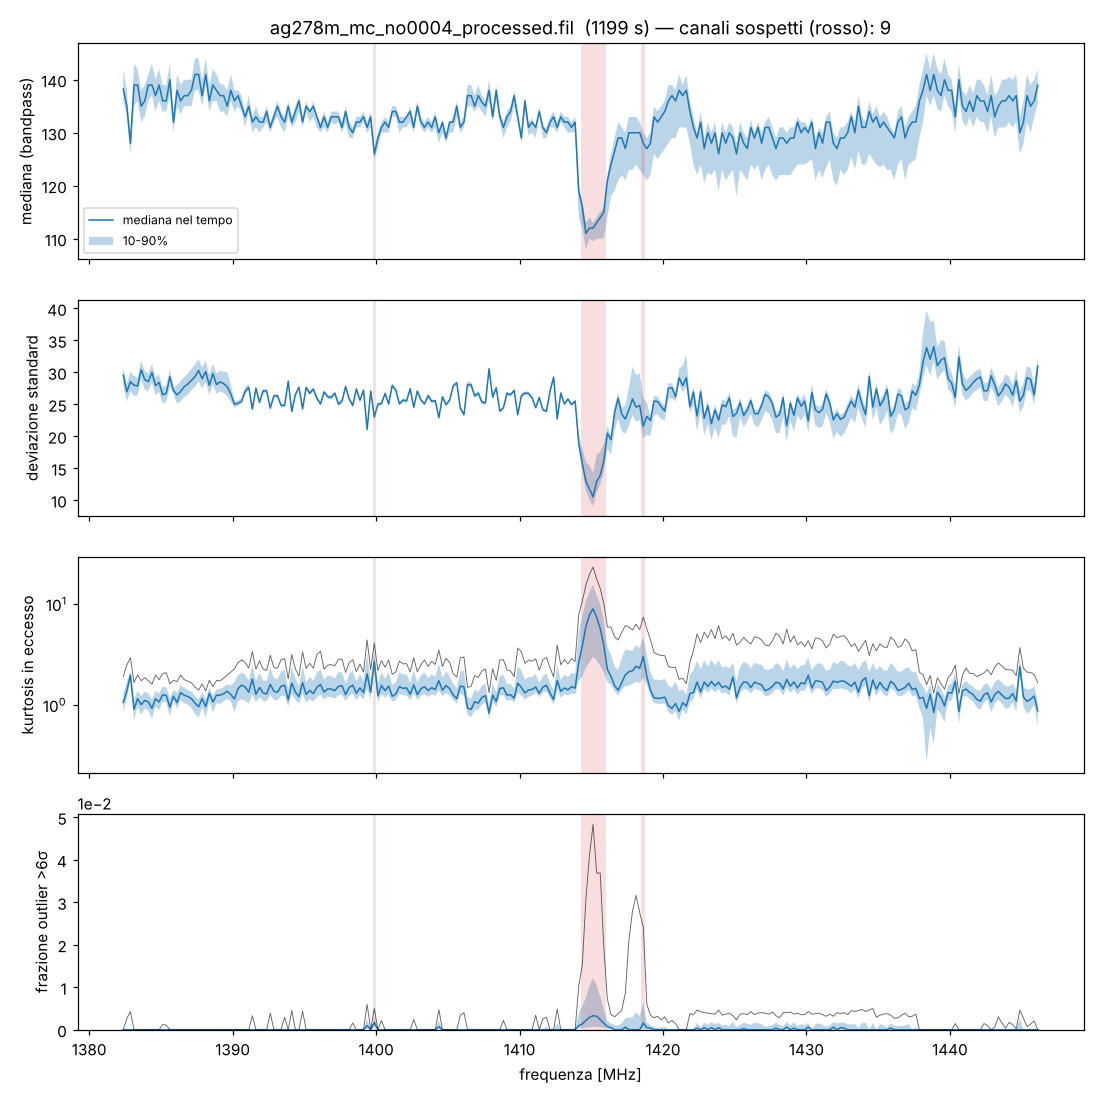
\includegraphics[width=0.86\textwidth]{fig/survey/channels.png}
\caption{Statistiche per canale in funzione della frequenza (blocchi da \SI{4.19}{\second}). Linea blu: mediana nel
tempo; fascia: 10°--90° percentile tra i blocchi; linea nera: massimo tra i blocchi; in rosso i canali segnalati.}
\label{fig:channels}
\end{figure}

\begin{table}[ht]
\centering
\caption{Canali segnalati dal censimento (indici nell'ordine del file; frequenza del centro del canale).}
\label{tab:channels}
\begin{tabular}{rrl}
\toprule
Canale & $\nu$ [MHz] & Motivo \\
\midrule
\tabinput{tab_channels.tex}
\bottomrule
\end{tabular}
\end{table}

Il risultato è in Tabella~\ref{tab:channels} e Figura~\ref{fig:channels}.
\begin{itemize}
  \item \textbf{Canali 121--127} (\SIrange{1414.4}{1415.9}{\mega\hertz}): livello e deviazione standard molto più
    bassi dei canali vicini (livello da \SI{-12}{} a \SI{-16}{\percent}, deviazione standard da \SI{-37}{} a
    \SI{-59}{\percent}), ma kurtosis e frazione di outlier tra le più alte della banda: kurtosis fino a $z\approx30$,
    outlier fino a 0.33\% in mediana e 4.8\% nel blocco peggiore. Lo spettro
    dinamico dei massimi (Fig.~\ref{fig:dynspec}) mostra attività impulsiva continua in questa zona per tutta
    l'osservazione. \ipotesi{La forma del bandpass suggerisce un filtraggio a monte di questa porzione di banda.}
  \item \textbf{Canale 110} (\SI{1418.6}{\mega\hertz}) e la regione fino a \SI{1420}{\mega\hertz}: lampi di outlier
    fino al 2.4\% in alcuni blocchi; segnale intermittente su scale di secondi visibile nello spettro dinamico medio.
  \item \textbf{Canale 185} (\SI{1399.9}{\mega\hertz}): kurtosis moderatamente elevata.
  \item \textbf{La kurtosis in eccesso è positiva in tutti i canali}: mediana 1.41, 10°--90° percentile tra i
    canali 1.08--1.79; per rumore gaussiano sarebbe 0. I dati non sono gaussiani in nessuna parte della banda. Una
    varianza che cambia nel tempo all'interno del blocco produce kurtosis positiva ed è coerente con le variazioni
    di livello descritte nella Sez.~\ref{sec:slow}.
\end{itemize}

\FloatBarrier
\subsection{Struttura in segmenti e variazioni lente a banda larga}
\label{sec:slow}

\begin{figure}[p]
\centering
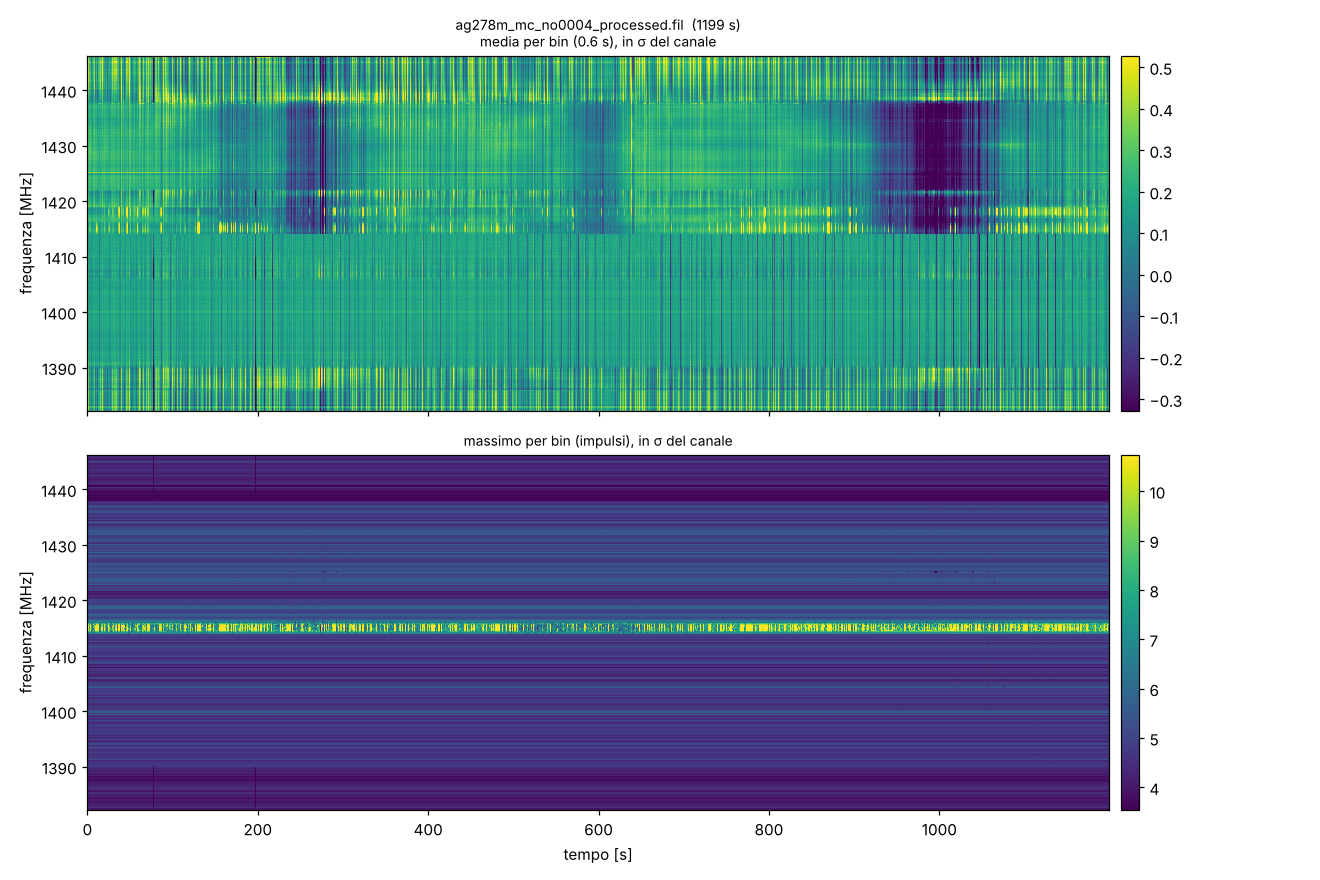
\includegraphics[width=\textwidth]{fig/survey/dynspec.png}
\caption{Spettri dinamici ridotti (bin \SI{0.6}{\second}). In alto la media per bin, sensibile alle variazioni
lente; in basso il massimo per bin, sensibile agli impulsi. Unità: deviazioni standard del singolo campione del
canale.}
\label{fig:dynspec}
\end{figure}

\begin{figure}[ht]
\centering
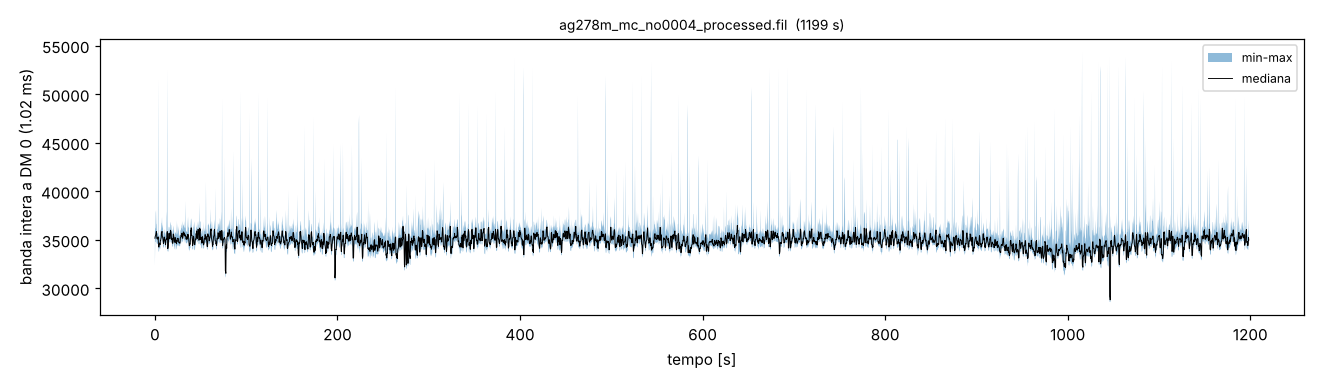
\includegraphics[width=\textwidth]{fig/survey/zerodm.png}
\caption{Serie temporale a DM 0 (somma di tutti i canali, media su \SI{1.024}{\milli\second}), ridotta per la
visualizzazione: fascia = minimo--massimo, linea = mediana.}
\label{fig:zerodm}
\end{figure}

\paragraph{Segmenti della banda.} Lo spettro dinamico medio (Fig.~\ref{fig:dynspec}, in alto) mostra che la banda
si comporta come quattro blocchi:
\begin{itemize}
  \item \SIrange{1414}{1438}{\mega\hertz}: lunghi periodi a livello ridotto (indicativamente
    \SIrange{160}{290}{\second}, \SIrange{570}{620}{\second}, \SIrange{900}{1065}{\second}) con bordi netti in
    frequenza a 1414 e \SI{1438}{\mega\hertz};
  \item sotto \SI{1390}{\mega\hertz} e sopra \SI{1438}{\mega\hertz}: oscillazioni continue su scale di secondi;
  \item \SIrange{1390}{1414}{\mega\hertz}: il segmento più stabile.
\end{itemize}
\ipotesi{La struttura riflette il sistema di acquisizione, per esempio sottobande digitali con guadagno o
riquantizzazione indipendenti. Va verificata con chi conosce il backend di Medicina.}

\paragraph{Rumore comune ai canali.} Nella serie a DM 0 a \SI{1.024}{\milli\second} (64 campioni per bin) la
deviazione standard misurata dalle differenze tra bin adiacenti, $1.4826\,{\rm MAD}(\Delta)/\sqrt2$, vale 170 conteggi.
Se i canali fossero indipendenti ci si aspetterebbero
$(\sum_i\sigma_i^2)^{1/2}/\sqrt{64}=52$ conteggi, usando le deviazioni standard tipiche dei canali. Il rapporto,
\textbf{3.27}, indica una forte componente di rumore comune a tutti i canali già su scale di millisecondi. La stima
attesa è conservativa: le $\sigma_i$ includono anche la variabilità lenta entro i blocchi, quindi il vero eccesso
è almeno questo.

\paragraph{Effetto sulla ricerca a DM bassi.} Alla serie a DM 0 si è sottratta una baseline mobile di
\SI{2}{\second} (mediana) e si sono calcolati boxcar di 1, 8, 32 e \SI{128}{\milli\second}. La
Tabella~\ref{tab:red} confronta due normalizzazioni: con il rumore bianco atteso dalle differenze tra bin
adiacenti, e con la $\sigma$ robusta della serie di boxcar stessa, che è più vicina a ciò che fa Heimdall
normalizzando con il rumore misurato.

\begin{table}[ht]
\centering
\caption{Serie a DM 0 dopo la sottrazione di una baseline mobile di \SI{2}{\second}: frazione del tempo con
$|{\rm S/N}|>8$ secondo due normalizzazioni, e rapporto tra rumore effettivo e rumore bianco.}
\label{tab:red}
\begin{tabular}{rccc}
\toprule
Boxcar & $|{\rm S/N}|>8$, rumore bianco & $|{\rm S/N}|>8$, rumore effettivo & $\sigma_{\rm eff}/\sigma_{\rm bianco}$ \\
\midrule
\SI{1}{\milli\second}   & 1.8\%  & 0.19\% & 2.4 \\
\SI{8}{\milli\second}   & 21.1\% & 0.22\% & 6.0 \\
\SI{32}{\milli\second}  & 48.1\% & 0.07\% & 11.4 \\
\SI{128}{\milli\second} & 69.9\% & 0.05\% & 21.1 \\
\bottomrule
\end{tabular}
\end{table}

\textbf{Correzione rispetto a un'affermazione fatta durante il lavoro.} Nella discussione preliminare (sui primi
\SI{120}{\second}) si era indicato che la serie supera S/N 8 per il 20--70\% del tempo: quel valore usa la
normalizzazione con il rumore bianco. Con la normalizzazione effettiva la frazione scende allo 0.05--0.2\%. Le
variazioni lente quindi \emph{non} sono di per sé una fonte importante di candidati. Il loro effetto principale è
un \textbf{aumento del rumore effettivo sui boxcar larghi}, di un fattore 6--21 tra \SI{8}{\milli\second} e
\SI{128}{\milli\second} rispetto al rumore radiometrico. Questo è una \textbf{perdita di sensibilità} per i burst
larghi. Il calcolo riguarda la serie a DM 0. Per variazioni comuni a tutti i canali più lente dello sweep, la
dedispersione a DM di qualche decina non le attenua, quindi l'effetto è atteso anche nelle serie dedisperse a
DM bassi; questo va verificato.

\FloatBarrier
\subsection{RFI impulsivo a DM 0}
\label{sec:impulsive}

\begin{figure}[ht]
\centering
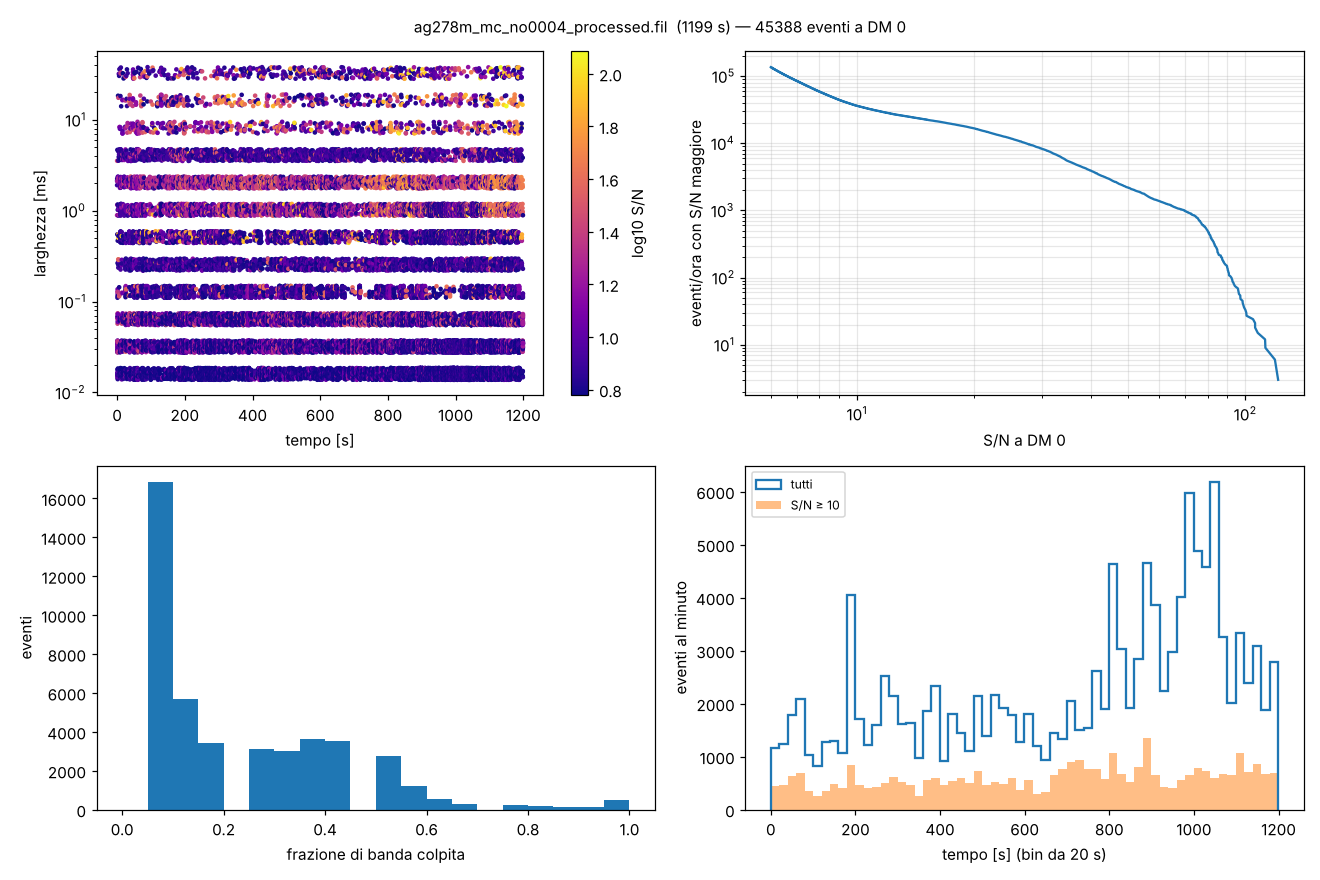
\includegraphics[width=\textwidth]{fig/survey/events.png}
\caption{Eventi impulsivi a DM 0. In alto a sinistra: tempo e larghezza (colore: $\log_{10}$\,S/N; piccolo
spostamento verticale casuale per leggibilità). In alto a destra: frequenza cumulativa degli eventi oltre un dato
S/N. In basso a sinistra: frazione di sottobande colpite. In basso a destra: eventi al minuto (bin \SI{20}{\second}).}
\label{fig:events}
\end{figure}

\begin{table}[ht]
\centering
\caption{Statistiche degli eventi impulsivi a DM 0 sull'intero file.}
\label{tab:events}
\small
\begin{tabular}{lr}
\toprule
Eventi totali (S/N\,$\geq$\,6) & \num{45388} (\SI{37.9}{\per\second}) \\
Frazione del tempo occupata da eventi & 8.9\% \\
Eventi/ora con S/N\,$\geq$\,6, 8, 10, 20 & \num{136278}, \num{58966}, \num{36189}, \num{16730} \\
Eventi/ora con S/N\,$\geq$\,50, 100, 1000 & \num{2189}, 33, 0 \\
Frazione di banda $\leq$25\%, 25--75\%, $>$75\% & \num{29108}, \num{15323}, 957 \\
Larghezza \SIrange{16}{64}{\micro\second} & \num{25016} \\
Larghezza \SIrange{0.128}{1.02}{\milli\second} & \num{14421} \\
Larghezza \SIrange{2.05}{32.8}{\milli\second} & \num{5951} \\
\bottomrule
\end{tabular}
\end{table}

L'RFI impulsivo è presente per tutta l'osservazione (Tab.~\ref{tab:events}, Fig.~\ref{fig:events}).
\begin{itemize}
  \item La maggioranza degli eventi è stretta in frequenza: il 64\% colpisce al più un quarto delle sottobande. Di
    questi, il 66\% ha il massimo nella sottobanda \SIrange{1414}{1418}{\mega\hertz} e il 15\% in
    \SIrange{1390}{1394}{\mega\hertz}.
  \item Il 2\% degli eventi colpisce oltre il 75\% della banda.
  \item La frequenza degli eventi cresce nella seconda metà dell'osservazione (\SIrange{800}{1100}{\second}).
  \item L'S/N massimo a DM 0 è di circa 120: non ci sono impulsi estremamente brillanti.
\end{itemize}

\FloatBarrier
\subsection{Sorgenti periodiche di circa 10 s (radar)}
\label{sec:radar}

\begin{figure}[ht]
\centering
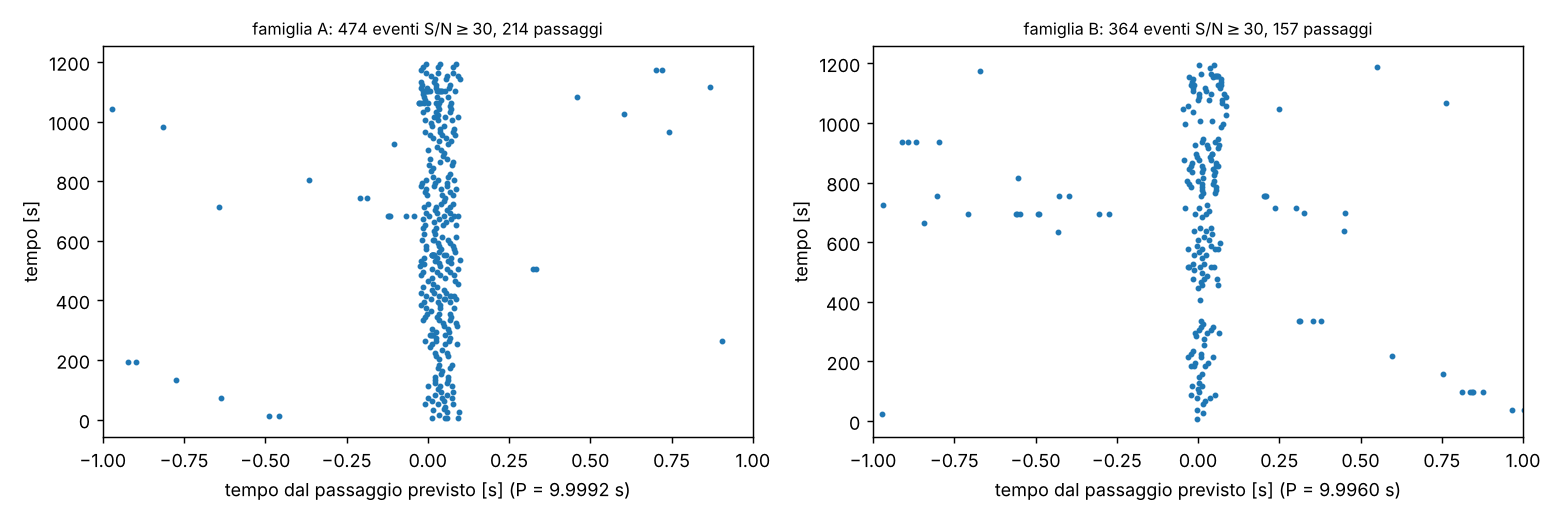
\includegraphics[width=\textwidth]{fig/radar.png}
\caption{Eventi con S/N\,$\geq$\,30 delle due famiglie, in funzione dello scarto dal passaggio previsto con il periodo
stimato (asse x) e del tempo (asse y). La colonna verticale indica una periodicità stabile per tutta l'osservazione.}
\label{fig:radar}
\end{figure}

Gli eventi forti (S/N\,$\geq$\,30) formano due famiglie distinte per la frequenza colpita:
\begin{description}
  \item[Famiglia A] eventi che colpiscono almeno il 90\% della banda;
  \item[Famiglia B] eventi limitati alla metà inferiore della banda (\SIrange{1382}{1414}{\mega\hertz}): almeno 7
    delle 8 sottobande basse colpite e al più 2 delle 8 alte.
\end{description}
Gli eventi entro \SI{1}{\second} l'uno dall'altro sono raggruppati in ``passaggi''. Il periodo è stimato con una
scansione di Rayleigh sui primi impulsi dei passaggi (\SIrange{5}{15}{\second}), seguita da un fit lineare
$t=t_0+nP$ dei passaggi coerenti (scarto $<\SI{0.3}{\second}$).

\begin{table}[ht]
\centering
\caption{Parametri delle due sorgenti periodiche. L'errore su $P$ è quello formale del fit.}
\label{tab:radar}
\begin{tabular}{lcc}
\toprule
 & Famiglia A (banda intera) & Famiglia B (metà bassa) \\
\midrule
Eventi con S/N\,$\geq$\,30 & 474 & 364 \\
Passaggi / passaggi coerenti & 214 / 112 & 157 / 84 \\
Cicli coperti dall'osservazione & 120 & 120 \\
Periodo $P$ [s] & $9.99924\pm0.00016$ & $9.99598\pm0.00008$ \\
Fase $t_0$ [s] & 3.636 & 6.158 \\
Scarto quadratico medio dei passaggi [ms] & 58 & 26 \\
Impulsi per passaggio (mediana) & 2 & 2 \\
Spaziatura tra impulsi (mediana) & \SI{38.4}{\milli\second} & \SI{38.5}{\milli\second} \\
\bottomrule
\end{tabular}
\end{table}

Interpretazione (Tab.~\ref{tab:radar}, Fig.~\ref{fig:radar}):
\begin{itemize}
  \item entrambe le famiglie sono presenti per tutti i \SI{1200}{\second}, nel 93\% (A) e nel 70\% (B) dei cicli;
  \item la differenza tra i periodi, \SI{3.3}{\milli\second}, è formalmente molto significativa. Però gli impulsi
    sono spaziati di \SI{38}{\milli\second} entro un passaggio, e scegliere il ``primo impulso'' può introdurre
    errori sistematici non inclusi nell'errore formale. Il risultato è indicativo di due sorgenti distinte, ma non
    conclusivo;
  \item circa metà dei passaggi forti della famiglia A non è coerente con il periodo: ci sono altre sorgenti
    impulsive a banda larga non periodiche;
  \item \ipotesi{Rotazioni di circa \SI{10}{\second} e la banda \SIrange{1215}{1400}{\mega\hertz} sono tipiche dei
    radar di sorveglianza aerea a lungo raggio. La famiglia B, confinata sotto \SI{1414}{\mega\hertz}, è compatibile
    con un radar che opera appena sotto la banda osservata.}
\end{itemize}
Nota sullo strumento: la ricerca automatica di periodicità del censimento \emph{non} riporta direttamente i
\SI{10}{\second}, perché le due famiglie sono diluite tra gli altri eventi; questi risultati derivano dall'analisi
dedicata descritta sopra, che andrà integrata nello strumento.

\FloatBarrier
\subsection{Altre periodicità}
\label{sec:period}

\begin{table}[ht]
\centering
\caption{Periodicità principali trovate dal censimento (estratto di \file{periodicity.csv}). ``Armonica'' è la
frequenza del picco più forte nello spettro sommato; $\sigma$ è la significatività formale (assume rumore bianco
gaussiano e va letta solo come ordine di grandezza); $Z$ è il test di Rayleigh per i treni di eventi.}
\label{tab:period}
\small
\begin{tabular}{lrrrrr}
\toprule
Serie & $f$ [Hz] & $P$ [s] & Armonica [Hz] & $\sigma$ & $Z$ \\
\midrule
\tabinput{tab_periodicity.tex}
\bottomrule
\end{tabular}
\end{table}

Dalla Tabella~\ref{tab:period}:
\begin{itemize}
  \item \textbf{\SI{50}{\hertz}} ($P=\SI{0.0200000}{\second}$) è la periodicità dominante sia nella serie a DM 0 sia nei
    treni di eventi (Rayleigh $Z\approx\numrange{360}{400}$). \ipotesi{Interferenza dalla rete elettrica.}
  \item Due periodicità sono \textbf{esatte} entro $10^{-6}$ in frazione: \SI{0.625000}{\second} (\SI{1.6}{\hertz}) e
    \SI{0.400000}{\second} (\SI{2.5}{\hertz}), con armoniche forti a 40 e \SI{75}{\hertz}.
    \ipotesi{Periodi così stabili indicano sorgenti artificiali agganciate a un riferimento di tempo, oppure un
    effetto del sistema di acquisizione (per esempio la struttura dei pacchetti).}
  \item Ci sono altre periodicità di decine di Hz (30, 33.3, 46.875, \SI{66.7}{\hertz} e altre) di origine non
    determinata.
\end{itemize}

\FloatBarrier
\subsection{Candidati di Heimdall e classificazione FETCH}
\label{sec:cands}

\begin{figure}[ht]
\centering
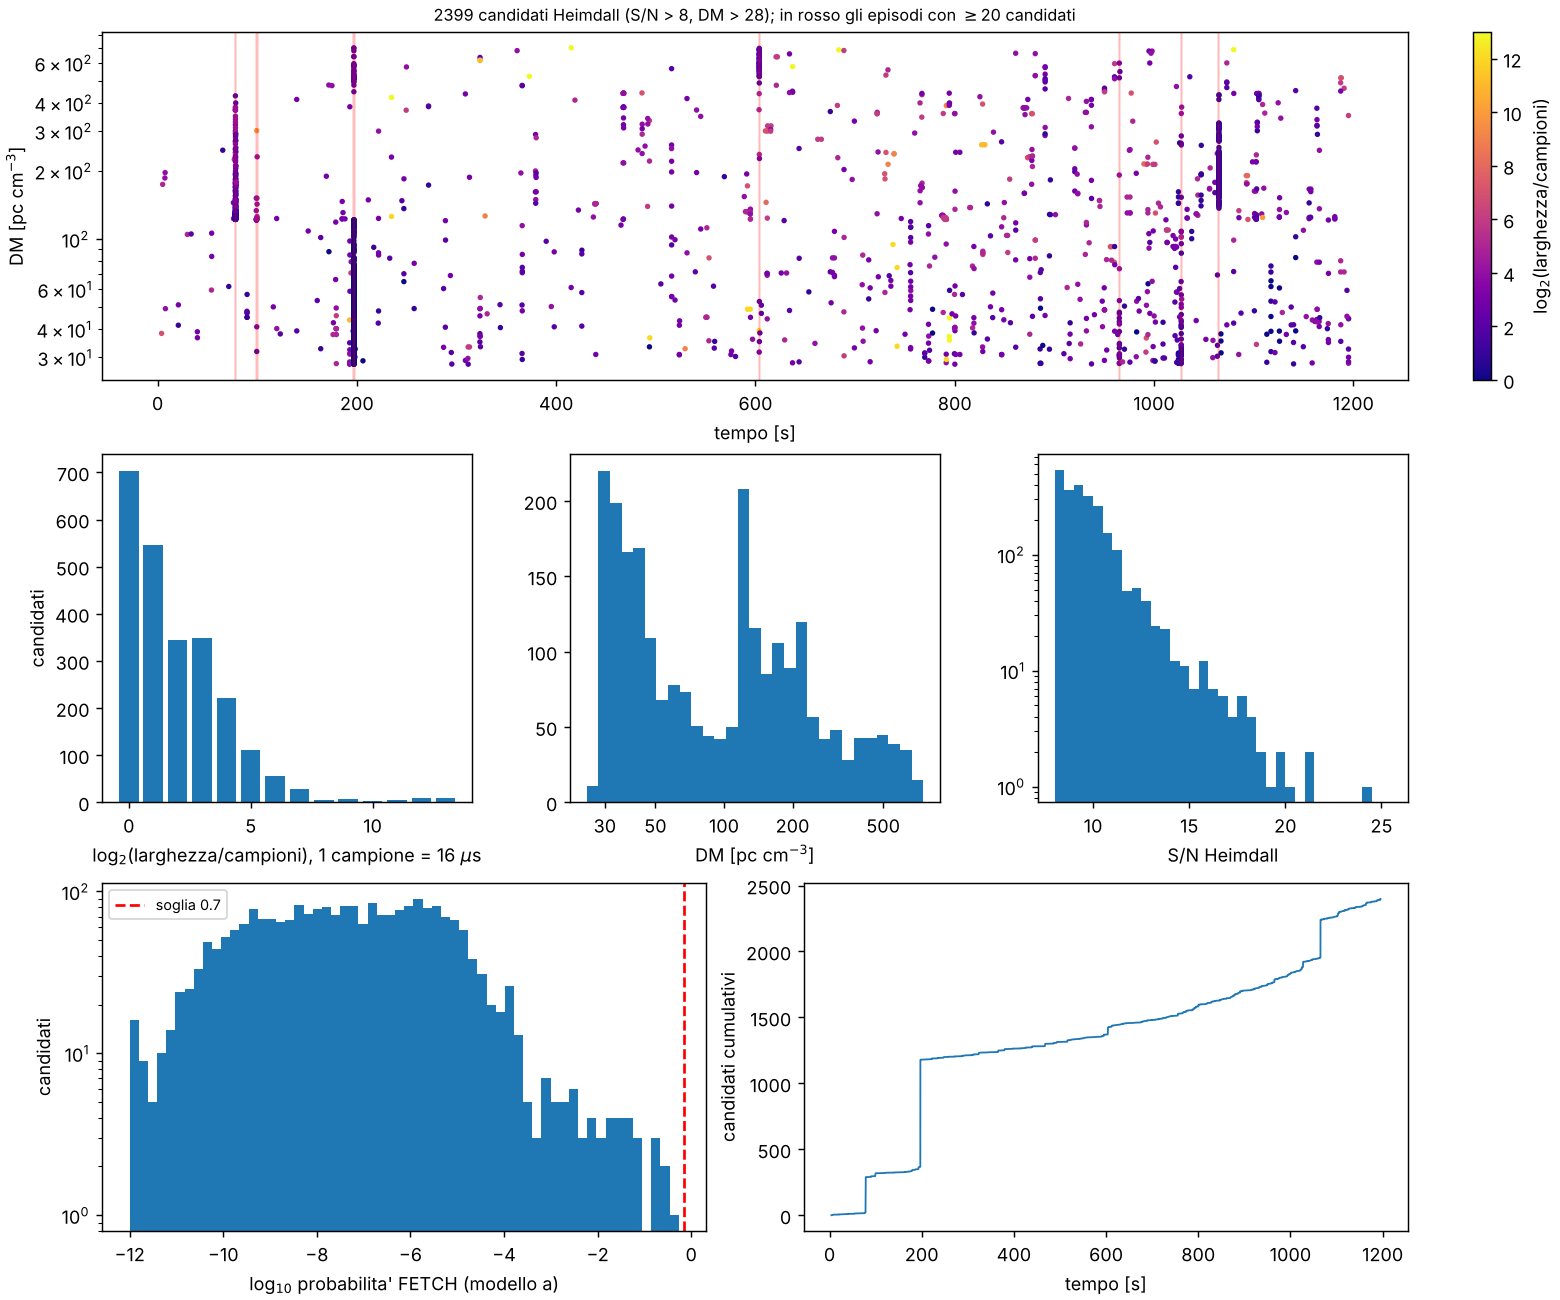
\includegraphics[width=\textwidth]{fig/candidates.png}
\caption{Candidati di Heimdall dopo la selezione S/N\,$>$\,8, DM\,$>$\,28. In alto: DM e tempo (colore: $\log_2$ della
larghezza in campioni); in rosso gli episodi con almeno 20 candidati. Al centro: distribuzioni di larghezza, DM e
S/N. In basso: distribuzione della probabilità FETCH e numero cumulativo di candidati.}
\label{fig:cands}
\end{figure}

\begin{itemize}
  \item \textbf{2399 candidati} in \SI{1199}{\second} (\SI{3.99}{}--\SI{1195.17}{\second}), con S/N tra 8.0 e 24.4
    (mediana 9.4) e DM con percentili 5/25/50/75/95 pari a 30, 40, 93, 184 e 497.
  \item \textbf{Sono quasi tutti stretti}: l'81\% ha larghezza tra 1 e 8 campioni
    (\SIrange{16}{128}{\micro\second}); solo 40 sono larghi almeno \SI{4.1}{\milli\second} ($k\geq8$).
  \item \textbf{FETCH} ha classificato tutti i 2399 candidati: probabilità mediana $4.5\times10^{-8}$, 99° percentile
    0.007, massimo 0.54. Un solo candidato supera 0.5 e nessuno raggiunge la soglia di 0.7, quindi
    \file{Best_candidates.csv} è vuoto.
  \item I cinque candidati più probabili sono larghi 33--\SI{66}{\milli\second}: tre a DM 260.9 (a 827.0, 829.0 e
    \SI{830.2}{\second}; probabilità 0.19, 0.54, 0.20), uno a \SI{192.7}{\second} (DM 43.9, 0.31) e uno a
    \SI{738.0}{\second} (DM 94.6, 0.27). La loro natura non è stata ancora esaminata.
\end{itemize}
\textbf{Correzione:} in una fase preliminare si era indicato che 58 candidati non avessero un file \file{.h5}.
Era un errore dell'abbinamento: la coppia (tempo, DM) non è univoca. Con l'abbinamento su (tempo, DM, S/N) tutti
i candidati risultano classificati.

\FloatBarrier
\subsection{Episodi di candidati}
\label{sec:episodes}

Raggruppando i candidati separati da meno di \SI{0.5}{\second}, \textbf{1509 candidati (63\%) cadono in 7 episodi
di durata inferiore al secondo} (Tab.~\ref{tab:episodes}). Gli altri 890 (44.5 al minuto, larghezza mediana
$2^3$ campioni, DM mediana 105) formano un fondo diffuso.

\begin{table}[ht]
\centering
\caption{Episodi con almeno 20 candidati. $k$: $\log_2$ della larghezza in campioni (mediana). Livello ai bordi e al
centro: variazione minima/massima, in un intorno di $\pm\SI{1.5}{\second}$, del livello medio delle 4 sottobande ai
bordi (1382--1390 e \SIrange{1438}{1446}{\mega\hertz}) e delle 12 centrali, rispetto ai \SIrange{2}{6}{\second}
precedenti. Rumore 1416: massimo, nello stesso intorno, della deviazione standard della sottobanda
\SIrange{1414}{1418}{\mega\hertz} (bin \SI{0.25}{\second}) rispetto al suo valore tipico. Salto: massima variazione
del livello ai bordi tra bin consecutivi da \SI{0.25}{\second}. Tra parentesi la probabilità che una finestra
casuale della stessa durata mostri un valore almeno pari.}
\label{tab:episodes}
\footnotesize
\setlength{\tabcolsep}{4pt}
\begin{tabular}{lrrrrrrrrr}
\toprule
Intervallo [s] & $N$ & DM & $k$ & S/N$_{\max}$ & $P^{\rm FETCH}_{\max}$ & Bordi [\%] & Centro [\%] & Rumore 1416 & Salto [\%] \\
\midrule
\tabinput{tab_episodes.tex}
\bottomrule
\end{tabular}
\end{table}

\begin{figure}[ht]
\centering
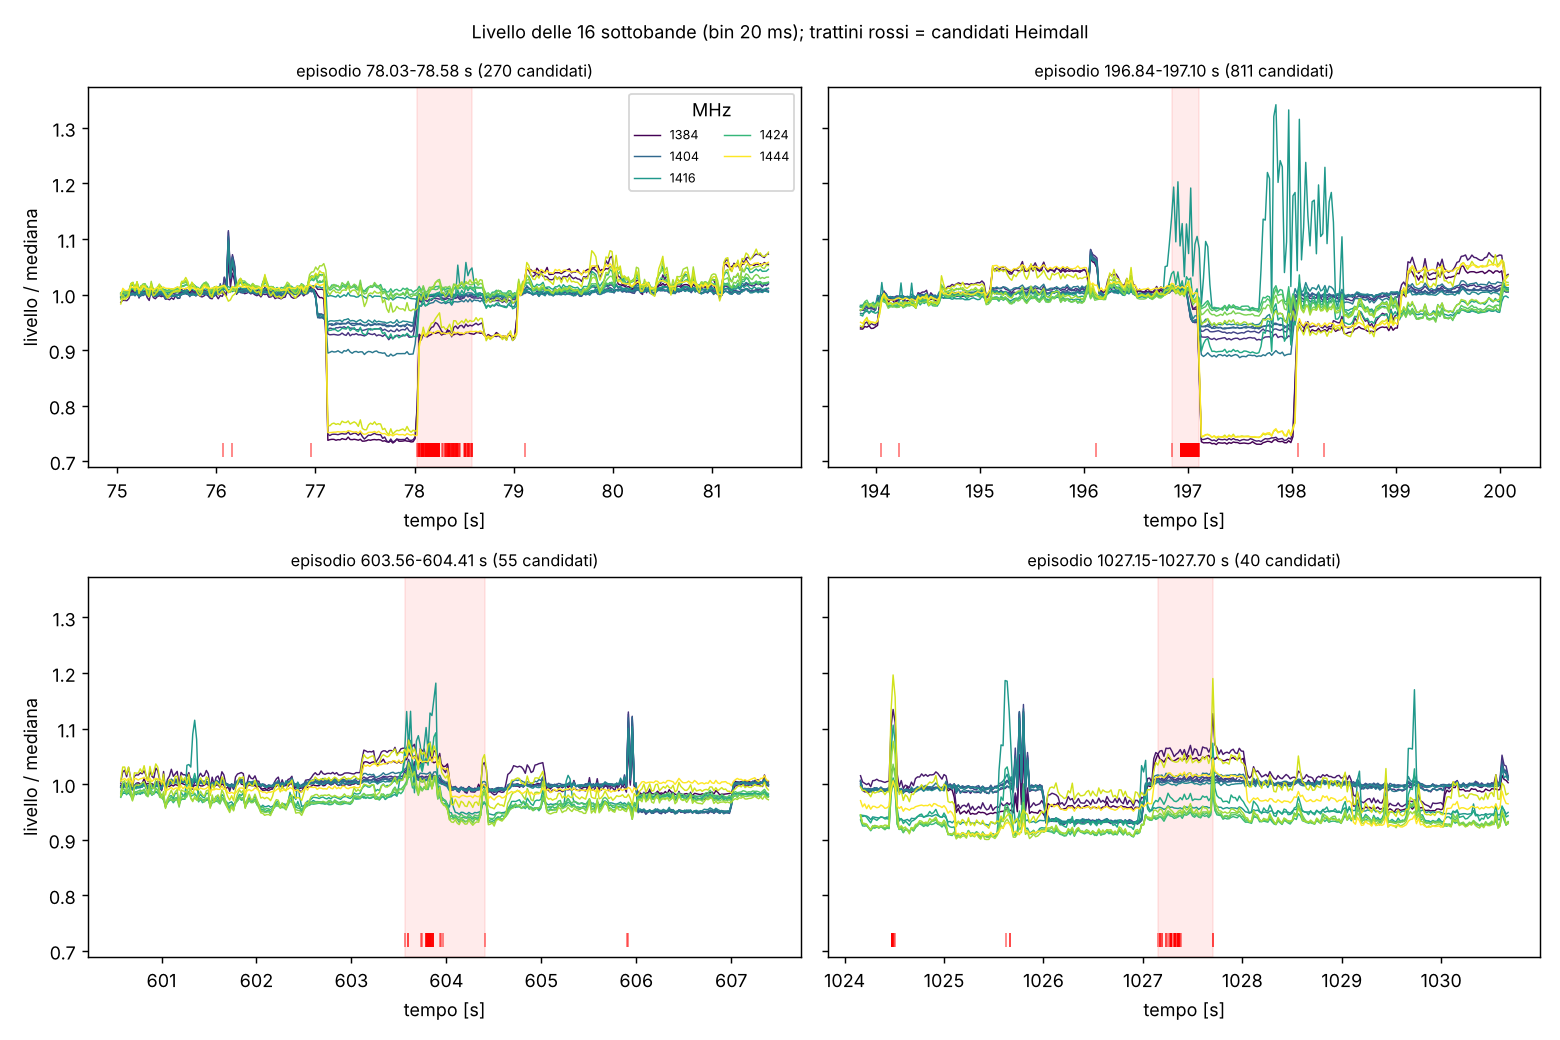
\includegraphics[width=\textwidth]{fig/episodes_subbands.png}
\caption{Livello delle 16 sottobande (media su \SI{20}{\milli\second}, normalizzata alla mediana) attorno a quattro
episodi. I trattini rossi sono i tempi dei candidati di Heimdall; la fascia rosa è l'intervallo dell'episodio.}
\label{fig:episodes}
\end{figure}

\paragraph{Episodio a \SI{78}{\second} (270 candidati).} A \SI{77.11}{\second} il livello di tutta la banda scende
bruscamente: circa \SI{-26}{\percent} nelle sottobande ai bordi e da \SI{-5}{} a \SI{-10}{\percent} al centro
(Fig.~\ref{fig:episodes}). Il ritorno avviene in due gradini, a \SI{78.03}{\second} e a \SI{79.05}{\second}. I
candidati iniziano a \SI{78.026}{\second}, in corrispondenza del primo gradino, e terminano a \SI{78.58}{\second}.
Il salto è significativo ($p<0.01$); il rumore a 1416 MHz non lo è ($p=0.85$). I livelli discreti (circa 0.74 e
0.93 della mediana ai bordi) fanno pensare a passi discreti di guadagno o di attenuazione. \ipotesi{Un controllo
automatico del guadagno a gradini.}

\paragraph{Episodio a \SI{197}{\second} (811 candidati).} A \SI{196.85}{\second} il rumore della sottobanda
\SIrange{1414}{1418}{\mega\hertz} aumenta fino a 25 volte il valore tipico ($p<0.01$). I candidati, larghi un solo
campione e distribuiti su tutti i DM tra 28 e 699, coincidono con questo intervallo (196.84--\SI{197.10}{\second}).
A \SI{197.12}{\second} segue un calo di livello di tutta la banda con la stessa forma dell'episodio a
\SI{78}{\second} (bordi a 0.74), che rientra a \SI{198.05}{\second}. \ipotesi{Il calo di guadagno potrebbe essere
la reazione di un controllo automatico al lampo di RFI.} Va notato che un secondo intervallo di forte rumore a
\SI{1416}{\mega\hertz}, tra 197.5 e \SI{198.0}{\second} durante il calo di livello, produce solo un paio di
candidati: il motivo non è chiarito.

\paragraph{Altri episodi.} Per gli episodi a 99, 604, 965, 1027 e \SI{1065}{\second} i valori massimi di rumore e
di salto nell'intorno non sono significativi singolarmente ($p$ tra 0.12 e 0.85): la loro origine
\textbf{non è stabilita} da questa analisi. Gli episodi a 604 e \SI{1027}{\second} mostrano comunque, nella
Fig.~\ref{fig:episodes}, variazioni di livello di qualche percento e picchi nelle sottobande centrali durante
l'intervallo.

\FloatBarrier
\subsection{Associazione statistica tra candidati e disturbi}
\label{sec:correlation}

\begin{figure}[ht]
\centering
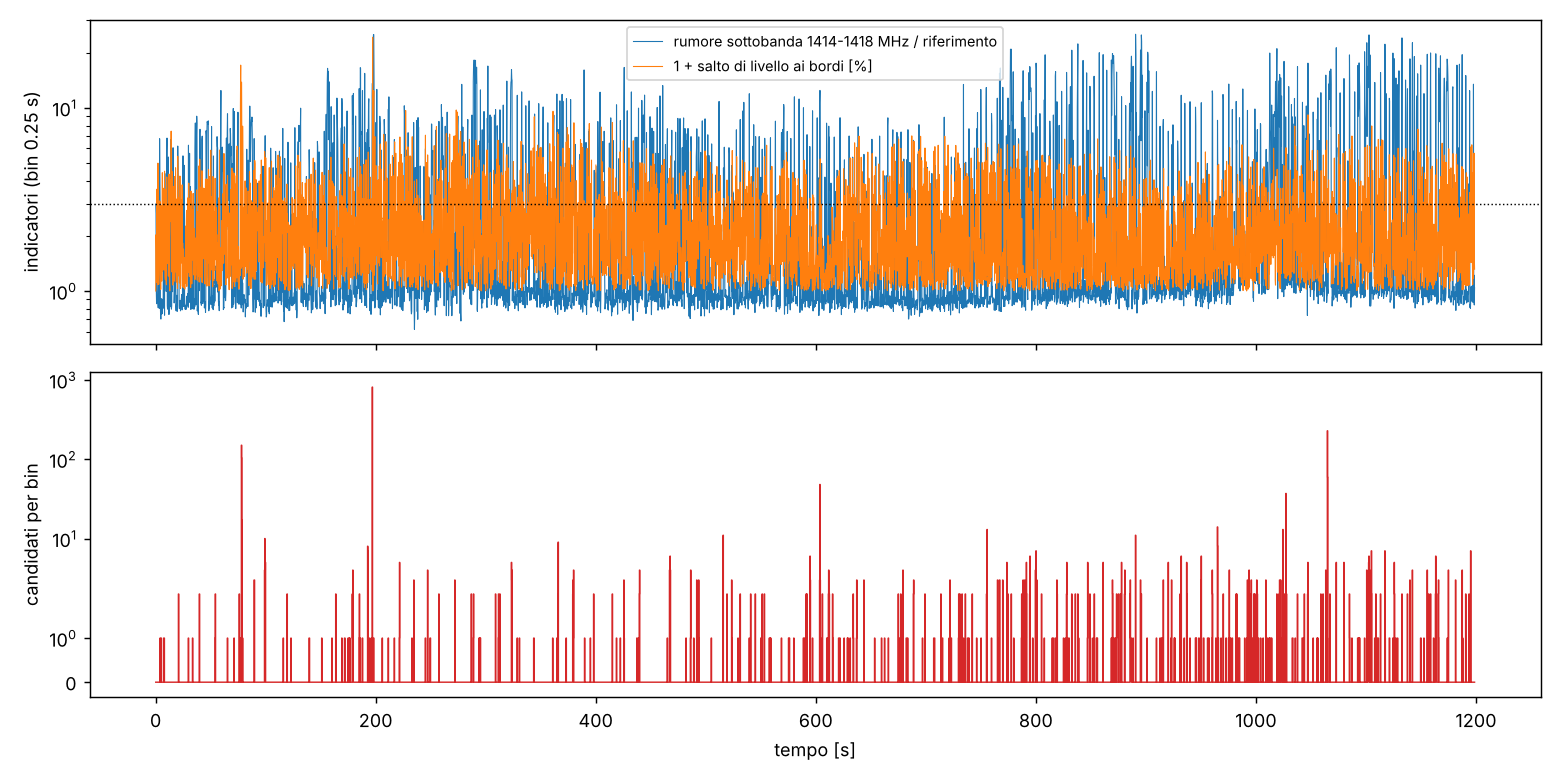
\includegraphics[width=\textwidth]{fig/correlation.png}
\caption{In alto: indicatori per intervalli da \SI{0.25}{\second}, cioè il rumore della sottobanda
\SIrange{1414}{1418}{\mega\hertz} rispetto al valore tipico e $1+{}$salto di livello ai bordi in percentuale (la
linea tratteggiata, a 3, corrisponde alle soglie della riga centrale della Tab.~\ref{tab:corr}). In basso:
candidati di Heimdall per intervallo.}
\label{fig:corr}
\end{figure}

L'osservazione è stata divisa in 4798 intervalli da \SI{0.2499}{\second} (244 bin della serie a DM 0) e ogni intervallo è stato classificato con due
indicatori:
\begin{description}
  \item[A] rumore della sottobanda \SIrange{1414}{1418}{\mega\hertz} superiore a $X$ volte il valore tipico;
  \item[B] salto del livello medio delle sottobande ai bordi, rispetto all'intervallo precedente, superiore a $Y$.
\end{description}

\begin{table}[ht]
\centering
\caption{Frazione del tempo e dei candidati negli intervalli da \SI{0.25}{\second} classificati con gli indicatori A e
B, per tre coppie di soglie. ``Densità'' è il numero medio di candidati per intervallo diviso per la media su tutto il
file.}
\label{tab:corr}
\small
\begin{tabular}{rrlrrrr}
\toprule
$X$ & $Y$ & Condizione & Tempo & Candidati & Frazione & Densità \\
\midrule
\tabinput{tab_correlation.tex}
\bottomrule
\end{tabular}
\end{table}

Con le soglie intermedie ($X=3$, $Y=2\%$), gli intervalli con A oppure B coprono il \textbf{39.4\% del tempo e
contengono l'87.4\% dei candidati}. Il restante 60.6\% del tempo contiene il 12.6\% dei candidati, con densità 0.21
volte la media (Tab.~\ref{tab:corr}). L'associazione resta per tutte e tre le coppie di soglie.

Siccome i due episodi a 78 e \SI{197}{\second} pesano molto sul totale (1081 candidati), l'analisi è stata ripetuta
escludendoli. Con $X=3$, $Y=2\%$: A oppure B copre il 39.4\% del tempo e contiene il \textbf{77.1\%} dei candidati
rimanenti (densità 1.96); gli intervalli senza A né B contengono il 22.9\% (densità 0.38).

\paragraph{Cautele.}
\begin{itemize}
  \item I candidati sono fortemente raggruppati nel tempo, quindi non si può attribuire un valore $p$ semplice a
    questi rapporti (i conteggi non sono poissoniani).
  \item Un'associazione non implica un rapporto di causa: A e B potrebbero essere manifestazioni di un fattore
    comune, per esempio un RFI forte che produce sia il rumore sia la reazione del guadagno.
  \item Le soglie sono state scelte dopo aver visto i dati; la stabilità rispetto alle tre coppie di soglie riduce,
    ma non elimina, questo effetto.
  \item Il riferimento temporale di \texttt{stime} di Heimdall (frequenza di riferimento) non è stato verificato;
    con bin da \SI{0.25}{\second} e sweep fino a \SI{132}{\milli\second} l'effetto sulla classificazione è al più
    marginale.
\end{itemize}

% =====================================================================================
\FloatBarrier
\section{Discussione dell'analisi iniziale}
\label{sec:discussion}

\paragraph{Cosa genera i candidati in questa osservazione.} I dati indicano che la maggior parte dei candidati di
Heimdall \emph{non} è la versione dedispersa di impulsi forti a DM 0: i candidati sono stretti
(\SIrange{16}{128}{\micro\second}), mentre un impulso non disperso a DM\,$\geq$\,28 verrebbe allargato su
$\geq\SI{5}{\milli\second}$. Inoltre nei primi \SI{120}{\second} l'associazione con gli impulsi radar è al livello
casuale (21\% contro 22\%). L'ipotesi preliminare in questo senso va quindi scartata come spiegazione principale.

I candidati si concentrano invece in brevi intervalli in cui cambiano bruscamente il livello o la varianza dei dati:
salti di guadagno a banda larga, più forti ai bordi, e lampi di rumore nella zona
\SIrange{1414}{1418}{\mega\hertz}.
\ipotesi{Il meccanismo proposto è che Heimdall normalizzi le serie dedisperse con una stima del rumore che non segue
cambiamenti rapidi della varianza. Per qualche centinaio di millisecondi le normali fluttuazioni producono S/N\,$>$\,8
a molti DM e con larghezze piccole.} L'ipotesi è coerente con l'episodio a \SI{197}{\second} (811 candidati larghi
un campione a tutti i DM), ma non è verificata direttamente sul codice di Heimdall.

\paragraph{Implicazioni per la pulizia.} In ordine di impatto atteso:
\begin{enumerate}
  \item \textbf{Mascherare i canali 121--127}, oltre a 110 e 185, che concentrano l'attività impulsiva della zona
    \SIrange{1414}{1418}{\mega\hertz}.
  \item \textbf{Normalizzare ogni canale con media e deviazione standard mobili} su scale di
    \SIrange{0.1}{0.5}{\second}, con stime robuste agli impulsi. I salti di guadagno sono più forti ai bordi, quindi
    vanno trattati come moltiplicativi e canale per canale.
  \item \textbf{Riconoscere e sostituire i tratti con varianza anomala.}
  \item \textbf{Rimuovere gli impulsi forti a DM 0} (radar), con un veto sulla dispersione che dipenda dalla larghezza
    (Sez.~\ref{sec:data}). In questa osservazione sembra meno rilevante per il numero di candidati.
\end{enumerate}
Inoltre la Tabella~\ref{tab:red} indica che il rumore effettivo sui boxcar larghi è molto superiore a quello
radiometrico. Una normalizzazione efficace delle variazioni lente potrebbe quindi migliorare anche la
\emph{sensibilità} ai burst larghi, oltre a ridurre i falsi positivi. Va verificato con le iniezioni.

\paragraph{Limiti di questa analisi.}
\begin{itemize}
  \item È stata analizzata una sola osservazione.
  \item La causa di 5 episodi su 7 non è stabilita.
  \item L'analisi dei candidati parte dall'output già filtrato (S/N\,$>$\,8, DM\,$>$\,28) e non dai file
    \file{.cand} completi di Heimdall.
  \item La calibrazione dell'S/N dell'iniettore su Heimdall non è ancora stata eseguita.
  \item Nessun burst sintetico è ancora stato iniettato in questi dati, quindi la sensibilità della pipeline attuale
    non è stata misurata.
\end{itemize}
Le sezioni seguenti descrivono come queste indicazioni sono state tradotte nella pipeline di pulizia. Gli ultimi due
limiti sono stati affrontati: la calibrazione dell'S/N su Heimdall e la sensibilità sono misurate nel pilota della
campagna di completezza (Sez.~\ref{sec:completeness}). L'ipotesi sul meccanismo degli episodi è coerente con il fatto
che la normalizzazione dello step 1, che segue i salti di guadagno, li elimina tutti (Sez.~\ref{sec:step1}).

% =====================================================================================
% Parte II: la pipeline di pulizia (incluso da report.tex)
% =====================================================================================
\FloatBarrier
\section{La pipeline di pulizia}
\label{sec:cleanpipe}

Sulla base dell'analisi iniziale (Sez.~\ref{sec:results} e~\ref{sec:discussion}) è stata costruita una pipeline
in quattro passi, da eseguire in quest'ordine prima della ricerca con \file{FRB_HF_Finder.py}:
\begin{center}
\begin{tabular}{llp{9.2cm}}
\toprule
Step & Strumento & Cosa rimuove \\
\midrule
1 & \file{tools/rfi_clean.py} & canali cattivi, salti di guadagno, variazioni lente del livello e del rumore, celle
  tempo--frequenza con varianza anomala \\
2 & \file{tools/rfi_periodic.py} & RFI periodico (rete elettrica a \SI{50}{\hertz} e armoniche, e qualsiasi altra
  famiglia di righe) \\
3 & \file{tools/rfi_impulses.py} & impulsi a DM 0 a banda intera o parziale (radar), con veto di dispersione \\
4 & \file{tools/rfi_commonmode.py} & rumore di modo comune, cioè la componente correlata tra tutti i canali \\
\bottomrule
\end{tabular}
\end{center}

\paragraph{Principi comuni.}
\begin{itemize}
  \item \textbf{Generalità.} Nessuno step contiene valori specifici di questa osservazione. Le soglie sono espresse in
    sigma, frazioni o secondi; le grandezze strumentali (campionamento, frequenze, numero di canali, numero di bit,
    ritardi di dispersione) sono lette dall'header o stimate dai dati. I valori di default sono stati scelti e
    validati su dati sintetici costruiti con lo stesso setup di Medicina (banda L, \SI{64}{\mega\hertz}, 256 canali,
    \SIrange{16}{64}{\micro\second}).
  \item \textbf{Protezione dei segnali dispersi.} Ogni step che sostituisce o sottrae dati ha un meccanismo che non
    tocca, o tocca in misura nota, un segnale disperso: veto di dispersione negli step 1 e 3, test di dispersione sulle
    famiglie periodiche nello step 2, perdita limitata alla frazione larghezza/sweep nello step 4.
  \item \textbf{Formato invariato.} L'output di ogni step è un filterbank con lo stesso header e lo stesso numero di
    bit; con dati interi l'arrotondamento è stocastico (\emph{dithering}), così le correzioni inferiori a un
    conteggio sono conservate in media. Ogni step scrive un riassunto (\file{.json}) e i dati diagnostici
    (\file{.npz}, \file{.csv}).
  \item \textbf{Memoria e tempi.} Tutti gli step leggono il file a blocchi: la memoria non dipende dalla dimensione
    del file. Sul file intero (\SI{19}{\giga\byte}) ogni step richiede da circa \SI{20}{} a \SI{35}{\minute}.
  \item \textbf{Validazione.} Ogni step ha test automatici su dati sintetici (\file{tests/}, 47 test), che verificano sia
    la rimozione degli RFI sia la conservazione dell'S/N di FRB iniettati.
\end{itemize}

L'ordine non è arbitrario. Lo step 1 rende i canali confrontabili (stessa scala) e maschera quelli inutilizzabili:
tutti gli step successivi ne hanno bisogno. Gli step 2 e 3 lavorano sulle serie a DM 0 (banda intera e sottobande),
che lo step 4 azzera per costruzione, e lo step 3 toglie gli impulsi a banda parziale che una sottrazione del modo
comune trasformerebbe in impronte negative negli altri canali. Lo step 4 è quindi l'ultimo.

% -------------------------------------------------------------------------------------
\FloatBarrier
\section{Step 1: maschera, normalizzazione e celle anomale}
\label{sec:step1}

\paragraph{Metodo.} Due passaggi sul file.
\begin{enumerate}
  \item \textbf{Statistiche.} Per ogni canale e finestra di \SI{0.2}{\second} si stimano livello e rumore con media e
    deviazione standard troncate a $3\sigma$ robuste, su un sottocampione. Le serie di livello e rumore sono filtrate con
    una mediana mobile su 5 finestre, che conserva i gradini ma ignora i disturbi più brevi. Dagli stessi blocchi si
    ricava la \textbf{maschera automatica}: un canale è mascherato se, nei blocchi da \SI{4}{\second}, il suo rumore, la
    curtosi o la frazione di campioni anomali si discostano dagli altri canali con $z$ robusto $>5$.
  \item \textbf{Salti di guadagno.} Prima delle statistiche si cercano i salti di livello con un filtro a gradino
    (due lati da \SI{20}{\milli\second}, risoluzione \SI{0.5}{\milli\second}) su 16 sottobande, con soglia $6\sigma$ e un
    test di persistenza: il nuovo livello deve durare almeno \SI{0.2}{\second}, cosa che un burst non fa. Le finestre
    delle statistiche non attraversano mai un salto, e la normalizzazione è interpolata solo all'interno di ciascun
    segmento.
  \item \textbf{Pulizia.} Ogni campione è normalizzato, $z=(x-\text{livello}(t))/\text{rumore}(t)$, con livello e
    rumore interpolati a \SI{1}{\milli\second}. I dati sono divisi in celle di \SI{8}{\milli\second} per canale; si
    sostituiscono con rumore gaussiano le celle con varianza anomala oltre $6\sigma$ robuste. La varianza è stimata
    dalle \emph{differenze} tra campioni consecutivi, quindi un segnale liscio come un FRB largo più di pochi campioni
    quasi non la modifica. Se in un intervallo sono anomali più della metà dei canali si sostituisce l'intero
    intervallo, ma solo dopo un \textbf{veto di dispersione}: si protegge l'intervallo se esiste una traccia con
    DM\,$\geq$\,15 il cui S/N supera di 1.2 volte quello a DM 0 ed è almeno 7.
  \item \textbf{Uscita.} $y=128+8z$ per dati a 8 bit (dinamica $\pm16\sigma$); i canali mascherati sono costanti.
\end{enumerate}

\paragraph{Risultati su \file{ag278m_mc_no0004}.}
\begin{itemize}
  \item Maschera: canali 121--127 (\SIrange{1414.4}{1415.9}{\mega\hertz}) e 185 (\SI{1399.9}{\mega\hertz}), in accordo
    con l'analisi iniziale (Sez.~\ref{sec:results}).
  \item Trovati 1366 salti di guadagno reali, distanziati in media di circa \SI{1}{\second} e più forti ai bordi della
    banda, compatibili con un controllo automatico del guadagno. \ipotesi{L'attribuzione al controllo automatico del
    guadagno del backend non è verificata con chi conosce lo strumento.}
  \item Ricerca dopo il solo step 1 (prima versione): da 2399 a 816 candidati; i 7 episodi dell'analisi iniziale
    (Sez.~\ref{sec:episodes}) scompaiono tutti; la frazione di candidati stretti ($\leq2^3$ campioni) scende dall'81\%
    al 16\%. Due candidati superano la soglia di FETCH: all'ispezione sono RFI.
\end{itemize}

\paragraph{Correzioni durante lo sviluppo.} La prima versione non gestiva i salti di guadagno (da cui la ricerca dei
salti); distruggeva i burst più brillanti (da cui la varianza dalle differenze, il test di persistenza, l'uscita a
$\pm16\sigma$ e il veto di dispersione); la maschera era poco sensibile sui dati reali (da cui le statistiche per
blocchi come nel censimento); il veto era lento (da cui una griglia di DM più rada con confronto a basso DM).

% -------------------------------------------------------------------------------------
\FloatBarrier
\section{Step 2: RFI periodico}
\label{sec:step2}

\paragraph{Metodo.} Completamente automatico: non richiede di indicare le frequenze.
\begin{enumerate}
  \item \textbf{Spettro.} Spettro di potenza (Welch, finestra di Hann) della serie a DM 0 a banda intera, alla
    risoluzione nativa fino alla frequenza di Nyquist, quindi senza aliasing. Le righe sono i massimi locali del
    rapporto spettro/continuo (mediana mobile su \SI{2}{\hertz}) oltre 8.
  \item \textbf{Famiglie armoniche.} Per ogni fondamentale candidata $f_0$ si sommano i pesi delle righe che cadono su
    un'armonica $n f_0$, meno il contributo atteso per caso; si sceglie la famiglia con l'eccesso maggiore, si tolgono
    le sue righe e si ripete.
  \item \textbf{Affinamento.} Si piega la serie a tratti e si misura lo spostamento del profilo nel tempo: la
    frequenza viene corretta con precisione $\sim t_{\rm samp}/(P\cdot T)$.
  \item \textbf{Test di dispersione.} Si piegano quattro quarti di banda e si misura il ritardo tra i profili. Se è
    compatibile con una sorgente dispersa (DM\,$\geq$\,2) la famiglia \emph{non} viene sottratta: potrebbe essere una
    pulsar.
  \item \textbf{Sottrazione.} Per ogni canale e tratto (almeno 200 periodi) si sottrae il profilo medio, con clipping, a
    risoluzione nativa in fase. È equivalente a togliere la potenza a tutte le armoniche $n f_0$ fino a Nyquist, in una
    banda $1/T_{\rm tratto}$. Un burst contribuisce al profilo per circa $1/N_{\rm periodi}$ della sua ampiezza.
  \item \textbf{Verifica.} Spettro dell'output e, se restano famiglie sottraibili, una seconda iterazione.
\end{enumerate}

\paragraph{Risultati.} Trovata una sola famiglia, di fondamentale $f_0=\SI{50.0000006}{\hertz}$ (rete elettrica), con
55 righe fino a circa \SI{30}{\kilo\hertz}. Le righe oltre soglia passano da 56 a 1; resta solo una riga a
\SI{31003}{\hertz}, con periodo di circa due campioni, irrilevante per la ricerca (Fig.~\ref{fig:step2}).
La famiglia portava il 45.8\% della varianza della serie a DM 0; il rumore della serie a DM 0 su \SI{1}{\milli\second}
scende del 14.5\%, la correlazione media tra canali da 0.31 a 0.26, la frazione di tempo occupata da eventi a DM 0
dal 7.03\% al 6.30\%. La ricerca dopo step 1 (versione finale) e step 2 dà 749 candidati.
Su dati sintetici con RFI a \SI{50}{\hertz}, un treno a \SI{166.67}{\hertz} e una pulsar (DM 40), le 190 righe
scendono a 0, la pulsar è riconosciuta e lasciata intatta, e gli FRB conservano almeno il 95\% dell'S/N.

\begin{figure}[ht]
\centering
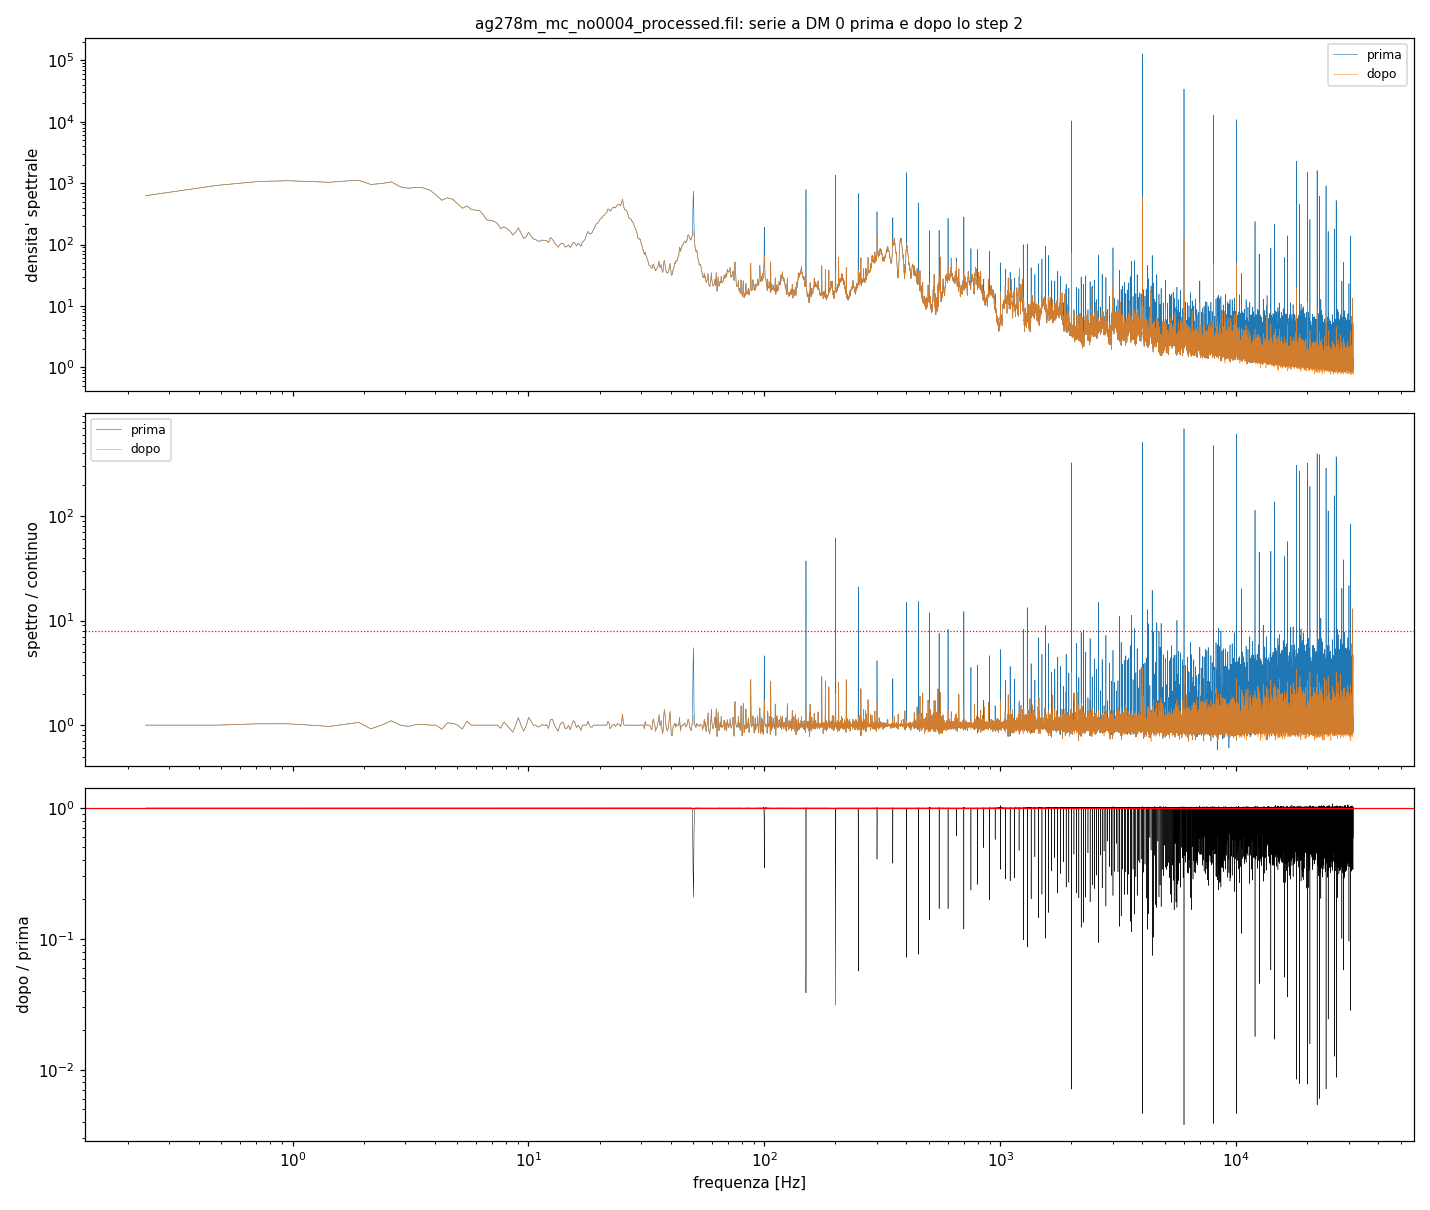
\includegraphics[width=0.9\textwidth]{fig/pipeline/step2_periodic_spectrum.png}
\caption{Step 2: spettro di potenza della serie a DM 0 a banda intera prima (blu) e dopo (arancione) la sottrazione
della famiglia a \SI{50}{\hertz}; in basso il rapporto dopo/prima. Le armoniche fino a \SI{30}{\kilo\hertz} sono ridotte
di un fattore tra 10 e 300.}
\label{fig:step2}
\end{figure}

\paragraph{Correzioni durante lo sviluppo.} L'arrotondamento deterministico annullava le correzioni inferiori a un
conteggio (da cui il dithering). Un profilo a 64 intervalli di fase, a gradini, creava righe fittizie (da cui la
risoluzione nativa in fase). Una presunta famiglia a \SI{166.67}{\hertz} era aliasing dello spettro decimato del
censimento (da cui lo spettro a risoluzione nativa). Una fondamentale sottomultipla rubava la riga a \SI{50}{\hertz}
di una pulsar sintetica (da cui l'interpolazione delle frequenze delle righe e la protezione delle famiglie non
testate).

% -------------------------------------------------------------------------------------
\FloatBarrier
\section{Step 3: impulsi a DM 0}
\label{sec:step3}

\paragraph{Metodo (versione finale).}
\begin{enumerate}
  \item \textbf{Rivelazione.} Serie a DM 0 della banda intera e di 16 sottobande, a rumore unitario. Boxcar da 1
    campione a \SI{32}{\milli\second}, con \textbf{soglia iterativa} (S/N 8, poi 6): la sigma robusta di ogni serie
    è ristimata escludendo i tratti già oltre soglia.
  \item \textbf{Un evento per impulso.} I rilevamenti sovrapposti nel tempo formano un gruppo; dentro il gruppo si
    prendono i boxcar in ordine di S/N decrescente, scartando quelli che si sovrappongono a uno già preso. Ogni impulso di
    un treno (radar) diventa così un evento separato.
  \item \textbf{Veto di dispersione.}
    \begin{itemize}
      \item Un evento più stretto di metà della dispersione a DM 15 nella serie in cui è visto non può essere un FRB a
        DM\,$\geq$\,15: è RFI senza altri calcoli.
      \item Altrimenti si cerca una traccia dispersa che passi per l'evento, su una griglia di DM (0--1000) e di larghezze
        (da $W/16$ a $2W$). L'evento è protetto se il miglior S/N a DM\,$\geq$\,15 supera di 1.05 volte quello a DM\,$<$\,15,
        è almeno 7, e lungo la traccia almeno il 40\% delle sottobande ha S/N\,$>$\,2. Per gli eventi a banda parziale si
        usano solo le sottobande non colpite.
      \item Se la traccia protetta non contiene, entro il proprio sweep, tutti gli altri impulsi a banda larga del
        gruppo, il veto è ripetuto con quegli impulsi azzerati: una traccia che attraversa impulsi diversi di un treno in
        sottobande diverse imita un FRB.
      \item Un evento che cade sulla traccia di un evento già protetto dello stesso gruppo è protetto anch'esso (i pezzi
        di un FRB visto a DM 0 in più sottobande).
    \end{itemize}
  \item \textbf{Sostituzione.} Il rettangolo tempo $\times$ sottobande colpite (tutti i canali se l'evento colpisce
    almeno metà delle sottobande), con un margine di $W/4$, è esteso finché le righe adiacenti hanno ancora segnale nelle
    sottobande sostituite (S/N\,$>$\,3.5 sulla serie combinata o $>$\,5 su una sottobanda): i bordi di un impulso possono
    essere sfasati tra sottobande. Il rettangolo è riempito con rumore gaussiano al livello del blocco, oppure al livello
    locale (media delle righe vicine senza eventi) se questo differisce significativamente ($z>5$), come per un impulso su
    un fondo rialzato. Tutti gli altri campioni restano identici.
\end{enumerate}

\paragraph{Evoluzione.} Lo step 3 è stato raffinato in quattro versioni, ciascuna verificata con la ricerca sul file
intero (Tab.~\ref{tab:step3}):
\begin{itemize}
  \item \textbf{v1}: sostituiva solo il boxcar migliore di ogni gruppo, quindi in un treno radar restava quasi tutto
    (nel passaggio del radar A a \SI{673.6}{\second} uno solo dei circa 20 impulsi). Il livello di sostituzione era la
    mediana del blocco, che su un fondo rialzato lasciava un ``buco'' con bordi netti: a \SI{568.709}{\second} questo
    buco generava un candidato nuovo con S/N 13.9.
  \item \textbf{v2}: un evento per impulso e livello locale. L'eccesso di candidati attorno al radar B scende da 100 a 33,
    ma i bordi degli impulsi sfasati tra le due metà della banda lasciavano ``schegge'' di 1--2 campioni (796 eventi a DM 0
    con S/N\,$\geq$\,10, il 91\% ai passaggi del radar A).
  \item \textbf{v3}: estensione dei rettangoli sui bordi (le schegge scendono a 14). Ma, ora che ogni impulso passava dal
    veto da solo, tracce disperse che collegavano impulsi diversi di un treno proteggevano 5856 eventi; e il livello
    locale, stimato con il primo quartile, era spostato verso l'alto di circa $0.3\sigma$ con treni densi, un errore che
    sommato su circa 250 canali crea nuovi impulsi.
  \item \textbf{v4} (finale): veto ripetuto con gli altri impulsi del treno azzerati e livello del blocco salvo
    differenze significative. Le protezioni scendono a 1221.
\end{itemize}

\begin{table}[ht]
\centering
\caption{Ricerca sul file intero (S/N\,$>$\,8, DM\,$>$\,28, cioè la selezione di produzione) dopo ciascuna versione
della pipeline. ``Radar A/B'': candidati entro la finestra dei passaggi radar (per caso circa il 4\%).
``Heimdall, tutti'': righe del file \file{.cand} completo.}
\label{tab:step3}
\small
\begin{tabular}{lrrrrrr}
\toprule
 & originale & step 1 (v. iniziale) & step 1+2 & +3 v1 & +3 v2 & \textbf{+3 v4} \\
\midrule
Candidati & 2399 & 816 & 749 & 591 & 341 & \textbf{338} \\
Heimdall, tutti & -- & 43184 & 42275 & 35021 & 28054 & \textbf{28344} \\
S/N\,$>$\,8 con DM\,$<$\,28 & -- & 109 & 96 & 77 & 36 & \textbf{10} \\
Stretti ($\leq2^3$ campioni) & 81\% & 16\% & 14\% & 10\% & 9\% & \textbf{4\%} \\
Attorno al radar A & 4.3\% & 7.6\% & 4.7\% & 5.4\% & 8.2\% & \textbf{4.4\%} \\
Attorno al radar B & 3.8\% & 19.6\% & 15.5\% & 16.9\% & 9.7\% & \textbf{7.4\%} \\
FETCH\,$\geq$\,0.7 & 0 & 2 & 0 & 1 & 0 & \textbf{0} \\
\bottomrule
\end{tabular}
\end{table}

\paragraph{Risultati della versione finale.} Su \SI{1199}{\second}: 72747 eventi a DM 0, 71526 rimossi (40698 con il
solo criterio di larghezza) e 1221 protetti; dati sostituiti 3.4\%; \SI{35}{\minute} di calcolo, di cui 9 nel veto.
Negli eventi a DM 0 del censimento, quelli con S/N\,$\geq$\,30 passano da 1105 (dopo lo step 2) a 8, e quelli tipici
dei radar (A: banda intera; B: metà bassa della banda) da 498 e 328 a 0; la frazione di tempo occupata da eventi scende
dal 6.3\% al 3.3\%. Il passaggio del radar A a \SI{673.6}{\second} è rimosso del tutto (Fig.~\ref{fig:radarA}).
L'unico candidato FETCH ``gold'' comparso con la v1 (\SI{657.412}{\second}, DM 45.8) era il bordo di un treno di
impulsi a banda stretta: con la v4 il treno è rimosso e il candidato scompare.

\begin{figure}[ht]
\centering
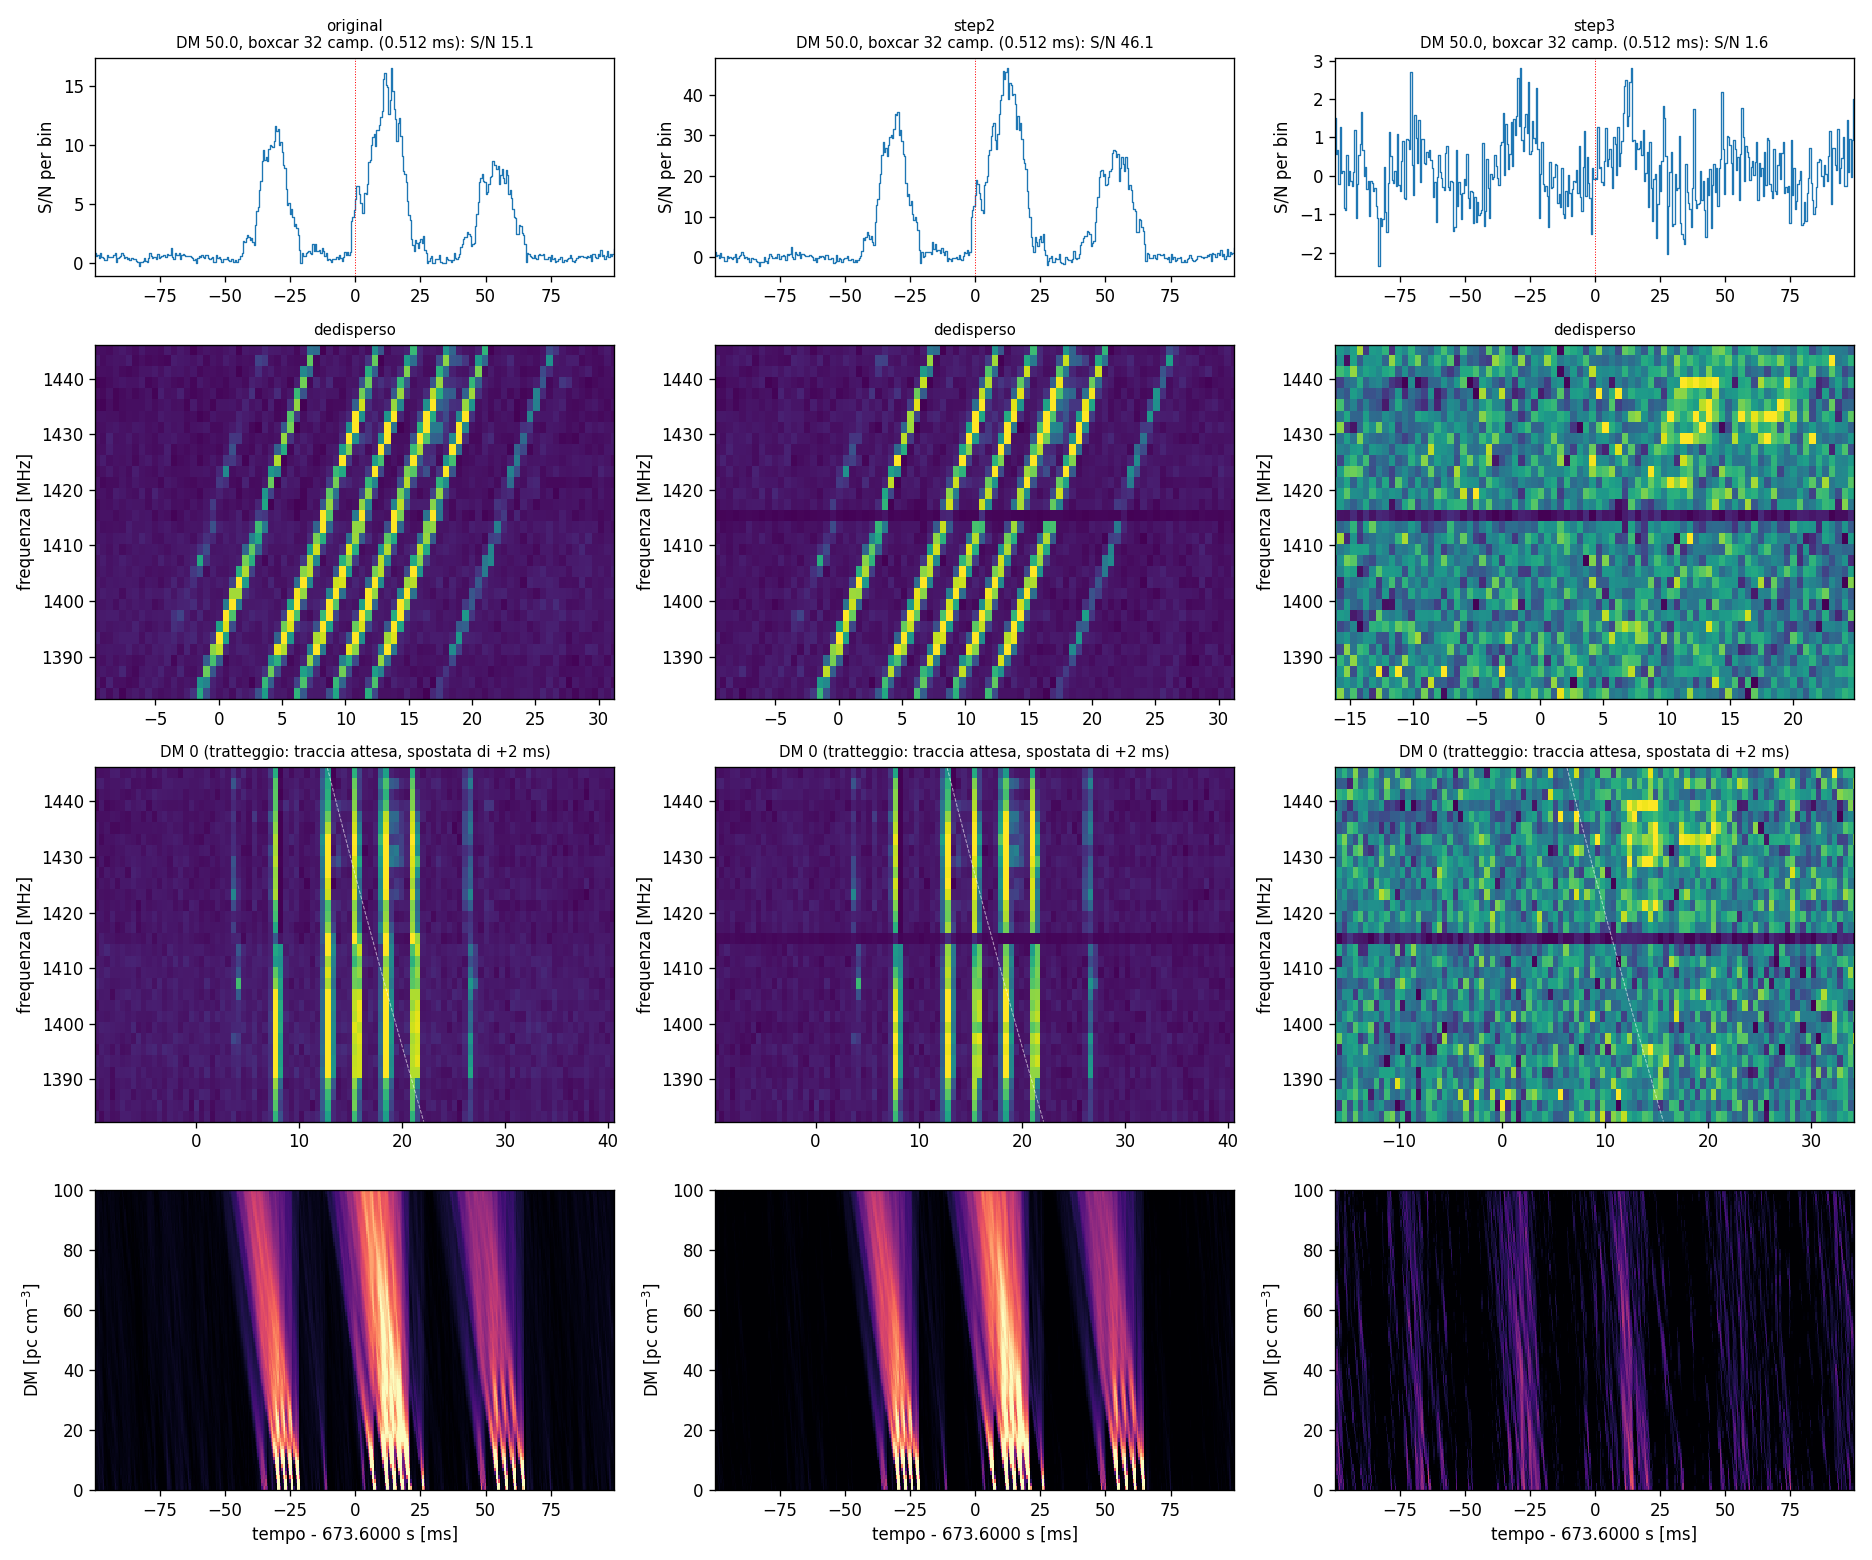
\includegraphics[width=\textwidth]{fig/pipeline/radarA_673_step3.png}
\caption{Passaggio del radar A a \SI{673.6}{\second}, mostrato con \file{tools/plot_cand.py} nel file originale, dopo
lo step 2 e dopo lo step 3 (v4). Dall'alto: profilo dedisperso a DM 50 (boxcar \SI{0.5}{\milli\second}), spettro
dinamico dedisperso, spettro dinamico a DM 0, piano DM--tempo. I tre gruppi di impulsi radar (S/N 46 dopo lo step 2)
spariscono dopo lo step 3 (S/N 1.6).}
\label{fig:radarA}
\end{figure}

\paragraph{Protezione degli FRB.} Su dati sintetici con radar e treni di impulsi, per FRB abbastanza brillanti da
essere visti anche a DM 0, il rapporto tra S/N dopo lo step 3 e S/N senza RFI è:
\begin{center}
\small
\begin{tabular}{lcccc}
\toprule
DM & \SI{0.5}{\milli\second} & \SI{1}{\milli\second} & \SI{4}{\milli\second} & \SI{16}{\milli\second} \\
\midrule
20 & 1.00 & 1.02 & 0.08 & 0.02 \\
30 & 1.00 & 1.00 & 1.00 & 0.05 \\
50 & 1.00 & 1.00 & 1.00 & 0.09 \\
100 & 0.97 & 1.00 & 1.00 & 1.00 \\
300 & 1.00 & 0.98 & 1.00 & 1.01 \\
\bottomrule
\end{tabular}
\end{center}
Il limite è fisico: un burst più largo di circa 0.7 volte il proprio sweep (\SI{5.6}{\milli\second} a DM 30,
\SI{9.4}{\milli\second} a DM 50) non è distinguibile da un impulso terrestre a DM 0. Gli FRB deboli, non rivelati a DM 0,
non vengono toccati. Sui treni sintetici densi e irregolari restano 1 impulso su 211 e nessuna protezione spuria.

% -------------------------------------------------------------------------------------
\FloatBarrier
\section{Step 4: rumore di modo comune}
\label{sec:step4}

\paragraph{Motivazione.} Il pilota della campagna di iniezione (Sez.~\ref{sec:completeness}) ha mostrato che, anche dopo
gli step 1--3, Heimdall misura sui dati reali circa metà dell'S/N atteso, mentre su rumore bianco con lo stesso
bandpass ne misura il 108\%. Il rapporto cresce con il DM (0.43 a DM 100, 0.62 a DM 400--700), come per un rumore comune
a tutti i canali che la dedispersione disperde tanto meglio quanto più lungo è lo sweep. Il censimento lo conferma: la
serie a DM 0 a banda intera ha un rumore 4.4 volte quello atteso per canali indipendenti su \SI{1}{\milli\second}, 11 volte
su \SI{16}{\milli\second} e 17 volte su \SI{65}{\milli\second}. È un rumore fortemente correlato tra i canali e
``rosso'', cioè dominante sulle scale lunghe.

\paragraph{Metodo.} Per ogni canale attivo, sui dati normalizzati $z_c=(x_c-\mu_c(t))/\sigma_c$,
\begin{equation}
z_c(t)=g_c\,m(t)+n_c(t),\qquad m(t)=\langle z_c(t)\rangle_c ,
\end{equation}
dove $m(t)$ è il modo comune (media su tutti i canali attivi) e $g_c$ l'accoppiamento del canale. L'output è
$x_c-\sigma_c g_c m(t)$.
\begin{itemize}
  \item $g_c$ è stimato per regressione di $z_c$ su $m$ in blocchi di \SI{4}{\second}, a risoluzione di
    \SI{1}{\milli\second}, con $m$ calcolato escludendo il canale stesso (altrimenti, con un modo comune debole, $g_c$
    tenderebbe a 1). Con \texttt{-{}-mode zerodm} si usa $g_c=1$ per tutti i canali (filtro a DM zero, Eatough et al.
    2009).
  \item Il livello $\mu_c(t)$ è la \emph{media} del canale nel blocco, interpolata linearmente tra i centri dei blocchi.
    Con la media il modo comune ha media nulla, quindi la sottrazione non introduce offset; con l'interpolazione il
    livello è continuo, quindi non introduce scalini tra i blocchi.
  \item Un FRB perde circa la frazione larghezza/sweep del proprio segnale: in ogni istante occupa solo quella frazione
    dei canali, che entra nella media. È trascurabile per i burst stretti ad alto DM (circa 2\% per \SI{1}{\milli\second}
    a DM 250), grande per quelli larghi a basso DM.
\end{itemize}

\paragraph{Validazione su dati sintetici} (modo comune rosso, accoppiamento variabile lungo la banda, eccesso di rumore
6 a DM 0). S/N di FRB senza modo comune, con modo comune e dopo lo step 4:
\begin{center}
\small
\begin{tabular}{lccc}
\toprule
 & solo rumore bianco & con modo comune & dopo step 4 \\
\midrule
\SI{1}{\milli\second}, DM 30--700 & 11.0--12.7 & 1.7--5.9 & 10.3--12.5 \\
\SI{4}{\milli\second}, DM\,$\geq$\,100 & 12.6--16.4 & 1.0--5.2 & 11.1--15.0 \\
\SI{16}{\milli\second}, DM 30--50 & 28.9--30.5 & 0.8--1.6 & 3.2--3.8 \\
\SI{16}{\milli\second}, DM 300--700 & 30.1--31.5 & 4.9--5.4 & 21.6--22.0 \\
\bottomrule
\end{tabular}
\end{center}
Su rumore bianco puro lo step 4 non cambia l'S/N (rapporto 0.94--1.02).

\paragraph{Risultati.} Sul tratto del pilota (\SIrange{500}{800}{\second}) l'eccesso di rumore a DM 0 su
\SI{1}{\milli\second} era 4.47. Gli accoppiamenti stimati hanno mediana 0.75 e una dispersione ampia (dal 10° al 90°
percentile: 0.36--1.70): un filtro a DM zero classico, con $g_c=1$, avrebbe sottratto troppo in alcuni canali e troppo
poco in altri. L'eccesso della differenza tra metà alta e metà bassa della banda scende solo da 2.48 a 2.03: resta una
parte correlata che un solo modo comune non descrive. Nel pilota lo step 4 porta i burst rivelati da 73 a 103 su 133 e
il rapporto tra S/N misurato e atteso da circa 0.5 a 0.85--0.92 (Sez.~\ref{sec:completeness}).

\paragraph{Una correzione importante.} La prima versione usava come livello del canale la \emph{mediana} del blocco.
Nei dati reali, a 8 bit e con una coda positiva di RFI residuo, la media di ogni canale supera la mediana di circa
$0.17\sigma$. Il modo comune aveva quindi in ogni blocco una media diversa da zero, che veniva sottratta moltiplicata
per $g_c$: uno scalino diverso per blocco e per canale. Lo spettro dinamico del file intero mostrava fasce larghe
qualche MHz e strisce verticali assenti prima (Fig.~\ref{fig:step4v1}); la struttura lenta per canale saliva del 46\%
(da $0.022\sigma$ a $0.033\sigma$ sulle medie a \SI{0.6}{\second}) e i salti tra intervalli successivi erano maggiori ai
confini dei blocchi. Con la media interpolata, su dati sintetici costruiti allo stesso modo, lo scalino introdotto tra
blocchi scende da $0.011\sigma$ a $0.0008\sigma$, e il recupero di S/N resta invariato. I risultati del pilota citati
sopra sono stati ottenuti con la prima versione e vanno ripetuti.

\begin{figure}[ht]
\centering
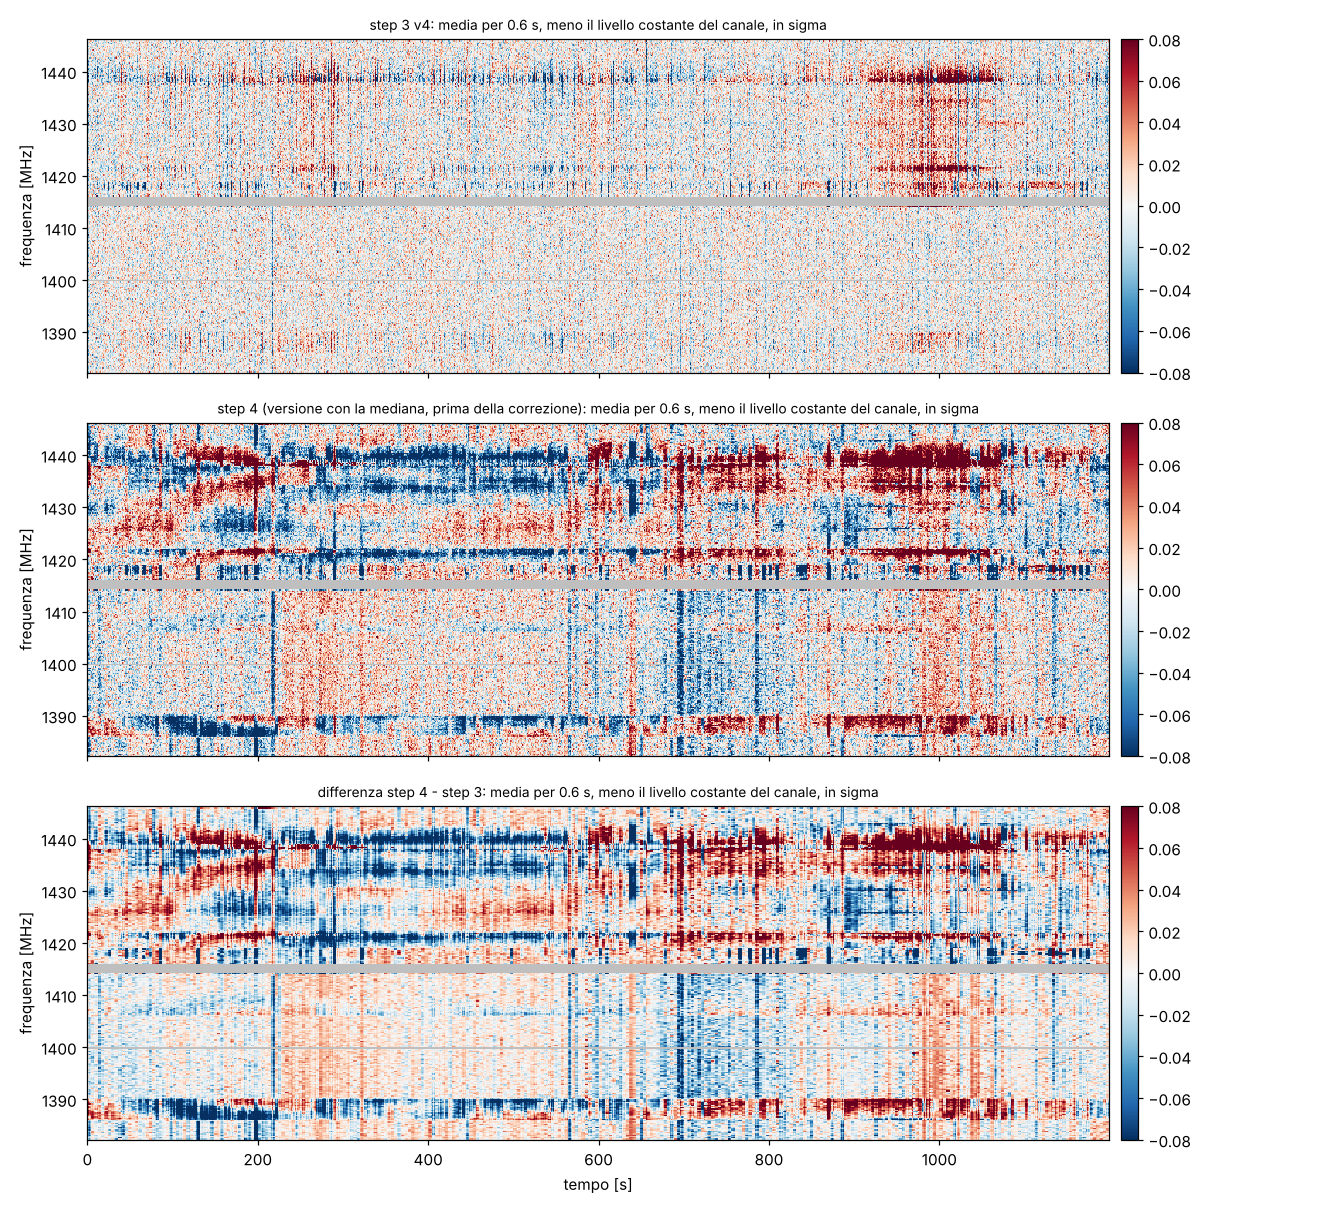
\includegraphics[width=\textwidth]{fig/pipeline/dynspec_step3_vs_step4v1.png}
\caption{Spettro dinamico del file intero (medie su \SI{0.6}{\second}, livello costante di ogni canale tolto) dopo lo
step 3, dopo la \emph{prima} versione dello step 4, e loro differenza. Le fasce e le strisce del pannello centrale sono
introdotte dallo step 4 (scalini per blocco e canale) e sono state eliminate nella versione attuale.}
\label{fig:step4v1}
\end{figure}

% -------------------------------------------------------------------------------------
\FloatBarrier
\section{Strumenti di diagnostica}
\label{sec:diag}

\begin{itemize}
  \item \file{tools/rfi_survey.py -{}-spectrum}: al censimento si aggiunge lo spettro di potenza della serie a DM 0
    (banda intera e 16 sottobande) e l'elenco delle righe con la loro famiglia armonica.
    \file{tools/compare_spectra.py} confronta due spettri e, per ogni riga, riporta la potenza rimasta.
  \item \file{tools/plot_cand.py}: ispezione di un candidato direttamente dal filterbank, su più file affiancati
    (profilo dedisperso, spettro dinamico dedisperso e a DM 0, piano DM--tempo). Le statistiche di canali e boxcar sono
    stimate su $\pm\SI{1}{\second}$, perché su finestre più corte l'S/N dei boxcar larghi risulta sottostimato.
  \item \file{tools/plot_dynspec.py}: spettri dinamici, serie temporali e spettri di uno o più file, uno sotto l'altro con
    lo stesso asse dei tempi; DM, finestra, risoluzione, numero di canali, unità (conteggi o $\sigma$) e colormap a scelta.
    È lo strumento della Fig.~\ref{fig:final}.
\end{itemize}

% -------------------------------------------------------------------------------------
\FloatBarrier
\section{Campagna di completezza: metodo e pilota}
\label{sec:completeness}

\paragraph{Metodo.} FRB sintetici vengono iniettati nel file \emph{originale}, poi si eseguono gli step 1--4 e la ricerca
di produzione dopo ogni step (\file{injection/run_realization.sh}). \file{injection/completeness_plan.py} prepara cinque
scansioni, mescolate a caso nel tempo, con almeno \SI{2}{\second} tra un burst e l'altro:
\begin{center}
\small
\begin{tabular}{llll}
\toprule
 & Varia & Fisso & Valori \\
\midrule
A & S/N & $w=\SI{1}{\milli\second}$, DM 250 & 5, 6, 7, 8, 9, 10, 12, 15, 20, 30 \\
B & larghezza, a flusso fisso & S/N$_{\rm 1ms}=20$, DM 250 & 0.1, 0.25, 0.5, 1, 2, 4, 8, 16, 32 ms \\
C & larghezza, a S/N fisso & S/N 20, DM 250 & come B \\
D & DM & $w=\SI{1}{\milli\second}$, S/N 20 & 30, 50, 75, 100, 150, 250, 400, 550, 700 \\
E & DM $\times$ larghezza & S/N 20 & DM 30, 50, 100 $\times$ 2, 4, 8, 16 ms \\
\bottomrule
\end{tabular}
\end{center}
Nella scansione B il flusso è espresso come S/N$_{\rm 1ms}$, l'S/N che il burst avrebbe se fosse largo \SI{1}{\milli\second}
allo stesso DM: l'ampiezza per canale resta fissa e l'S/N atteso segue la larghezza (50 a \SI{0.1}{\milli\second}, 20 a
\SI{1}{\milli\second}, 10 a \SI{4}{\milli\second}, 5 a \SI{16}{\milli\second}). La scansione C, a S/N fisso, separa le
perdite dovute alla pulizia da quelle dovute alla debolezza del burst. \file{injection/recover.py} associa candidati e
burst (scarto in tempo entro $\SI{20}{\milli\second}+2w$, in DM entro $\max(0.2\,\mathrm{DM},10)$) e produce, per ogni
step: la completezza con intervallo di Wilson al 68\%, il rapporto tra S/N di Heimdall e S/N atteso (anche sotto soglia, dal
file \file{.cand} completo), la frazione classificata da FETCH e i \textbf{falsi candidati per file}, divisi in
``vicini'' (rilevamenti spuri o doppi dei burst iniettati) e ``lontani''. Un file di solo rumore con lo stesso header e lo
stesso bandpass (\file{tools/make_noise_fil.py}) dà la completezza ideale e la calibrazione dell'S/N su Heimdall.

\paragraph{Pilota.} \SI{300}{\second} del file (\SIrange{500}{800}{\second}), scansioni A e D, 7 burst per punto
(133 burst). Gli scarti tra candidati e burst sono piccoli (mediana sotto \SI{0.1}{\milli\second} in tempo, $\pm3$ in
DM), quindi le tolleranze sono adeguate. Su rumore bianco Heimdall misura 1.08 volte l'S/N del modello dell'iniettore,
stabile da S/N 12 a 30 e a tutti i DM. Lo step 4 del pilota è la prima versione (Sez.~\ref{sec:step4}).

\begin{table}[ht]
\centering
\caption{Pilota, scansione A ($w=\SI{1}{\milli\second}$, DM 250): burst rivelati su 7 e, tra parentesi, mediana del
rapporto tra S/N di Heimdall e S/N atteso.}
\label{tab:pilotA}
\small
\begin{tabular}{lccccc}
\toprule
S/N iniettato & solo rumore & originale & step 1 & step 3 & step 4 \\
\midrule
8  & 7/7 (1.22) & 0/7 & 0/7 & 0/7 (0.94) & 3/7 (0.98) \\
9  & 7/7 (1.18) & 0/7 & 0/7 & 0/7 (0.73) & 3/7 (0.89) \\
10 & 7/7 (1.15) & 1/7 & 1/7 & 1/7 (0.77) & 6/7 (0.95) \\
12 & 7/7 (1.06) & 0/7 & 2/7 & 2/7 (0.56) & 7/7 (0.91) \\
15 & 7/7 (1.09) & 0/7 & 2/7 & 3/7 (0.69) & 7/7 (0.85) \\
20 & 7/7 (1.10) & 3/7 & 6/7 & 5/7 (0.47) & 7/7 (0.86) \\
30 & 7/7 (1.04) & 6/7 & 7/7 & 6/7 (0.62) & 7/7 (0.91) \\
\bottomrule
\end{tabular}
\end{table}

\begin{table}[ht]
\centering
\caption{Pilota: burst rivelati (su 133) e falsi candidati per file (\SI{300}{\second}). ``Vicini'': entro
\SI{0.5}{\second} più lo sweep da un burst iniettato. Nessun falso lontano ha probabilità FETCH\,$\geq$\,0.5.}
\label{tab:pilotfalse}
\small
\begin{tabular}{lrrrrr}
\toprule
 & selezionati & burst rivelati & falsi vicini & falsi lontani & S/N Heimdall / atteso (D) \\
\midrule
solo rumore & 162 & 117 & 24 & 21 & 1.04--1.11 \\
originale & 253 & 28 & 119 & 106 & 0.32--0.43 \\
step 1 & 264 & 67 & 91 & 106 & 0.42--0.60 \\
step 2 & 236 & 69 & 76 & 91 & 0.43--0.63 \\
step 3 & 162 & 73 & 38 & 51 & 0.43--0.62 \\
step 4 (prima versione) & 263 & 103 & 78 & 82 & 0.76--0.92 \\
\bottomrule
\end{tabular}
\end{table}

\begin{figure}[ht]
\centering
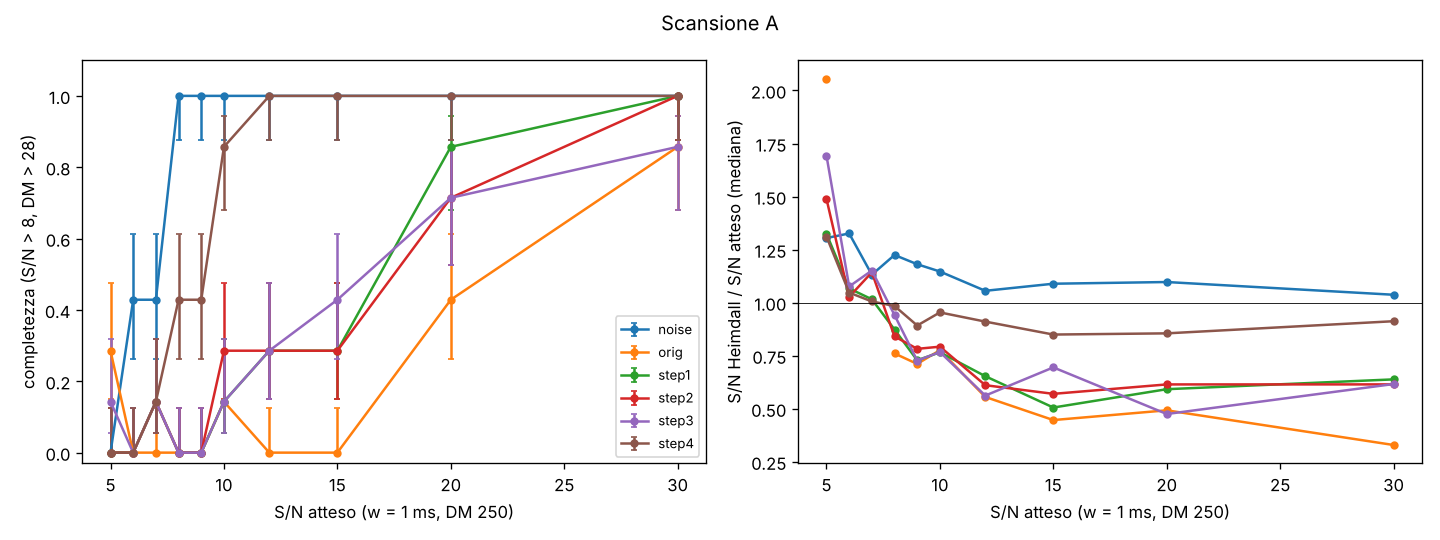
\includegraphics[width=\textwidth]{fig/pipeline/pilot_scan_A.png}\\
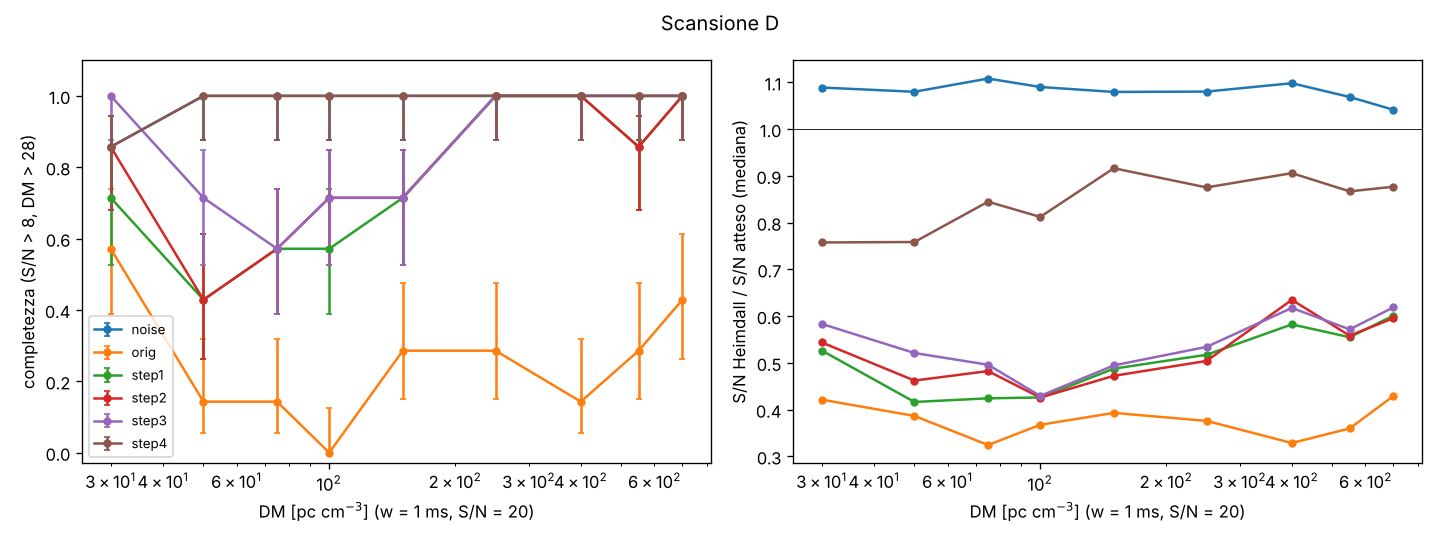
\includegraphics[width=\textwidth]{fig/pipeline/pilot_scan_D.png}
\caption{Pilota della campagna di completezza. In alto la scansione A (S/N variabile, $w=\SI{1}{\milli\second}$,
DM 250), in basso la scansione D (DM variabile, S/N 20). A sinistra la completezza (S/N\,$>$\,8, DM\,$>$\,28) con
intervalli di Wilson al 68\%, a destra il rapporto tra S/N di Heimdall e S/N atteso, per il file di solo rumore e dopo
ogni step.}
\label{fig:pilot}
\end{figure}

\paragraph{Lettura.}
\begin{itemize}
  \item Sul rumore bianco tutti i burst da S/N 8 in su sono rivelati. Sui dati reali, fino allo step 3, la soglia
    effettiva cade attorno a S/N iniettato 20: un burst a S/N 10 viene visto a circa 5--6. Con lo step 4 scende a circa 10.
  \item Il passo dall'originale allo step 1 vale un fattore 2.4 nei burst rivelati (da 28 a 67); lo step 4 un altro 40\%
    (da 73 a 103). Gli step 2 e 3 cambiano poco la completezza ma dimezzano i falsi lontani (da 106 a 51).
  \item Anche sul rumore bianco restano 21 falsi lontani in \SI{300}{\second}, tutti con boxcar di $2^{12}$--$2^{13}$
    campioni (\SIrange{65}{131}{\milli\second}): è un limite di Heimdall con \texttt{-{}-boxcar\_max 8192}, indipendente
    dalla pulizia.
  \item Lo step 4 (prima versione) aumenta i falsi lontani da 51 a 82, quasi tutti con boxcar di $2^{10}$--$2^{13}$
    campioni. 11 attraversano un confine di blocco da \SI{4}{\second}, contro circa 3 attesi per caso: una parte è dovuta
    agli scalini corretti nella versione attuale. \ipotesi{La parte restante è attribuita alla correlazione residua tra
    le due metà della banda, rossa, che Heimdall vede come eccessi a boxcar molto larghi; va verificato ripetendo il pilota
    con la versione attuale.}
\end{itemize}

% -------------------------------------------------------------------------------------
\FloatBarrier
\section{Risultato complessivo}
\label{sec:final}

La Fig.~\ref{fig:final} mostra, con \file{tools/plot_dynspec.py}, gli stessi \SI{10}{\second} dell'osservazione
(\SIrange{500.1}{510.1}{\second}) nel file originale e dopo ciascuno dei quattro step, a DM 0, risoluzione
\SI{0.5}{\milli\second} e 256 canali, in conteggi. Ogni pannello ha la propria scala di colori.
\begin{itemize}
  \item \textbf{Originale.} Il bandpass (spettro a destra) varia da circa 115 a 160 conteggi, con il minimo nei canali
    121--127. Blocchi di qualche centinaio di millisecondi più chiari o più scuri sono i salti di guadagno; i due gruppi di
    righe verticali a circa \SI{3.5}{\second} e \SI{5.9}{\second} sono passaggi del radar A (\SI{503.65}{\second}, entro
    \SI{45}{\milli\second} dalla fase prevista) e del radar B (\SI{505.95}{\second}, nella metà bassa della banda). Sono
    visibili anche brevi impulsi a banda stretta a \SIrange{1415}{1420}{\mega\hertz} e l'emissione persistente a
    \SIrange{1438}{1440}{\mega\hertz}.
  \item \textbf{Step 1.} Il bandpass è reso piatto (circa 128 conteggi), i salti di guadagno sono normalizzati e i canali
    121--127 e 185 mascherati (grigio). Gli impulsi radar restano: la serie temporale li mostra ancora a 135--145 conteggi.
  \item \textbf{Step 2.} Differenze minime a questa scala: la sottrazione della famiglia a \SI{50}{\hertz} agisce su
    scale di \SI{20}{\milli\second} e inferiori.
  \item \textbf{Step 3.} I due passaggi radar spariscono dalla serie temporale e dallo spettro dinamico; restano le
    variazioni a banda larga del modo comune, ben visibili nella serie temporale (circa $\pm1$ conteggio, contro un rumore
    bianco atteso di circa 0.09 conteggi per bin).
  \item \textbf{Step 4.} La serie temporale è ridotta a circa $\pm0.1$ conteggi: a DM 0 la componente comune è sottratta
    per costruzione, quindi questa serie non va confrontata con il rumore bianco, ma mostra che il modo comune è stato
    rimosso a tutte le scale fino a qualche secondo. Lo spettro dinamico non ha più strisce verticali; restano piccoli residui a
    \SI{1440}{\mega\hertz} (emissione a banda stretta) e attorno a \SI{3.9}{\second}, in corrispondenza della fine di un
    salto di guadagno.
\end{itemize}

\begin{figure}[p]
\centering
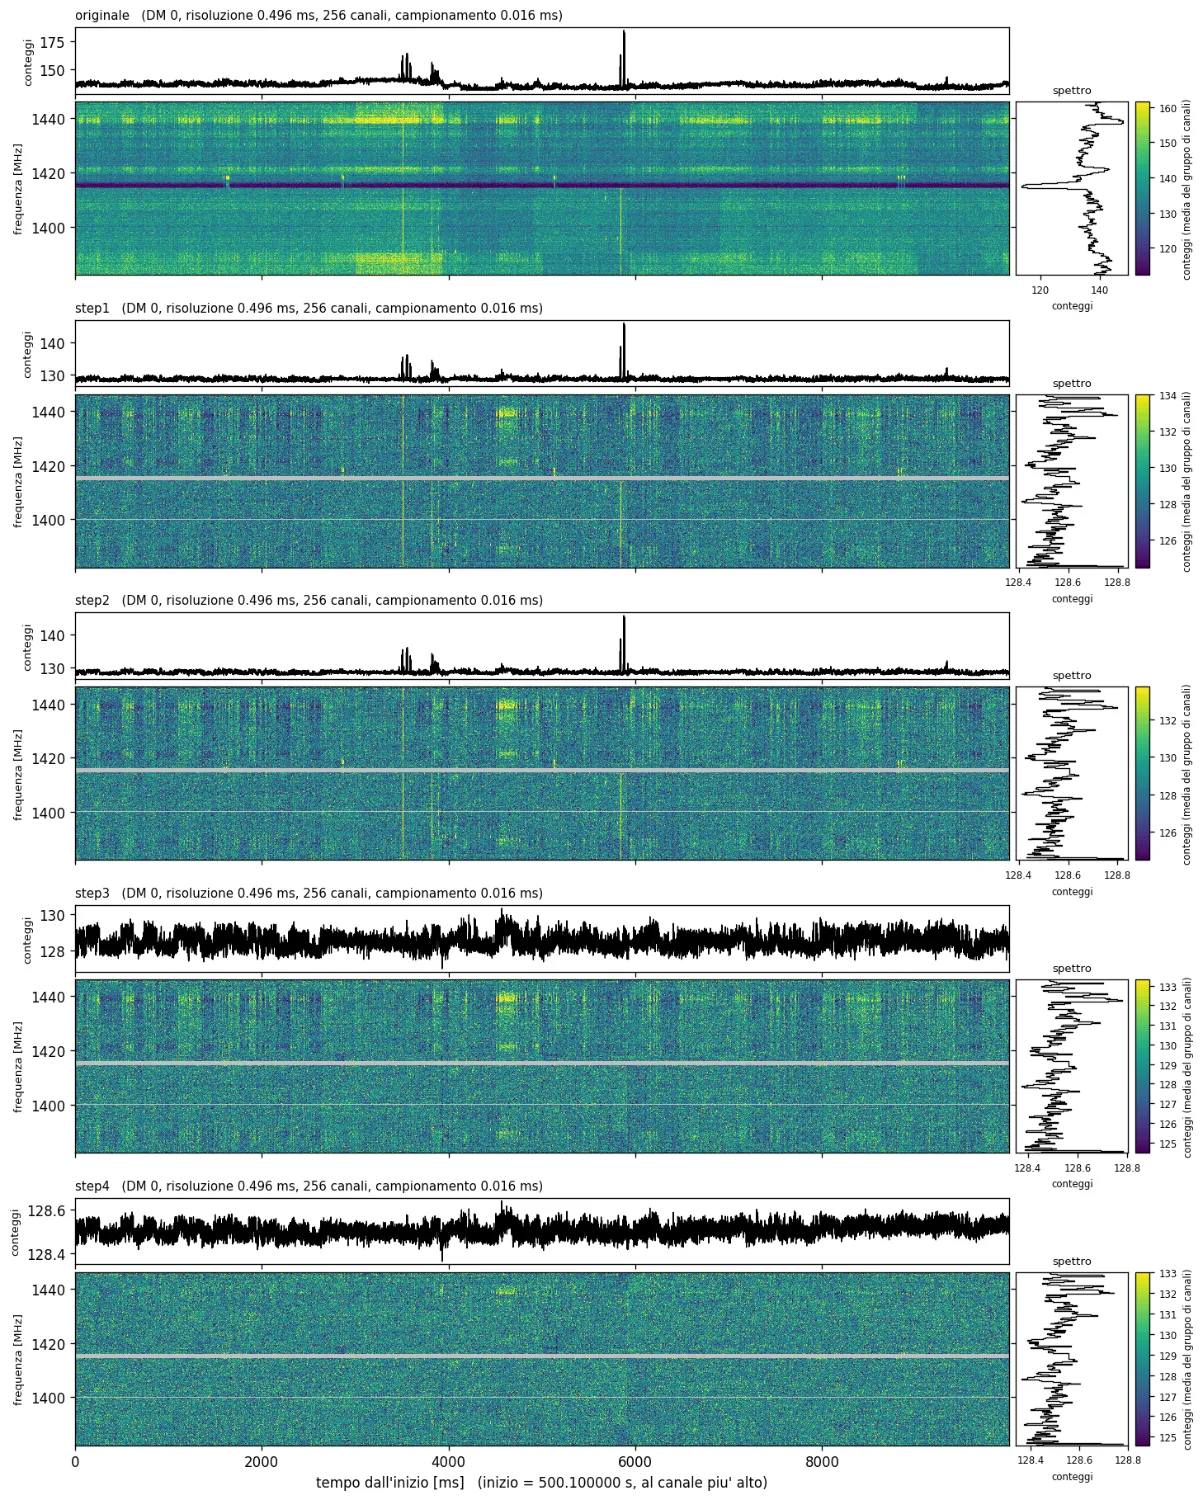
\includegraphics[width=\textwidth,height=0.88\textheight,keepaspectratio]{fig/pipeline/steps_500s.png}
\caption{\SI{10}{\second} dell'osservazione (da \SI{500.1}{\second}) nel file originale e dopo gli step 1, 2, 3 e 4
(dall'alto in basso), con \file{tools/plot_dynspec.py}: per ciascuno la serie temporale (media dei conteggi su tutti i
canali attivi), lo spettro dinamico a DM 0 (risoluzione \SI{0.5}{\milli\second}, 256 canali) e lo spettro medio sulla
finestra. Grigio: canali mascherati. Ogni pannello ha la propria scala di colori e il proprio asse delle serie temporali.}
\label{fig:final}
\end{figure}

% =====================================================================================
% Caratterizzazione dell'ambiente RFI di Medicina in banda L (incluso da pipeline.tex)
% =====================================================================================
\FloatBarrier
\section{L'ambiente RFI di Medicina in banda L}
\label{sec:rfienv}

Questa sezione riassume ciò che le analisi precedenti dicono dell'ambiente di interferenze e del rumore del sistema,
indipendentemente dalla pipeline. Si basa su due osservazioni con lo stesso setup
(\SIrange{1382.25}{1446.25}{\mega\hertz}, 256 canali da \SI{0.25}{\mega\hertz}, \SI{16}{\micro\second}, 8 bit):
\begin{itemize}
  \item \file{ag278m_mc_no0004} (\SI{1199}{\second}, campo di un transiente, Sez.~\ref{sec:results} e seguenti);
  \item \file{ag293m_mc_no0001} (\SI{179}{\second}, puntamento su B0329+54).
\end{itemize}
I filterbank sono già limitati a \SI{64}{\mega\hertz}: la banda del ricevitore è più ampia, ma è stata tagliata a
monte a causa di RFI persistente molto forte. Anche la tabella delle prestazioni dell'antenna indica a
\SI{1.4}{\giga\hertz} una banda utile ridotta ($2\times\SI{80}{\mega\hertz}$) per le interferenze.

% -------------------------------------------------------------------------------------
\subsection{Tipi di interferenza}

\begin{table}[ht]
\centering
\caption{Inventario delle interferenze nelle due osservazioni, dai censimenti (\file{rfi_survey.py}) e dai
riassunti degli step della pipeline.}
\label{tab:rfienv}
\small
\begin{tabular}{p{3.3cm}p{5.6cm}p{5.6cm}}
\toprule
 & \file{ag278m_mc_no0004} (\SI{1199}{\second}) & \file{ag293m_mc_no0001} (\SI{179}{\second}) \\
\midrule
Canali inutilizzabili (maschera dello step 1) & 8: 121--127 (\SIrange{1414.4}{1415.9}{\mega\hertz}) e 185
  (\SI{1399.9}{\mega\hertz}) & 20: 0, 85, 140--145, 185, 200--205, 240--244 (gruppi a \num{1409.9}--\num{1411.1},
  \num{1394.9}--\num{1396.1}, \num{1385.1}--\SI{1386.1}{\mega\hertz}), con curtosi anomala \\
Salti di guadagno a banda larga & 1366 (\SI{1.1}{\per\second}), più forti ai bordi della banda & 65
  (\SI{0.36}{\per\second}) \\
Rete elettrica & \SI{50.0000006}{\hertz} e 55 armoniche fino a \SI{30}{\kilo\hertz}; 45.8\% della varianza della serie a
  DM 0 & \SI{50.000004}{\hertz}, 21 armoniche \\
Radar & due sorgenti con periodo \SI{10.0}{\second}: A a banda intera, B nella metà bassa; passaggi di circa
  \SI{90}{\milli\second} con treni di impulsi da \SI{0.5}{\milli\second} ogni \SIrange{2}{3}{\milli\second}, fino a
  S/N 120 a DM 0 & presenti con la stessa struttura (es. \SIrange{0.91}{0.955}{\second}) \\
Impulsi periodici rettangolari & -- & periodo \SI{0.50334}{\second} (\SI{1.987}{\hertz}), larghi
  \SI{8.5}{\milli\second}, non dispersi, simultanei in tutti i canali, più forti nei canali bassi: 356 su 356 periodi
  \\
Emissione a banda stretta persistente & \SIrange{1436}{1440}{\mega\hertz}, \SIrange{1420}{1422}{\mega\hertz},
  \SIrange{1387}{1390}{\mega\hertz}, variabile su decine di secondi; impulsi brevi a \SIrange{1415}{1420}{\mega\hertz}
  & -- (non analizzata) \\
Eventi impulsivi a DM 0 (step 3) & 72747 (\SI{61}{\per\second}); 3.4\% dei dati sostituiti & 10381
  (\SI{58}{\per\second}); 3.2\% dei dati sostituiti \\
\bottomrule
\end{tabular}
\end{table}

Alcune osservazioni:
\begin{itemize}
  \item \textbf{Il tasso di eventi impulsivi a DM 0 è lo stesso nelle due osservazioni} (circa 60 al secondo), mentre
    canali cattivi e salti di guadagno cambiano molto. Gli impulsi sembrano una caratteristica stabile del sito; canali
    e guadagno dipendono dalla sessione.
  \item \textbf{Gli impulsi periodici a \SI{1.987}{\hertz}} di \file{ag293m} sono stati inizialmente scambiati per la
    pulsar. Lo spettro dinamico a DM 0 mostra però bordi di salita e discesa simultanei in tutti i canali, e dedispersi a
    DM 26.7 si inclinano: non sono dispersi. \ipotesi{La forma rettangolare e la periodicità rigorosa suggeriscono
    un'apparecchiatura che commuta periodicamente.}
  \item \textbf{I radar} sono il disturbo impulsivo più intenso. Nella ricerca di \file{ag278m} sono stati la principale
    sorgente di candidati spuri dopo lo step 1 (Tab.~\ref{tab:step3}).
\end{itemize}

% -------------------------------------------------------------------------------------
\subsection{Rumore correlato tra i canali}

In entrambe le osservazioni il rumore della serie a DM 0 a banda intera è molto superiore a quello atteso per canali
indipendenti, e cresce con la scala di tempo: un rumore comune a tutti i canali e ``rosso''.
\begin{center}
\small
\begin{tabular}{lcc}
\toprule
 & \file{ag278m_mc_no0004} & \file{ag293m_mc_no0001} \\
\midrule
Rumore a DM 0 / atteso, su \SI{1}{\milli\second} (dopo lo step 3) & 4.4 (pilota: 4.47) & 4.74 \\
Idem su \SI{16}{\milli\second} / \SI{65}{\milli\second} & 11 / 17 & -- \\
Correlazione residua tra metà alta e metà bassa della banda & 2.48 & 2.52 \\
Accoppiamento dei canali al modo comune (mediana; 10°--90° percentile) & 0.75 (0.36--1.70) & 0.71 (0.46--1.88) \\
\bottomrule
\end{tabular}
\end{center}
I valori sono quasi identici nelle due osservazioni: il rumore correlato è una proprietà stabile del sistema, non un
episodio. L'accoppiamento varia molto da canale a canale, e una parte della correlazione (la differenza tra le due metà
della banda) non è descritta da un solo modo comune.

% -------------------------------------------------------------------------------------
\subsection{Sensibilità: B0329+54}
\label{sec:b0329}

\paragraph{Prestazioni nominali.} Dal manuale dell'antenna (Tab.~5.2, a \ang{45} di elevazione): a
\SI{1.4}{\giga\hertz} $T_{\rm sys}=\SI{58}{\kelvin}$, $G=\SI{0.120}{\kelvin\per\jansky}$, efficienza 41\%, da cui
$\text{SEFD}=T_{\rm sys}/G\simeq\SI{483}{\jansky}$ per polarizzazione.

\paragraph{Metodo.} Il file \file{ag293m_mc_no0001} è stato ripiegato con \file{prepfold} al periodo
\SI{0.71452}{\second} e DM 26.76, 128 intervalli di fase, dopo ogni step della pipeline. L'S/N del profilo è misurato
come segnale integrato sui 6 intervalli dell'impulso (circa \SI{34}{\milli\second}) diviso il rumore robusto fuori
dall'impulso. Il $\chi^2$ di \file{prepfold} non è adatto al confronto: presuppone rumore bianco ed è gonfiato dal
rumore correlato (da 1438 nell'originale a 4.9 dopo lo step 4, ma per la riduzione del rumore, non del segnale).

\paragraph{Rumore radiometrico.} Dopo lo step 1 ogni canale ha rumore $\sigma=8$ conteggi, quindi il rumore bianco
atteso per intervallo di fase è $8\sqrt{N_{\rm canali}}\sqrt{N_{\rm campioni/bin}}=8\sqrt{236}\sqrt{86400}\simeq
\num{3.6e4}$ conteggi. Il rumore misurato fuori impulso è 6.7--7.2 volte questo valore negli step 1--3 e 1.4 volte
dopo lo step 4. Rispetto al rumore radiometrico la pulsar ha S/N\,$\simeq$\,172; rispetto a quello reale circa 25.

\begin{table}[ht]
\centering
\caption{B0329+54 dopo ogni step: S/N del profilo rispetto al rumore reale, rapporto tra rumore reale e radiometrico,
segnale integrato rispetto allo step 2.}
\label{tab:b0329}
\small
\begin{tabular}{lcccc}
\toprule
 & S/N del picco & S/N integrato & rumore / radiometrico & segnale / step 2 \\
\midrule
originale & 19.4 & 24.9 & -- & -- \\
step 1 & 19.1 & 23.7 & 7.2 & 1.00 \\
step 2 & 20.8 & 25.7 & 6.7 & 1.00 \\
step 3 & 16.9 & 21.7 & 7.3 & 0.92 \\
step 4 & 12.6 & 8.8 & 1.4 & 0.07 \\
\bottomrule
\end{tabular}
\end{table}

\paragraph{Flusso e SEFD.} Con l'equazione del radiometro,
\begin{equation}
S_{\rm media}=\frac{\text{SEFD}}{\sqrt{n_{\rm pol}\,\Delta\nu\,\tau_{\rm bin}}}\cdot
\frac{\text{S/N}_{\rm int}\sqrt{N_{\rm on}}}{N_{\rm bin}},
\end{equation}
con $\Delta\nu=\SI{59}{\mega\hertz}$ (canali attivi), $\tau_{\rm bin}=\SI{176.9}{\second}/128$, $N_{\rm on}=6$,
$N_{\rm bin}=128$ e lo S/N radiometrico, si ottiene $S_{\rm media}\simeq \text{SEFD}\times\num{2.6e-4}$ per
$n_{\rm pol}=2$ e $\text{SEFD}\times\num{3.7e-4}$ per $n_{\rm pol}=1$. Con la SEFD nominale:
\begin{center}
\small
\begin{tabular}{lccc}
\toprule
Polarizzazioni nel file & $S_{\rm media}$ misurato & rapporto con il catalogo ($\simeq\SI{203}{\milli\jansky}$) &
  S/N radiometrico atteso \\
\midrule
2 & $\simeq\SI{125}{\milli\jansky}$ & 0.62 & $\simeq280$ \\
1 & $\simeq\SI{175}{\milli\jansky}$ & 0.87 & $\simeq200$ \\
\bottomrule
\end{tabular}
\end{center}
Viceversa, il flusso di catalogo implica una SEFD effettiva di circa \SI{790}{\jansky} ($n_{\rm pol}=2$) o
\SI{560}{\jansky} ($n_{\rm pol}=1$). Le incertezze principali sono la scintillazione di B0329+54 in banda L (il flusso in
un dato giorno può discostarsi dal valore di catalogo del 30--50\%), l'elevazione (la tabella vale a \ang{45}), il
puntamento e il numero di polarizzazioni nel file, da confermare. \ipotesi{Il flusso di catalogo è citato a memoria
(ATNF, $S_{1400}$) e va verificato.}

\paragraph{Lettura.}
\begin{itemize}
  \item \textbf{La SEFD del sistema è compatibile con quella nominale} entro un fattore 1.2--1.6, cioè entro le
    incertezze: non c'è indicazione di un ricevitore che renda meno del previsto. Il taglio a \SI{64}{\mega\hertz} non
    cambia la SEFD (grandezza per unità di banda) ma solo $\Delta\nu$. \ipotesi{L'RFI forte fuori dalla banda
    conservata potrebbe però aumentare $T_{\rm sys}$ nei canali rimasti, per compressione o intermodulazione
    nell'elettronica o per i fianchi dei filtri: un aumento della SEFD effettiva di questo tipo non è distinguibile, con
    questi dati, dalla scintillazione.}
  \item \textbf{La perdita di sensibilità viene dal rumore correlato}, non dalla SEFD: il profilo ripiegato è circa 7
    volte più rumoroso del limite radiometrico (S/N 25 invece di circa 170 in \SI{177}{\second}). Lo stesso fattore si
    ritrova, sulle scale dei millisecondi, nella serie a DM 0 di entrambe le osservazioni e nel pilota della campagna
    di completezza.
  \item \textbf{Effetto della pipeline sulla pulsar} (Tab.~\ref{tab:b0329}, Fig.~\ref{fig:b0329}): gli step 1 e 2 non
    perdono segnale; lo step 3 ne conserva il 92\% (rimuove alcuni impulsi singoli brillanti, visti a DM 0); lo step 4 ne
    conserva solo il 7\% e deforma il profilo. L'impulso di B0329+54 (circa \SIrange{6}{7}{\milli\second}) è più largo
    del proprio sweep su \SI{64}{\mega\hertz} (\SI{5}{\milli\second}), quindi in ogni istante è presente in quasi tutti i
    canali e viene sottratto come modo comune: è il limite larghezza/sweep previsto (Sez.~\ref{sec:step4}), qui confermato
    su dati reali.
\end{itemize}

\begin{figure}[ht]
\centering
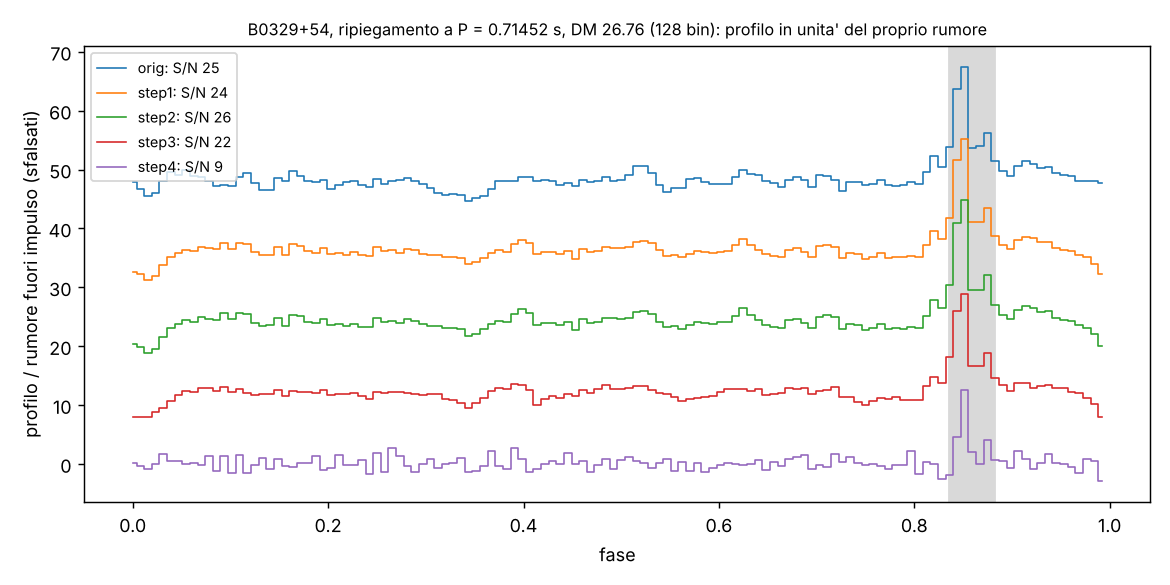
\includegraphics[width=0.85\textwidth]{fig/pipeline/B0329_profiles.png}
\caption{Profili di B0329+54 (\file{ag293m_mc_no0001}, \SI{177}{\second}, 128 intervalli) nel file originale e dopo
ogni step, ciascuno in unità del proprio rumore fuori impulso e sfalsati in verticale. In grigio la finestra
dell'impulso usata per l'S/N.}
\label{fig:b0329}
\end{figure}

\begin{figure}[ht]
\centering
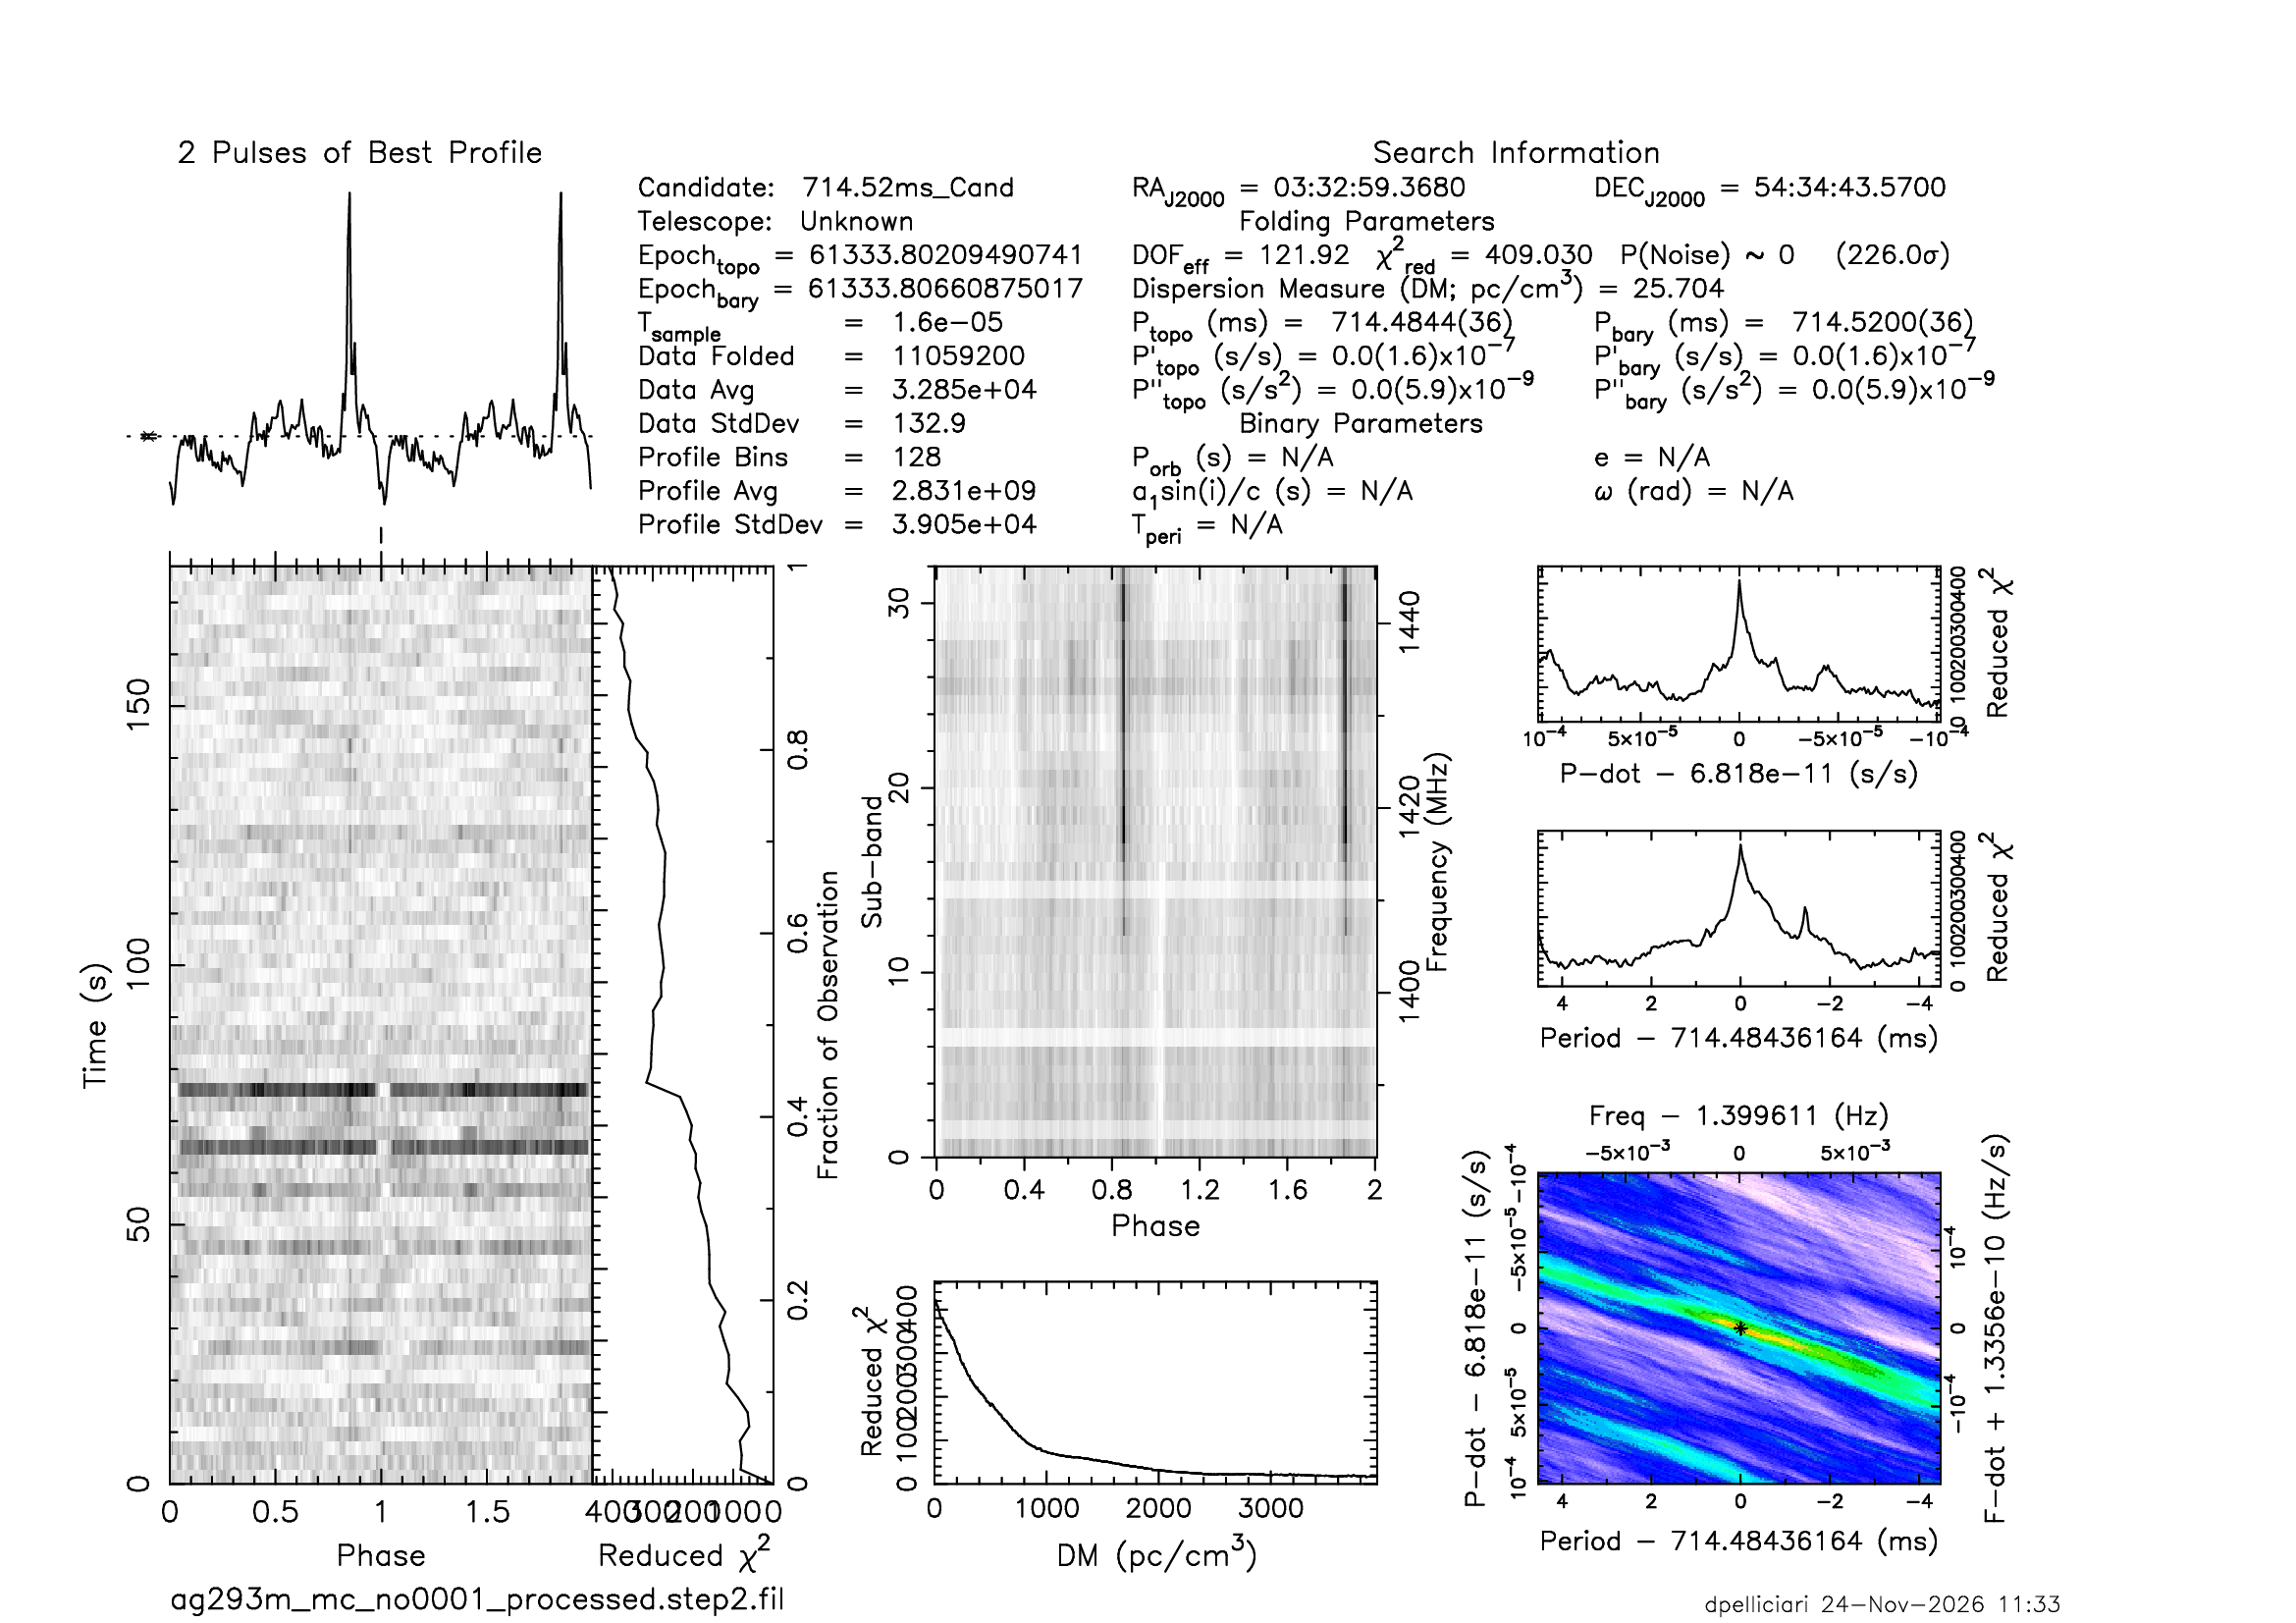
\includegraphics[width=0.95\textwidth]{fig/pipeline/B0329_prepfold_step2.png}
\caption{Ripiegamento di \file{prepfold} dopo lo step 2 (B0329+54, $P=\SI{0.71452}{\second}$, DM 26.76): profilo,
fase--tempo, fase--sottobanda e curve di $\chi^2$. Il $\chi^2$ riportato è gonfiato dal rumore correlato e non misura la
forza della pulsar (vedi testo).}
\label{fig:b0329pfd}
\end{figure}

% -------------------------------------------------------------------------------------
\subsection{Indicazioni per il sistema}
\begin{enumerate}
  \item Il guadagno in sensibilità più grande non verrebbe dalla pulizia a valle, ma dall'eliminazione del
    \textbf{rumore correlato tra i canali}, che costa un fattore circa 7 sui segnali impulsivi e ripiegati. Le possibili
    origini da verificare: elettronica di conversione, digitalizzazione, un controllo automatico del guadagno o
    un'altra regolazione a valle (compatibile con i salti di guadagno a intervalli di circa \SI{1}{\second}),
    interferenze a banda larga.
  \item Confermare con i tecnici: numero di polarizzazioni nei filterbank, elevazione durante le osservazioni, presenza
    di regolazioni automatiche del guadagno.
  \item Identificare le sorgenti locali: i due radar con periodo di \SI{10}{\second}, l'apparecchiatura a
    \SI{1.987}{\hertz}, l'emissione persistente a \SIrange{1436}{1440}{\mega\hertz} e \SIrange{1420}{1422}{\mega\hertz}.
  \item Ripetere la misura su B0329+54 in più giorni, per separare la scintillazione da eventuali variazioni del
    sistema, e con un calibratore nella stessa sessione per una SEFD assoluta.
\end{enumerate}

% -------------------------------------------------------------------------------------
\FloatBarrier
\section{Test su dati reali: la Crab osservata a Noto}
\label{sec:crabnoto}

Il test su B0329+54 (Sez.~\ref{sec:b0329}) riguarda un segnale lento e poco disperso, il caso sfavorevole per gli step 3 e
4. La pulsar della Crab (B0531+21, DM 56.7) è il caso opposto e il più vicino a un FRB: emette \emph{impulsi giganti}
singoli, stretti (decine di microsecondi) e fortemente dispersi. Il test usa anche un'antenna e un setup diversi da
quelli su cui la pipeline è stata sviluppata, quindi verifica pure che i valori di default non siano adattati a Medicina.

\subsection{Dati e pulizia}
Il file \file{n0325e_nt_no0005_IFall_vdif_pol2.fil} (Noto, 18 febbraio 2025) ha 1024 canali da \SI{0.25}{\mega\hertz}
(\SIrange{1350}{1606}{\mega\hertz}), campionamento di \SI{4}{\micro\second}, 8 bit e \SI{294}{\second} di durata
(\SI{75}{\giga\byte}). A DM 56.7 la dispersione attraversa la banda in circa \SI{38}{\milli\second}. La pipeline
(\file{tools/rfi_pipeline.py}, step 1--4, opzioni di default) ha impiegato \SI{4.7}{\hour}:
\begin{itemize}
  \item \textbf{step 1}: 100 canali mascherati, soprattutto il blocco \SIrange{1453}{1471}{\mega\hertz} (canali
    540--611, curtosi alta: RFI impulsivo), una ventina di canali a \SIrange{1521}{1563}{\mega\hertz} e alcuni a
    \SIrange{1364}{1382}{\mega\hertz}; 171 salti di guadagno; 0.03\% delle celle sostituite;
  \item \textbf{step 2}: una famiglia periodica a \SI{12.5}{\hertz} con 44 armoniche, sottratta;
  \item \textbf{step 3}: 9599 impulsi a DM 0, tutti rimossi, nessuno protetto; 1.7\% dei dati sostituiti;
  \item \textbf{step 4}: eccesso di rumore a DM 0 da 3.55 a 0.19 (a Medicina era 4.4--4.7), guadagno mediano 0.92.
    L'eccesso della differenza tra le due metà della banda resta 2.1: anche qui una parte della correlazione non è
    descritta da un solo modo comune.
\end{itemize}

\subsection{Impulsi giganti}
Il file originale e quello pulito sono stati cercati con \file{FRB_HF_Finder.py} (Heimdall + FETCH, DM 25--700,
soglia S/N 8, boxcar fino a 8192 campioni, modello \file{a}).

\paragraph{Identificazione dalla fase.} Per riconoscere gli impulsi giganti senza dipendere dalle soglie si usa la
periodicità della pulsar. I 30 candidati del file pulito con DM $56.72\pm0.2$ e FETCH\,$\geq$\,0.5 sono stati ripiegati
in tempo su una griglia di periodi (\SIrange{33.80}{33.88}{\milli\second}), massimizzando la statistica $Z^2_5$. Il
periodo topocentrico che li mette in fase è $P=\SI{33.84143}{\milli\second}$ ($Z^2_5=257$, contro 13 in mediana sulla
griglia): con questo periodo 28 impulsi cadono entro $\pm0.015$ in fase (impulso principale) e 2 a $+0.40$
(interimpulso), come atteso per la Crab (Fig.~\ref{fig:crabnoto}, a sinistra). Il periodo baricentrico corrispondente,
circa \SI{33.838}{\milli\second}, è coerente con la rotazione della Crab estrapolata a febbraio 2025.
\ipotesi{Il confronto con l'effemeride usa valori di frequenza e derivata citati a memoria; va verificato con
l'effemeride mensile di Jodrell Bank.} Si conta come impulso gigante ogni candidato con DM entro 1 da 56.72 e fase
entro 0.03 dall'impulso principale o dall'interimpulso: a quella DM, fuori fase, c'è un solo candidato per file.

\begin{table}[ht]
\centering
\caption{Ricerca con \file{FRB_HF_Finder.py} sul file originale e su quello pulito (step 1--4).}
\label{tab:crabnoto}
\small
\begin{tabular}{lcc}
\toprule
 & originale & pulito \\
\midrule
candidati Heimdall (DM 25--700) & 575 & 338 \\
impulsi giganti (in fase, DM $56.72\pm1$) & 28 & \textbf{43} \\
\quad di cui con FETCH\,$\geq$\,0.5 & 13 & \textbf{30} \\
candidati che non sono la Crab & 547 & 295 \\
\quad a DM 25--50 & 124 & 55 \\
\quad con boxcar $\geq2^{12}$ campioni & 157 & 263 \\
\quad con FETCH\,$\geq$\,0.5 & 0 & 0 \\
\midrule
impulsi giganti in comune & \multicolumn{2}{c}{26} \\
S/N pulito / originale (mediana; intervallo) & \multicolumn{2}{c}{1.17;\; 0.91--2.06} \\
\bottomrule
\end{tabular}
\end{table}

\paragraph{Risultati} (Tab.~\ref{tab:crabnoto}, Fig.~\ref{fig:crabnoto}).
\begin{itemize}
  \item \textbf{Più impulsi rivelati.} Gli impulsi giganti passano da 28 a 43, quelli accettati da FETCH da 13 a 30.
    Dei 28 dell'originale, 26 sono trovati anche nel file pulito; i 2 persi sono vicini alla soglia (S/N 8.3--8.4) e
    FETCH li scartava già. Dopo la pulizia compaiono 17 impulsi nuovi.
  \item \textbf{Nessuna perdita di segnale.} Per i 26 impulsi in comune l'S/N migliora in mediana del 17\%, senza casi
    di perdita significativa (minimo 0.91). Lo step 3 non ha protetto nessun evento e non ha comunque toccato gli
    impulsi: lo sweep di \SI{38}{\milli\second} li distingue nettamente dall'RFI a DM 0. Anche lo step 4, che perde
    circa larghezza/sweep del segnale (Sez.~\ref{sec:step4}), qui perde meno dell'1\%. È la verifica complementare a
    B0329+54: su segnali stretti e dispersi, cioè su FRB tipici, la pipeline conserva il segnale e riduce il rumore.
  \item \textbf{FETCH.} Nell'originale FETCH scartava anche impulsi forti (S/N 12.1 a \SI{67.4}{\second}, 18.3 a
    \SI{204.2}{\second} con probabilità 0.44), probabilmente perché l'RFI nelle immagini lo confondeva; nel file pulito
    li accetta. Restano scartati 13 impulsi veri, tutti con S/N fra 8.1 e 11.6 e quasi sempre con probabilità sotto
    0.05: vicino alla soglia FETCH non riconosce il segnale. Con FETCH a 0.7 la ricerca è quindi di fatto completa solo
    sopra S/N circa 11--12, non dalla soglia di Heimdall.
  \item \textbf{Falsi candidati.} I candidati che non sono la Crab si dimezzano (da 547 a 295); a DM 25--50 calano da
    124 a 55. Nel file pulito sono quasi tutti (263) con boxcar di $2^{12}$--$2^{13}$ campioni, al limite di Heimdall:
    la stessa popolazione vista a Medicina anche nel file di solo rumore (Sez.~\ref{sec:completeness}). Nell'originale
    c'erano molti più candidati con larghezze intermedie, dovuti all'RFI. Nessun falso positivo FETCH in entrambi i casi.
\end{itemize}

\begin{figure}[ht]
\centering
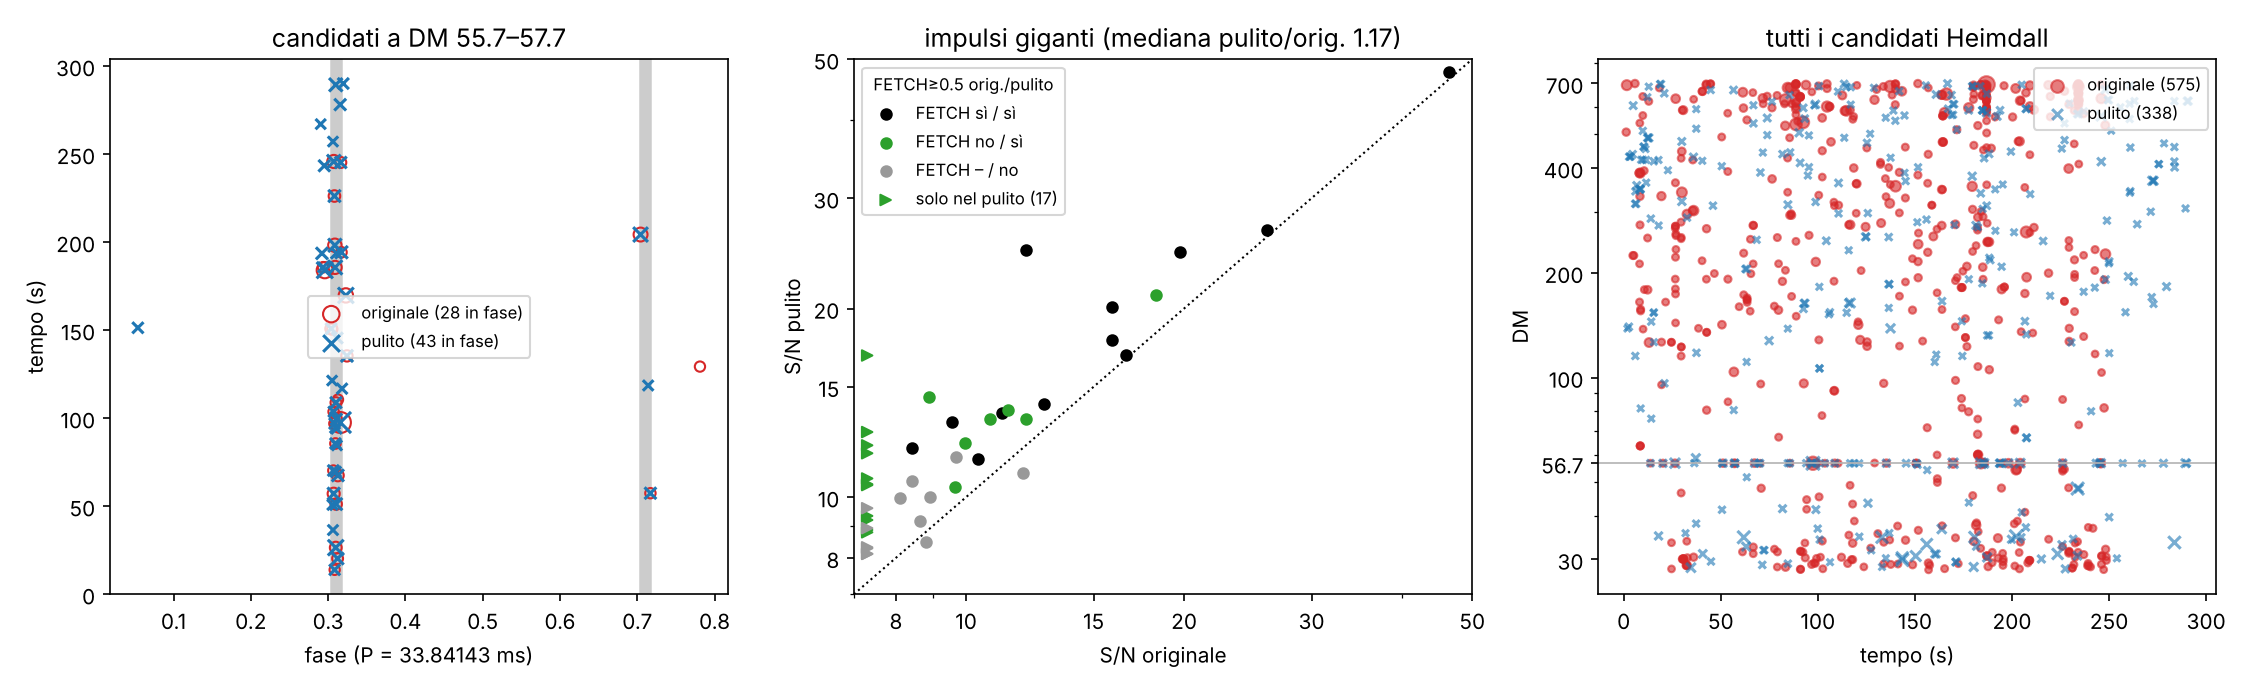
\includegraphics[width=\textwidth]{fig/pipeline/crab_noto_gp.png}
\caption{Crab a Noto, ricerca con \file{FRB_HF_Finder.py} sul file originale (rosso) e pulito (blu). Sinistra: fase
dei candidati a DM 55.7--57.7 per $P=\SI{33.84143}{\milli\second}$ (in grigio le finestre dell'impulso principale e
dell'interimpulso); la dimensione è proporzionale all'S/N. Centro: S/N degli impulsi giganti nel file pulito rispetto
all'originale, con la classificazione FETCH ($\geq0.5$) nei due file; i triangoli a sinistra sono gli impulsi trovati
solo nel file pulito. Destra: tutti i candidati Heimdall nel piano tempo--DM.}
\label{fig:crabnoto}
\end{figure}

\subsection{Un impulso gigante prima e dopo la pulizia}
La Fig.~\ref{fig:crabgp} mostra, con \file{tools/plot_dynspec.py}, \SI{120}{\milli\second} attorno all'impulso gigante
più forte (\SI{97.474}{\second}, S/N 47.6), a DM 0, nel file originale e dopo lo step 4, con la stessa scala di colori.
\begin{itemize}
  \item \textbf{Originale.} La serie a DM 0 è dominata dai lampi della banda \SIrange{1445}{1480}{\mega\hertz} (a circa
    20, 30, 40 e \SI{100}{\milli\second}, alti 2--3 conteggi), che nello spettro dinamico sono blocchi chiari; nella
    stessa banda strisce verticali fitte alternano livelli alti e bassi. Lo spettro medio mostra le portanti a
    \SIrange{1525}{1555}{\mega\hertz} e la depressione del bandpass a \SIrange{1453}{1471}{\mega\hertz}. L'impulso
    gigante è la traccia diagonale debole da circa \SI{55}{\milli\second} (\SI{1606}{\mega\hertz}) a circa
    \SI{92}{\milli\second} (\SI{1350}{\mega\hertz}); nella serie a DM 0 non si vede.
  \item \textbf{Dopo lo step 4.} La serie a DM 0 è piatta, lo spettro medio è piatto, i lampi e le portanti sono
    spariti, il blocco \SIrange{1453}{1471}{\mega\hertz} e i canali a \SI{1381}{\mega\hertz} sono mascherati (rosa).
    La traccia dell'impulso gigante resta intatta ed è ora la struttura più evidente del pannello.
\end{itemize}
È l'illustrazione diretta di quanto misurato con la ricerca: la pulizia rimuove l'RFI a DM 0 e il rumore comune senza
toccare un segnale stretto e disperso.

\begin{figure}[ht]
\centering
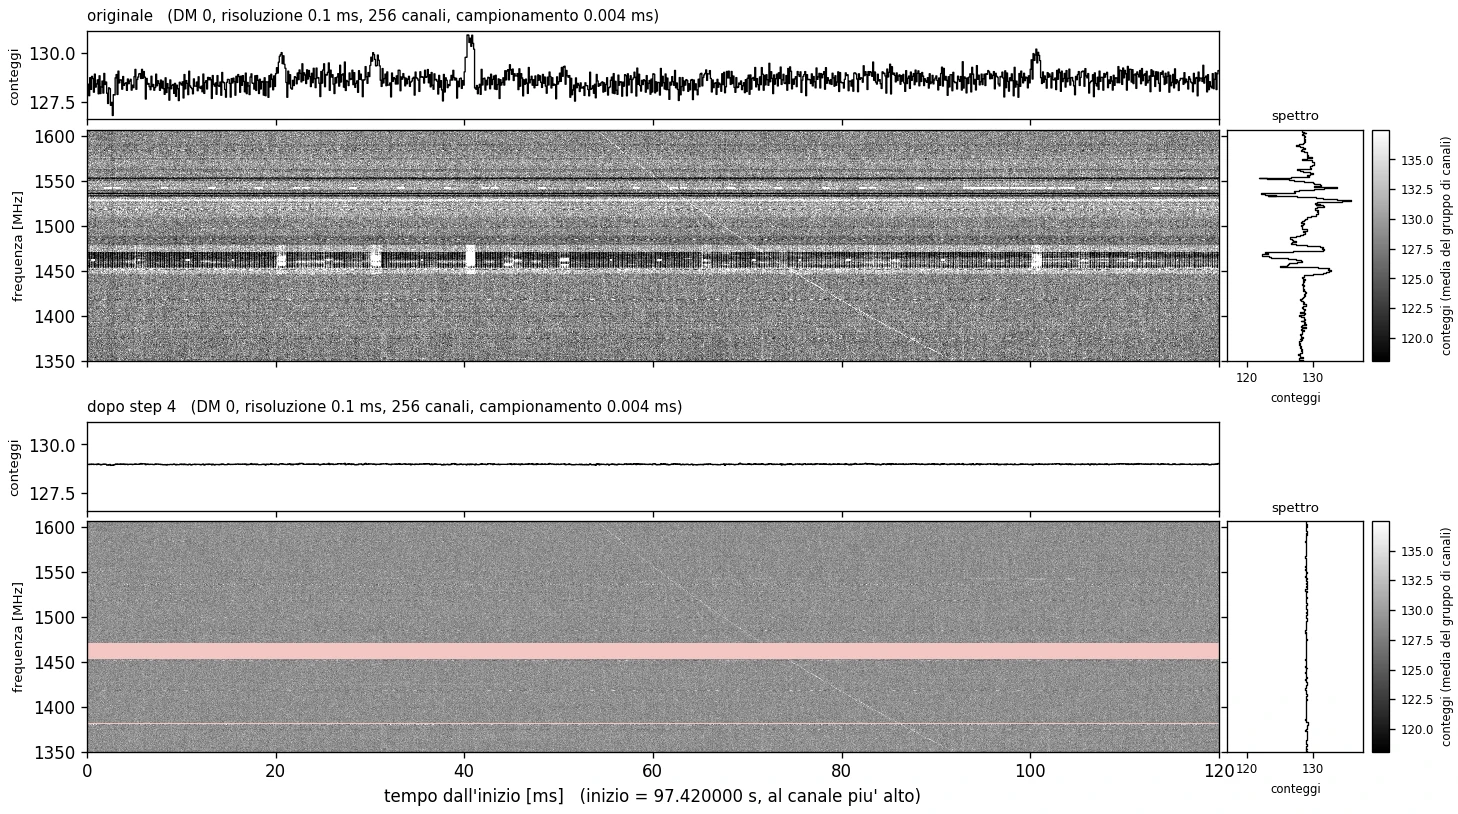
\includegraphics[width=\textwidth]{fig/noto/crab_gp97_dm0.png}
\caption{L'impulso gigante più forte della Crab a Noto (\SI{97.474}{\second}, DM 56.7, S/N 47.6), a DM 0, nel file
originale (sopra) e dopo lo step 4 (sotto): \SI{120}{\milli\second} da \SI{97.42}{\second}, risoluzione
\SI{0.1}{\milli\second}, 256 canali, stessa scala di colori in conteggi. Per ciascun file: serie temporale, spettro
dinamico e spettro medio sulla finestra. Rosa: canali mascherati.}
\label{fig:crabgp}
\end{figure}

\subsection{Ripiegamento e ricerca a singolo impulso con PRESTO}
\sloppy
\begin{itemize}
  \item \textbf{Ripiegamento.} I ripiegamenti con \file{prepfold -psr B0531+21} non mostrano la pulsar in nessuno step.
    Il periodo dato dall'effemeride di TEMPO, \SI{33.84828}{\milli\second}, differisce da quello misurato dagli impulsi
    giganti di \SI{0.0069}{\milli\second} ($2\times10^{-4}$): in \SI{294}{\second} la fase scivola di circa 1.8 giri e
    il profilo si appiattisce. Il parfile usato non è aggiornato: per la Crab, con forte rumore di timing e glitch,
    serve l'effemeride mensile. Il ripiegamento con ricerca in periodo sull'originale ($\chi^2_{\rm red}=47$) e quello a
    parametri fissi ($\chi^2_{\rm red}=15.8$) sono dominati dall'RFI: il primo converge a
    $\dot P=\num{-1.3e-7}$, non fisico, e il secondo scende a $\chi^2_{\rm red}\simeq1.5$ sia con la maschera di
    \file{rfifind} sia dopo lo step 1.
  \item \textbf{Ripiegamento al periodo degli impulsi giganti.} Il periodo ricavato dagli impulsi giganti è
    topocentrico, mentre \file{prepfold -p} lo interpreta come baricentrico se l'header contiene le coordinate: serve
    l'opzione \file{-topo}. Con \file{-topo -nosearch}, $P=\SI{33.841426}{\milli\second}$, DM 56.72 e 128 intervalli,
    la Crab compare negli step 1, 2 e 3: un impulso stretto (un intervallo, \SI{0.26}{\milli\second}) alla stessa fase
    degli impulsi giganti, con un rilievo a DM\,$\simeq$\,56.7 nella curva DM. L'impulso in un solo intervallo
    conferma il periodo entro circa \SI{3e-5}{\milli\second}. La misura dell'S/N del profilo per ogni step è nella
    Tab.~\ref{tab:crabprof} e nella Fig.~\ref{fig:crabprof}.
  \item \textbf{Un picco spurio vicino al periodo della Crab.} Dopo lo step 1 la curva $\chi^2$--periodo di
    \file{prepfold} ha un picco a $P\simeq\SI{33.8459}{\milli\second}$, più alto di quello della pulsar; dopo lo step 2
    scompare e resta solo il picco della Crab. È la famiglia periodica a \SI{12.5}{\hertz} sottratta dallo step 2: la
    sua 26ª armonica (\SI{325}{\hertz}, presente fra le righe trovate) coincide con l'11ª armonica della frequenza di
    ripiegamento, $12.5\times26/11=\SI{29.5454}{\hertz}$, cioè $P=\SI{33.8462}{\milli\second}$. Non è una coincidenza
    fisica: in una finestra di ricerca stretta, attorno a qualunque periodo, qualche armonica di un treno ricco di
    armoniche trova un'armonica del ripiegamento. Senza lo step 2 una ricerca in periodo si sarebbe agganciata all'RFI.
  \item \textbf{S/N del profilo per ogni step} (Tab.~\ref{tab:crabprof}, Fig.~\ref{fig:crabprof}). Stesso metodo di
    B0329+54: segnale integrato sui 3 intervalli dell'impulso principale diviso il rumore robusto fuori impulso. Il
    rumore è confrontato con quello bianco atteso da \file{prepfold} (\emph{Profile StdDev}, dalla deviazione standard
    dei dati) e, per gli step 1--4, con quello radiometrico ($8\sqrt{924}\sqrt{N_{\rm campioni/bin}}$ conteggi).
    \begin{itemize}
      \item Nell'originale il profilo è dominato da variazioni lente dovute all'RFI (rumore 2.3 volte quello bianco):
        S/N 4.4. La maschera di \file{rfifind} e lo step 1 lo portano a 9--10, con rumore vicino a quello bianco.
      \item Gli step 1--3 conservano tutto il segnale (rapporto con lo step 2: 1.01, 1.00, 1.00), e lo step 4 anche
        (0.996), come previsto per un impulso stretto (Sez.~\ref{sec:step4}); è l'opposto di B0329+54 (0.07).
      \item Lo step 4 aumenta però leggermente il rumore del profilo (da 1.29 a 1.45 volte il radiometrico), e l'S/N
        scende da 9.5 a 8.4. La differenza è al limite dell'incertezza della stima del rumore (circa 7\% con circa
        110 intervalli fuori impulso). Qui il rumore del profilo è già vicino al radiometrico dopo lo step 1, quindi lo
        step 4 non ha nulla da guadagnare sul ripiegamento; il suo guadagno è sulla ricerca a singolo impulso.
      \item La maschera di \file{rfifind} dà sul ripiegamento lo stesso risultato della pipeline (9.7 contro 9.5--9.8):
        per il segnale medio di una pulsar la differenza fra i due metodi è trascurabile. La differenza è negli impulsi
        singoli (Tab.~\ref{tab:crabnoto}).
      \item L'interimpulso non è rivelato (meno di 2$\sigma$ in tutti i file).
    \end{itemize}
  \item \textbf{Ricerca a singolo impulso.} Con \file{prepsubband} (DM 30--85, passo 1) e \file{single_pulse_search.py}
    gli eventi passano da 6227 (5260 a DM\,$<$\,50) nell'originale a 111 (27 a DM\,$<$\,50) nel file pulito. Gli
    impulsi giganti sono trovati però con S/N basso (massimo 9.4): con \SI{256}{\mega\hertz} di banda un errore di 0.5
    in DM sbava l'impulso di circa \SI{0.3}{\milli\second}, contro una durata di circa \SI{0.05}{\milli\second}. Per un
    confronto equo serve un passo di circa 0.05 attorno a DM 56.7.
\end{itemize}
\fussy


\begin{table}[ht]
\centering
\caption{Crab a Noto, ripiegamento a $P=\SI{33.841426}{\milli\second}$ (topocentrico), DM 56.72, 128 intervalli: S/N
del profilo (impulso principale, 3 intervalli), rumore fuori impulso rispetto al bianco atteso da \file{prepfold} e al
radiometrico, segnale integrato rispetto allo step 2.}
\label{tab:crabprof}
\small
\begin{tabular}{lccccc}
\toprule
 & S/N del picco & S/N integrato & rumore / bianco & rumore / radiometrico & segnale / step 2 \\
\midrule
originale & 3.7 & 4.4 & 2.26 & -- & -- \\
originale + \file{rfifind} & 8.7 & 9.7 & 1.02 & -- & -- \\
step 1 & 7.8 & 9.1 & 1.14 & 1.37 & 1.01 \\
step 2 & 8.6 & 9.8 & 1.04 & 1.25 & 1.00 \\
step 3 & 8.3 & 9.5 & 1.08 & 1.29 & 1.00 \\
step 4 & 7.4 & 8.4 & 1.21 & 1.45 & 1.00 \\
\bottomrule
\end{tabular}
\end{table}

\begin{figure}[ht]
\centering
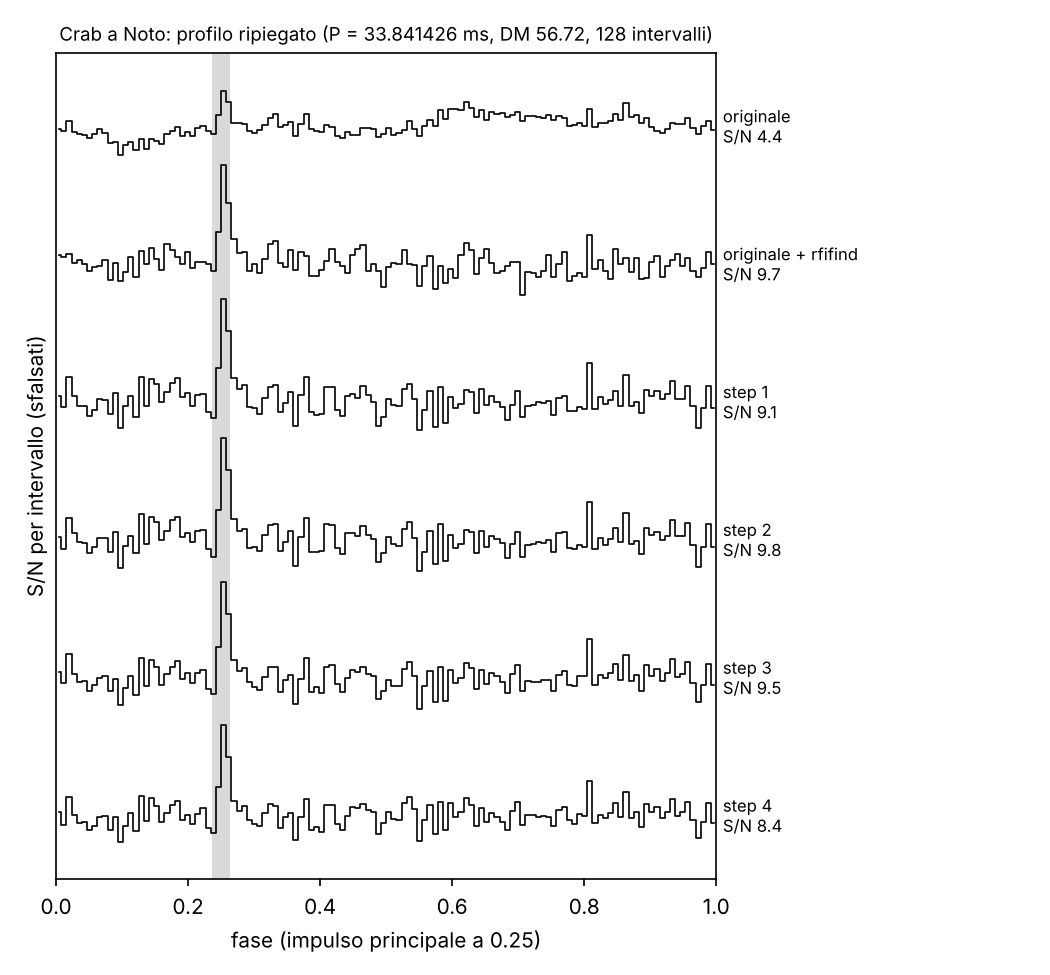
\includegraphics[width=0.75\textwidth]{fig/noto/crab_profiles.png}
\caption{Profili della Crab a Noto (\SI{294}{\second}, 128 intervalli) nel file originale, con la maschera di
\file{rfifind} e dopo ogni step, ciascuno in unità del proprio rumore fuori impulso e sfalsati in verticale. In grigio la
finestra dell'impulso principale usata per l'S/N.}
\label{fig:crabprof}
\end{figure}

% -------------------------------------------------------------------------------------
\subsection{L'ambiente RFI di Noto in banda L}
\label{sec:notoenv}
Il file originale e quello pulito sono stati analizzati con \file{tools/rfi_survey.py} (opzioni di default, con lo
spettro di potenza della serie a DM 0 alla risoluzione nativa, fino a \SI{125}{\kilo\hertz}). È una sola osservazione di
\SI{294}{\second}: il quadro è indicativo, e le identificazioni delle sorgenti sono ipotesi.

\paragraph{Cosa contiene il file originale} (Figg.~\ref{fig:notodyn} e \ref{fig:notospec}).
\begin{itemize}
  \item \textbf{Banda \SIrange{1445}{1495}{\mega\hertz}: la sorgente dominante.} Lampi di qualche secondo, a gruppi,
    per tutta l'osservazione, alternati a fasi in cui il livello scende sotto la mediana. Le stesse fasi producono le
    cadute verso il basso della serie a DM 0 (fino a circa $-8\%$ della potenza totale, a
    \SIrange{130}{160}{\second} e \SIrange{205}{265}{\second}). Nella stessa banda, a \SIrange{1478}{1494}{\mega\hertz},
    c'è un treno di impulsi larghi \SI{0.5}{\milli\second} a \SI{12.5}{\hertz} (4435 eventi, statistica di Rayleigh
    $Z=2408$), la famiglia sottratta dallo step 2. \ipotesi{\SIrange{1452}{1492}{\mega\hertz} è la banda europea della
    telefonia mobile in sola discesa (SDL): un segnale digitale a trame regolari è compatibile. La discesa del livello
    all'arrivo di un segnale forte fa pensare a un controllo automatico del guadagno nel ricevitore o nel backend.}
  \item \textbf{Banda \SIrange{1505}{1575}{\mega\hertz}.} Portanti strette persistenti a \SIrange{1525}{1555}{\mega\hertz},
    con molti valori estremi e livello molto variabile, e una struttura lenta e larga: fra circa 150 e
    \SI{230}{\second} il livello di tutta la banda scende per circa \SI{80}{\second}. \ipotesi{\SIrange{1525}{1559}{\mega\hertz}
    è la banda di discesa dei satelliti per comunicazioni mobili (per esempio Inmarsat).}
  \item \textbf{Portante a \SI{1437}{\mega\hertz}}, stretta e intermittente (\SIrange{8}{70}{\second} e
    \SIrange{190}{250}{\second}).
  \item \textbf{Righe periodiche.} Oltre a \SI{12.5}{\hertz}, righe a 2, 9.5 e \SI{33.3}{\hertz}; nel kHz una famiglia
    a multipli di \SI{2}{\kilo\hertz} (armoniche di \SI{200}{\hertz} fino a \SI{12}{\kilo\hertz}) e righe isolate a 22,
    42, 46, 50, \SI{52}{\kilo\hertz} e oltre, 60 in tutto. \ipotesi{Righe di questo tipo sono tipiche di elettronica
    locale (alimentatori, clock digitali).}
  \item \textbf{Eventi impulsivi a DM 0.} 7623, quasi tutti in una sola sottobanda: 7620 colpiscono al più il 25\% della
    banda, nessuno più del 75\%. S/N massimo 35; 106 eventi con S/N\,$\geq$\,20.
  \item \textbf{Bandpass e guadagno.} Il bandpass è già piatto in ingresso (circa 123 conteggi): il backend equalizza
    la banda, e la sua forma reale non è ricostruibile. 171 salti di guadagno, a intervalli irregolari.
\end{itemize}

\begin{table}[ht]
\centering
\caption{Ambiente RFI in banda L: Medicina (Sez.~\ref{sec:rfienv}) e Noto (questa sezione).}
\label{tab:notoenv}
\small
\begin{tabular}{p{4.2cm}p{4.6cm}p{5.4cm}}
\toprule
 & Medicina & Noto \\
\midrule
radar a banda larga & due, periodo \SI{10}{\second}, dominanti & nessun evento a banda larga \\
rete elettrica & famiglia a \SI{50}{\hertz} & non evidente \\
treni periodici & \SI{1.987}{\hertz} & \SI{12.5}{\hertz}, impulsi da \SI{0.5}{\milli\second} a \SIrange{1478}{1494}{\mega\hertz} \\
righe nel kHz & -- & famiglia a \SI{2}{\kilo\hertz}, righe a \SIrange{22}{52}{\kilo\hertz} \\
RFI in banda & \SIrange{1438}{1440}{\mega\hertz}, \SI{1421}{\mega\hertz} & \SIrange{1445}{1495}{\mega\hertz} (forte),
  \SIrange{1525}{1555}{\mega\hertz}, \SI{1437}{\mega\hertz} \\
eccesso di rumore a DM 0 & 4.4--4.7 & 3.5 (2.5--5.0 fra i blocchi) \\
salti di guadagno & circa ogni \SI{1}{\second} & 171 in \SI{294}{\second}, irregolari \\
\bottomrule
\end{tabular}
\end{table}

\paragraph{Confronto con Medicina} (Tab.~\ref{tab:notoenv}). L'RFI di Noto è soprattutto a banda stretta e
compatibile con servizi di telecomunicazione; a Medicina dominano radar e disturbi locali a banda larga. Il rumore
correlato fra i canali c'è in entrambi i siti, a Noto un po' minore, e anche qui la differenza fra le due metà della
banda (eccesso 2.1) non è descritta da un solo modo comune.

\paragraph{Dopo la pipeline} (Fig.~\ref{fig:notodyn}, sotto). Spariscono il treno a \SI{12.5}{\hertz} (Rayleigh da
1619 a 2.6 su tutti gli eventi), quasi tutte le righe dello spettro (da 60 a 2, al limite della soglia: \SI{2125.85}{\hertz}
e \SI{91.56}{\kilo\hertz}, quest'ultima con periodo di 2.7 campioni, sotto il minimo dello step 2) e gli eventi forti
(S/N\,$\geq$\,20 da 106 a 0, S/N\,$\geq$\,10 da 2000 a 149). Restano:
\begin{itemize}
  \item i \textbf{bordi del blocco mascherato}, \SIrange{1446}{1452}{\mega\hertz} e \SIrange{1472}{1480}{\mega\hertz}: i
    lampi vi sono ancora visibili nel pannello del massimo, e lo step 4 vi trova i guadagni più alti (1.6--1.9 contro
    0.92 in mediana);
  \item impulsi deboli non periodici a \SIrange{1414}{1430}{\mega\hertz} (863 eventi);
  \item le portanti a \SIrange{1525}{1555}{\mega\hertz} e la struttura lenta a \SIrange{1505}{1575}{\mega\hertz}.
\end{itemize}
Sono due limiti dello step 1. (1) Il rumore di ogni canale è confrontato con la mediana dei circa 32 canali vicini: se
un blocco di RFI è largo quanto metà di questa finestra, il riferimento è contaminato e i canali ai bordi sembrano
normali. (2) Ogni canale è riassunto dalla \emph{mediana nel tempo} delle sue statistiche: un RFI presente in meno di
metà dei blocchi non la sposta, per quanto sia forte. I rimedi, che usano statistiche già calcolate, sono un secondo
passaggio della maschera con i riferimenti ricalcolati senza i canali già mascherati e un criterio per l'RFI
intermittente (un percentile alto nel tempo invece della mediana, o la variabilità del livello fra i blocchi). Va
evitato di mascherare la riga dell'idrogeno a \SI{1420.4}{\mega\hertz}, forte in direzione della Crab, che non è RFI.

\begin{figure}[p]
\centering
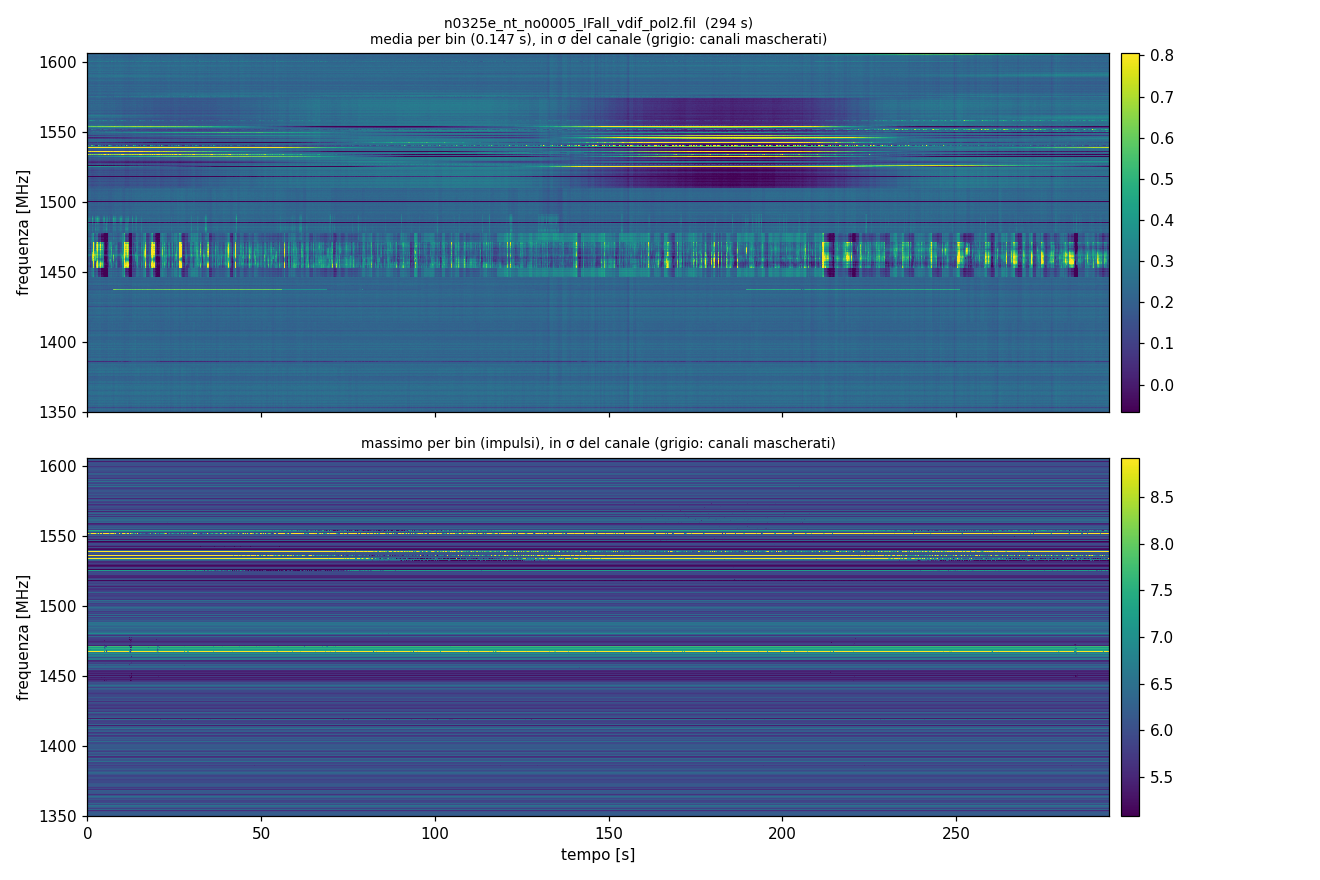
\includegraphics[width=\textwidth]{fig/noto/survey_orig_dynspec.png}\\[2mm]
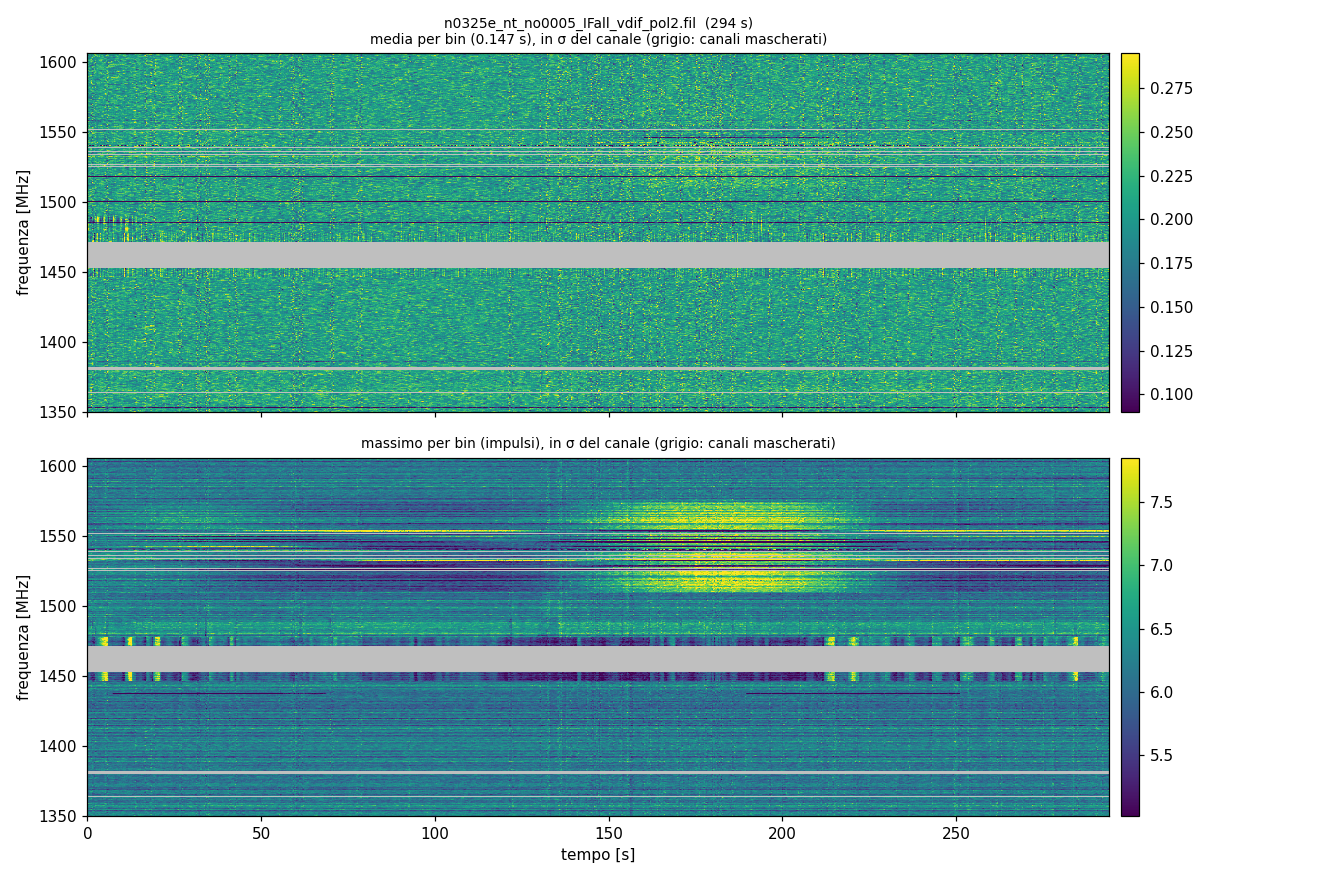
\includegraphics[width=\textwidth]{fig/noto/survey_clean_dynspec.png}
\caption{Censimento di Noto (\file{rfi_survey.py}): spettri dinamici di tutta l'osservazione (\SI{294}{\second},
intervalli di \SI{0.147}{\second}), in unità della $\sigma$ di ciascun canale, nel file originale (sopra) e dopo gli
step 1--4 (sotto). Per ciascuno: media per intervallo (variazioni di livello) e massimo per intervallo (impulsi).
Grigio: canali mascherati.}
\label{fig:notodyn}
\end{figure}

\begin{figure}[ht]
\centering
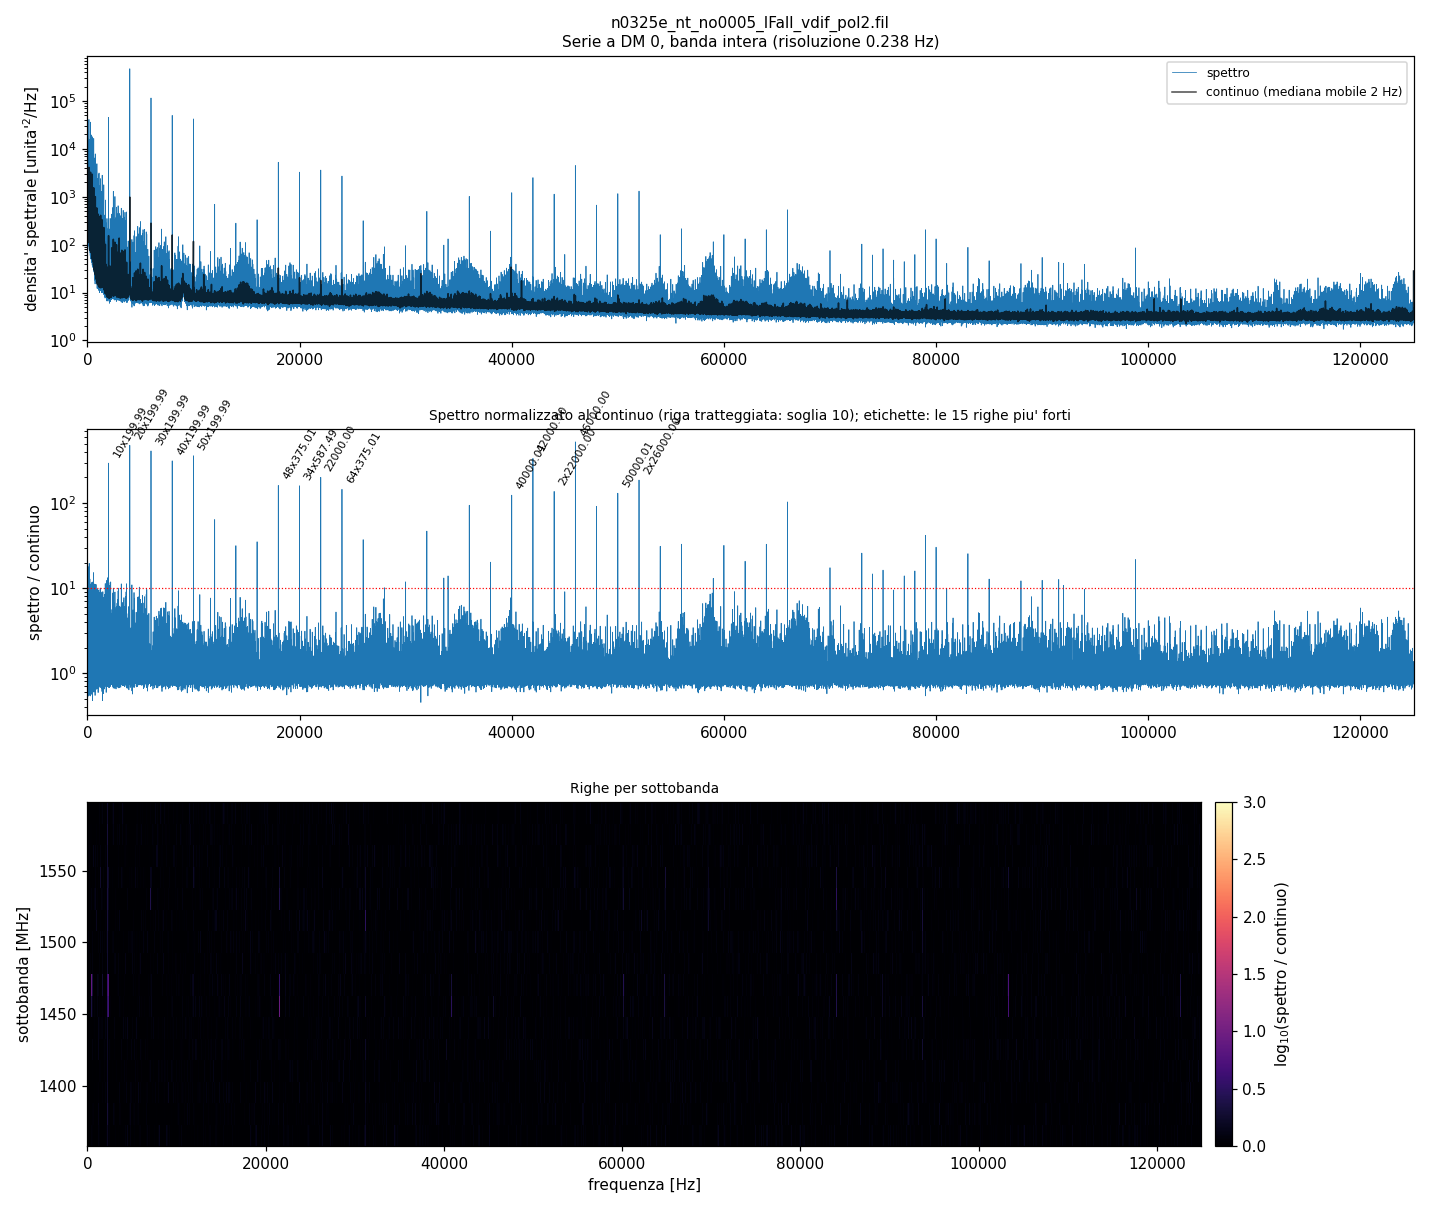
\includegraphics[width=\textwidth]{fig/noto/survey_orig_spectrum.png}
\caption{Spettro di potenza della serie a DM 0 del file originale di Noto (risoluzione \SI{0.24}{\hertz}, fino a
\SI{125}{\kilo\hertz}): spettro e continuo, spettro normalizzato al continuo con le righe più forti, righe per
sottobanda. Dopo la pipeline restano 2 righe al limite della soglia.}
\label{fig:notospec}
\end{figure}


% -------------------------------------------------------------------------------------
\FloatBarrier
\section{Discussione e prossimi passi}
\label{sec:next}

\paragraph{Cosa è stato ottenuto.} Sul file intero la pipeline (step 1--3) riduce i candidati da 2399 a 338, elimina gli
episodi e l'RFI impulsivo a DM 0 forte (eventi a DM 0 con S/N\,$\geq$\,30 da 1105 a 8), riporta l'associazione con i radar
al livello del caso per il radar A e a circa il doppio per il radar B, e azzera i falsi FETCH. Il pilota mostra che la
pulizia aumenta anche la \emph{sensibilità}: i burst rivelati passano da 28 a 73 su 133 con gli step 1--3 e a 103 con lo
step 4. I candidati che restano dopo lo step 3 sono una popolazione diversa: per il 42\% larghi $\geq\SI{4}{\milli\second}$,
con DM mediano 167, e solo per il 37\% associati a un evento a DM 0 nel proprio sweep (per caso il 6\%). Sono emissioni a
banda stretta più lunghe di \SI{32}{\milli\second} e variazioni lente, che lo step 3 non è progettato per trattare.
Su un'osservazione indipendente (la Crab a Noto, Sez.~\ref{sec:crabnoto}), con un'altra antenna e un altro setup e con i
valori di default, la pipeline completa (step 1--4) porta gli impulsi giganti rivelati da 28 a 43 (accettati da FETCH da
13 a 30), ne migliora l'S/N in mediana del 17\% e dimezza i falsi candidati.

\paragraph{Limiti.}
\begin{itemize}
  \item Sviluppo su una sola osservazione. Il test sulla Crab a Noto (1024 canali, \SI{4}{\micro\second},
    \SI{256}{\mega\hertz}) mostra che i default funzionano anche su un altro setup; resta da provare un dataset a banda
    stretta e frequenza bassa, come quelli della Croce del Nord.
  \item Il numero di sottobande (16) è fisso: su bande strette andrebbe legato alla larghezza di banda o al numero di canali.
  \item Lo step 3 protegge 1221 eventi deboli (S/N mediano 7.5 a DM 0); il veto non è ancora tarato su dati reali.
  \item Il pilota ha 7 burst per punto e un solo file; lo step 4 vi è nella prima versione.
  \item Il test su B0329+54 (Sez.~\ref{sec:b0329}) conferma su dati reali il limite larghezza/sweep: per una pulsar
    con impulsi più larghi del proprio sweep lo step 3 conserva il 92\% del segnale e lo step 4 solo il 7\%. Con lo step 4
    attivo, i burst larghi qualche millisecondo a DM sotto circa 50--100 vengono persi.
  \item Canali con RFI persistente a banda stretta (\SIrange{1438}{1440}{\mega\hertz}, \SI{1421}{\mega\hertz}) non sono
    mascherati: i tratti sostituiti li rendono più gaussiani degli altri canali, ma lasciano una piccola variabilità.
\end{itemize}

\paragraph{Prossimi passi.}
\begin{enumerate}
  \item Ripetere il pilota con la versione attuale dello step 4 e verificare che i falsi candidati larghi tornino al
    livello dello step 3.
  \item Ricerca sul file intero dopo lo step 4 (confronto con i 338 candidati dello step 3).
  \item Campagna di completezza completa: 4 realizzazioni del file intero, scansioni A--E, circa 2000 burst, con la
    calibrazione dell'S/N ricavata dal file di solo rumore.
  \item Se i falsi larghi restano: guadagni dello step 4 interpolati tra i blocchi e sottrazione di più componenti correlate
    (2--3), misurandone il costo per gli FRB.
  \item Valutare un trattamento delle emissioni a banda stretta più lunghe di \SI{32}{\milli\second}.
  \item Sostituzione dei default legati alla geometria con valori derivati
    dall'header.
  \item Per lo step 4: renderlo facoltativo, oppure eseguire la ricerca sia dopo lo step 3 sia dopo lo step 4 e unire i
    candidati, oppure non sottrarre il modo comune dove contiene un segnale disperso; il ripiegamento di B0329+54 è il
    test per valutarlo.
  \item Step 1: secondo passaggio della maschera (bordi dei blocchi larghi) e criterio per l'RFI intermittente, come
    indicato dal censimento di Noto (Sez.~\ref{sec:notoenv}), senza mascherare la riga dell'HI.
  \item Efficienza di FETCH in funzione dell'S/N: sulla Crab FETCH scarta gli impulsi veri sotto S/N circa 11--12; la
    campagna di completezza la misura direttamente (rivelati con FETCH\,$\geq$\,0.5 e 0.7).
  \item Velocità: \SI{4.7}{\hour} per un file di \SI{75}{\giga\byte}; per un uso sistematico serve parallelizzare.
  \item Integrazione in \file{FRB_HF_Finder.py}, come per il ramo IQRM.
\end{enumerate}


% =====================================================================================
\appendix
\FloatBarrier
\section{Riproducibilità}
\label{app:repro}

\begin{itemize}
  \item Codice: \url{https://github.com/davidepelliciari/frb-rfi-clean}. Strumenti in \file{tools/},
    \file{injection/}, \file{frbclean/}; test in \file{tests/}.
  \item Censimento sul file completo, eseguito sul cluster di Medicina con i parametri di default:
\begin{Verbatim}[fontsize=\small,breaklines=true]
python3 tools/rfi_survey.py ag278m_mc_no0004_processed.fil --out survey_no0004_full/
\end{Verbatim}
    I parametri sono riportati nella Tab.~\ref{tab:surveycfg}. Il file \file{survey.npz} è nel repository \url{https://github.com/davidepelliciari/frb-rfi-data},\\
    cartella \file{surveys/ag278m_mc_no0004_full/}.
  \item \file{docs/report_no0004/data/} contiene i prodotti tabulari del censimento e i CSV della pipeline di
    ricerca.
  \item Figure, tabelle e numeri di questo documento:
\begin{Verbatim}[fontsize=\small,breaklines=true]
python3 docs/report_no0004/analysis.py --npz <percorso>/survey.npz
\end{Verbatim}
    Lo script scrive \file{fig/}, \file{tab_*.tex} e \file{numbers.json}.
  \item Pipeline di pulizia, nell'ordine (ogni step scrive accanto all'output un riassunto \file{.json}):
\begin{Verbatim}[fontsize=\small,breaklines=true]
python3 tools/rfi_clean.py      originale.fil step1.fil
python3 tools/rfi_periodic.py   step1.fil     step2.fil
python3 tools/rfi_impulses.py   step2.fil     step3.fil
python3 tools/rfi_commonmode.py step3.fil     step4.fil
\end{Verbatim}
    I risultati delle ricerche e dei censimenti dopo ogni step sono in \url{https://github.com/davidepelliciari/frb-rfi-data},
    cartelle \file{search/} e \file{surveys/} (\file{..._clean_step1}, \file{..._step2_updated},
    \file{..._step3_v4}, \file{..._step4}).
  \item Campagna di completezza (piano, una realizzazione, associazione e resoconto):
\begin{Verbatim}[fontsize=\small,breaklines=true]
python3 injection/completeness_plan.py --fil originale.fil --outdir camp --seed 1
bash injection/run_realization.sh originale.fil camp/real_01.params lavoro_r01 1
python3 injection/recover.py match --plan camp/plan.csv --realization 1 --step orig lavoro_r01/orig ... --out camp/matched_r01.csv
python3 injection/recover.py report --matched 'camp/matched_r*.csv' --out camp/report
\end{Verbatim}
    I prodotti del pilota sono in \file{completeness/pilot/} del repository dei dati.
  \item Figure della pipeline: \file{fig/pipeline/} (la Fig.~\ref{fig:final} è prodotta con
    \file{tools/plot_dynspec.py}).
  \item Validazione di tutti gli strumenti: \texttt{python3 -m pytest tests} (47 test).
\end{itemize}

\begin{table}[ht]
\centering
\caption{Parametri del censimento usati per il file completo.}
\label{tab:surveycfg}
\begin{tabular}{ll}
\toprule
Sottobande & 16 (\SI{4}{\mega\hertz}) \\
Larghezze dei boxcar & $2^k\,t_{\rm samp}$, $k=0..11$ (\SIrange{0.016}{32.8}{\milli\second}) \\
Soglia eventi / soglia sottobanda colpita & S/N 6 / S/N 3 \\
Durata dei blocchi & \SI{4.19}{\second} \\
Finestra della baseline per gli eventi & \SI{0.26}{\second} \\
Spettro dinamico ridotto & 2000 bin (\SI{0.6}{\second}) \\
Serie a DM 0 salvata & \SI{1.024}{\milli\second} \\
Soglia z per i canali & 5 \\
\bottomrule
\end{tabular}
\end{table}

\end{document}
